% 若编译失败,且生成 .synctex(busy) 辅助文件,可能有两个原因:
% 1. 需要插入的图片不存在:Ctrl + F 搜索 'figure' 将这些代码注释/删除掉即可
% 2. 路径/文件名含中文或空格:更改路径/文件名即可

% --------------------- 文章宏包及相关设置 --------------------- %
% >> ------------------ 文章宏包及相关设置 ------------------ << %
% 设定文章类型与编码格式
\documentclass[UTF8]{article}		

% 物理实验报告所需的其它宏包
\usepackage{ulem}   % \uline 下划线支持
\usepackage{circuitikz} % 电路图 tikz 支持
\usepackage{pdfpages}   % 用于导入 pdf 文件

% 本 .tex 专属的宏定义
    \def\V{\ \mathrm{V}}
    \def\uV{\ \mu\mathrm{V}}
    \def\mV{\ \mathrm{mV}}
    \def\K{\ \mathrm{K}}
    \def\kV{\ \mathrm{KV}}
    \def\KV{\ \mathrm{KV}}
    \def\MV{\ \mathrm{MV}}
    \def\uA{\ \mu\mathrm{A}}
    \def\mA{\ \mathrm{mA}}
    \def\A{\ \mathrm{A}}
    \def\kA{\ \mathrm{KA}}
    \def\KA{\ \mathrm{KA}}
    \def\MA{\ \mathrm{MA}}
    \def\O{\ \Omega}
    \def\mO{\ \Omega}
    \def\kO{\ \mathrm{K}\Omega}
    \def\KO{\ \mathrm{K}\Omega}
    \def\MO{\ \mathrm{M}\Omega}
    \def\Hz{\ \mathrm{Hz}}
    \def\uF{\ \mu\mathrm{F}}
    \def\mF{\ \mathrm{mF}}
    \def\F{\ \mathrm{F}}

% 自定义宏定义
    \def\N{\mathbb{N}}
    \def\F{\mathbb{F}}
    \def\Z{\mathbb{Z}}
    \def\Q{\mathbb{Q}}
    \def\R{\mathbb{R}}
    \def\C{\mathbb{C}}
    \def\T{\mathbb{T}}
    \def\S{\mathbb{S}}
    %\def\A{\mathbb{A}}
    \def\I{\mathscr{I}}
    \def\d{\mathrm{d}}
    \def\p{\partial}


% 导入基本宏包
    \usepackage[UTF8]{ctex}     % 设置文档为中文语言
    \usepackage{hyperref}  % 宏包:自动生成超链接 (此宏包与标题中的数学环境冲突)
    \hypersetup{
        colorlinks=true,    % false:边框链接 ; true:彩色链接
        citecolor={blue},    % 文献引用颜色
        linkcolor={blue},   % 目录 (我们在目录处单独设置),公式,图表,脚注等内部链接颜色
        urlcolor={orange},    % 网页 URL 链接颜色,包括 \href 中的 text
        % cyan 浅蓝色 
        % magenta 洋红色
        % yellow 黄色
        % black 黑色
        % white 白色
        % red 红色
        % green 绿色
        % blue 蓝色
        % gray 灰色
        % darkgray 深灰色
        % lightgray 浅灰色
        % brown 棕色
        % lime 石灰色
        % olive 橄榄色
        % orange 橙色
        % pink 粉红色
        % purple 紫色
        % teal 蓝绿色
        % violet 紫罗兰色
    }
    % \usepackage{docmute}    % 宏包:子文件导入时自动去除导言区,用于主/子文件的写作方式,\include{./51单片机笔记}即可。注:启用此宏包会导致.tex文件capacity受限。
    \usepackage{amsmath}    % 宏包:数学公式
    \usepackage{mathrsfs}   % 宏包:提供更多数学符号
    \usepackage{amssymb}    % 宏包:提供更多数学符号
    \usepackage{pifont}     % 宏包:提供了特殊符号和字体
    \usepackage{extarrows}  % 宏包:更多箭头符号 
    \usepackage{multicol}   % 宏包:支持多栏 

% 文章页面margin设置
    \usepackage[a4paper]{geometry}
        \geometry{top=0.75in}
        \geometry{bottom=0.75in}
        \geometry{left=0.75in}
        \geometry{right=0.75in}   % 设置上下左右页边距
        \geometry{marginparwidth=1.75cm}    % 设置边注距离(注释、标记等)

% 配置数学环境
    \usepackage{amsthm} % 宏包:数学环境配置
    % theorem-line 环境自定义
        \newtheoremstyle{MyLineTheoremStyle}% <name>
            {11pt}% <space above>
            {11pt}% <space below>
            {\kaishu}% <body font> 默认使用正文字体, \kaishu 为楷体
            {}% <indent amount>
            {\bfseries}% <theorem head font> 设置标题项为加粗
            {:\ \ }% <punctuation after theorem head>
            {.5em}% <space after theorem head>
            {\textbf{#1}\thmnumber{#2}\ \ (\,\textbf{#3}\,)}% 设置标题内容顺序
        \theoremstyle{MyLineTheoremStyle} % 应用自定义的定理样式
        \newtheorem{LineTheorem}{Theorem.\,}
    % theorem-block 环境自定义
        \newtheoremstyle{MyBlockTheoremStyle}% <name>
            {11pt}% <space above>
            {11pt}% <space below>
            {\kaishu}% <body font> 使用默认正文字体
            {}% <indent amount>
            {\bfseries}% <theorem head font> 设置标题项为加粗
            {:\\ \indent}% <punctuation after theorem head>
            {.5em}% <space after theorem head>
            {\textbf{#1}\thmnumber{#2}\ \ (\,\textbf{#3}\,)}% 设置标题内容顺序
        \theoremstyle{MyBlockTheoremStyle} % 应用自定义的定理样式
        \newtheorem{BlockTheorem}[LineTheorem]{Theorem.\,} % 使用 LineTheorem 的计数器
    % definition 环境自定义
        \newtheoremstyle{MySubsubsectionStyle}% <name>
            {11pt}% <space above>
            {11pt}% <space below>
            {}% <body font> 使用默认正文字体
            {}% <indent amount>
            {\bfseries}% <theorem head font> 设置标题项为加粗
            {:\\ \indent}% <punctuation after theorem head>
            {0pt}% <space after theorem head>
            {\textbf{#3}}% 设置标题内容顺序
        \theoremstyle{MySubsubsectionStyle} % 应用自定义的定理样式
        \newtheorem{definition}{}

%宏包:有色文本框(proof环境)及其设置
    \usepackage{xcolor}    %设置插入的文本框颜色
    \usepackage[strict]{changepage}     % 提供一个 adjustwidth 环境
    \usepackage{framed}     % 实现方框效果
        \definecolor{graybox_color}{rgb}{0.95,0.95,0.96} % 文本框颜色。修改此行中的 rgb 数值即可改变方框纹颜色,具体颜色的rgb数值可以在网站https://colordrop.io/ 中获得。(截止目前的尝试还没有成功过,感觉单位不一样)(找到喜欢的颜色,点击下方的小眼睛,找到rgb值,复制修改即可)
        \newenvironment{graybox}{%
        \def\FrameCommand{%
        \hspace{1pt}%
        {\color{gray}\vrule width 2pt}%
        {\color{graybox_color}\vrule width 4pt}%
        \colorbox{graybox_color}%
        }%
        \MakeFramed{\advance\hsize-\width\FrameRestore}%
        \noindent\hspace{-4.55pt}% disable indenting first paragraph
        \begin{adjustwidth}{}{7pt}%
        \vspace{2pt}\vspace{2pt}%
        }
        {%
        \vspace{2pt}\end{adjustwidth}\endMakeFramed%
        }

% 外源代码插入设置
    % matlab 代码插入设置
    \usepackage{matlab-prettifier}
        \lstset{style=Matlab-editor}    % 继承 matlab 代码高亮 , 此行不能删去
    \usepackage[most]{tcolorbox} % 引入tcolorbox包 
    \usepackage{listings} % 引入listings包
        \tcbuselibrary{listings, skins, breakable}
        \newfontfamily\codefont{Consolas} % 定义需要的 codefont 字体
        \lstdefinestyle{MatlabStyle_inc}{   % 插入代码的样式
            language=Matlab,
            basicstyle=\footnotesize\ttfamily\codefont,    % ttfamily 确保等宽 
            breakatwhitespace=false,
            breaklines=true,
            captionpos=b,
            keepspaces=true,
            numbers=left,
            numbersep=15pt,
            showspaces=false,
            showstringspaces=false,
            showtabs=false,
            tabsize=2,
            xleftmargin=15pt,   % 左边距
            %frame=single, % single 为包围式单线框
            frame=shadowbox,    % shadowbox 为带阴影包围式单线框效果
            %escapeinside=``,   % 允许在代码块中使用 LaTeX 命令 (此行无用)
            %frameround=tttt,    % tttt 表示四个角都是圆角
            framextopmargin=0pt,    % 边框上边距
            framexbottommargin=0pt, % 边框下边距
            framexleftmargin=5pt,   % 边框左边距
            framexrightmargin=5pt,  % 边框右边距
            rulesepcolor=\color{red!20!green!20!blue!20}, % 阴影框颜色设置
            %backgroundcolor=\color{blue!10}, % 背景颜色
        }
        \lstdefinestyle{MatlabStyle_src}{   % 插入代码的样式
            language=Matlab,
            basicstyle=\small\ttfamily\codefont,    % ttfamily 确保等宽 
            breakatwhitespace=false,
            breaklines=true,
            captionpos=b,
            keepspaces=true,
            numbers=left,
            numbersep=15pt,
            showspaces=false,
            showstringspaces=false,
            showtabs=false,
            tabsize=2,
        }
        \newtcblisting{matlablisting}{
            %arc=2pt,        % 圆角半径
            % 调整代码在 listing 中的位置以和引入文件时的格式相同
            top=0pt,
            bottom=0pt,
            left=-5pt,
            right=-5pt,
            listing only,   % 此句不能删去
            listing style=MatlabStyle_src,
            breakable,
            colback=white,   % 选一个合适的颜色
            colframe=black!0,   % 感叹号后跟不透明度 (为 0 时完全透明)
        }
        \lstset{
            style=MatlabStyle_inc,
        }

% table 支持
    \usepackage{booktabs}   % 宏包:三线表
    \usepackage{tabularray} % 宏包:表格排版
    \usepackage{longtable}  % 宏包:长表格

% figure 设置
    \usepackage{graphicx}  % 支持 jpg, png, eps, pdf 图片 
    \usepackage{svg}       % 支持 svg 图片
        \svgsetup{
            % 指向 inkscape.exe 的路径
            inkscapeexe = C:/aa_MySame/inkscape/bin/inkscape.exe, 
            % 一定程度上修复导入后图片文字溢出几何图形的问题
            inkscapelatex = false                 
        }
    \usepackage{subcaption} % 用于子图和小图注  

% 图表进阶设置
    \usepackage{caption}    % 图注、表注
        \captionsetup[figure]{name=图}  
        \captionsetup[table]{name=表}
        \captionsetup{
            labelfont=bf, % 设置标签为粗体
            textfont=bf,  % 设置文本为粗体
            font=small  
        }
    \usepackage{float}     % 图表位置浮动设置 
    \usepackage{etoolbox} % 用于保证图注表注的数学字符为粗体
        \AtBeginEnvironment{figure}{\boldmath} % 图注中的数学字符为粗体
        \AtBeginEnvironment{table}{\boldmath}  % 表注中的数学字符为粗体
        \AtBeginEnvironment{tabular}{\unboldmath}   % 保证表格中的数学字符不受额外影响

% 圆圈序号自定义
    \newcommand*\circled[1]{\tikz[baseline=(char.base)]{\node[shape=circle,draw,inner sep=0.8pt, line width = 0.03em] (char) {\bfseries #1};}}   % TikZ solution

% 列表设置
    \usepackage{enumitem}   % 宏包:列表环境设置
        \setlist[enumerate]{
            label=(\arabic*) ,   % 设置序号样式为加粗的 (1) (2) (3)
            ref=\arabic*, % 如果需要引用列表项,这将决定引用格式(这里仍然使用数字)
            itemsep=0pt, parsep=0pt, topsep=0pt, partopsep=0pt, leftmargin=3.5em} 
        \setlist[itemize]{itemsep=0pt, parsep=0pt, topsep=0pt, partopsep=0pt, leftmargin=3.5em}
        \newlist{circledenum}{enumerate}{1} % 创建一个新的枚举环境  
        \setlist[circledenum,1]{  
            label=\protect\circled{\arabic*}, % 使用 \arabic* 来获取当前枚举计数器的值,并用 \circled 包装它  
            ref=\arabic*, % 如果需要引用列表项,这将决定引用格式(这里仍然使用数字)
            itemsep=0pt, parsep=0pt, topsep=0pt, partopsep=0pt, leftmargin=3.5em
        }  

% 其它设置
    % 脚注设置
        \renewcommand\thefootnote{\ding{\numexpr171+\value{footnote}}}
    % 参考文献引用设置
        \bibliographystyle{unsrt}   % 设置参考文献引用格式为unsrt
        \newcommand{\upcite}[1]{\textsuperscript{\cite{#1}}}     % 自定义上角标式引用
    % 文章序言设置
        \newcommand{\cnabstractname}{序言}
        \newenvironment{cnabstract}{%
            \par\Large
            \noindent\mbox{}\hfill{\bfseries \cnabstractname}\hfill\mbox{}\par
            \vskip 2.5ex
            }{\par\vskip 2.5ex}

% 文章默认字体设置
    \usepackage{fontspec}   % 宏包:字体设置
        \setmainfont{SimSun}    % 设置中文字体为宋体字体
        \setCJKmainfont[AutoFakeBold=3]{SimSun} % 设置加粗字体为 SimSun 族,AutoFakeBold 可以调整字体粗细
        \setmainfont{Times New Roman} % 设置英文字体为Times New Roman

% 各级标题自定义设置
    \usepackage{titlesec}   
        % section标题自定义设置 
        \titleformat{\section}[hang]{\normalfont\Large\bfseries\boldmath}{\thesection}{8pt}{}
        % subsection 标题自定义设置
        \titleformat{\subsection}[hang]{\normalfont\large\bfseries\boldmath}{\thesubsection}{8pt}{}
        \titlespacing*{\subsection}{0pt}{6pt}{3pt} % 控制上下间距


% --------------------- 文章宏包及相关设置 --------------------- %
% >> ------------------ 文章宏包及相关设置 ------------------ << %


% ------------------------ 文章信息区 ------------------------ %
% ------------------------ 文章信息区 ------------------------ %
% 页眉页脚设置
\usepackage{fancyhdr}   %宏包:页眉页脚设置
    \pagestyle{fancy}
    \fancyhf{}
    \cfoot{\thepage}
    \renewcommand\headrulewidth{1pt}
    \renewcommand\footrulewidth{0pt}
    \rhead{\bfseries \large {\color{red} 分组序号: 2-05}}    
    \chead{《基础物理实验》实验报告,\ 丁毅,\ 2023K8009908031}
    \lhead{Ex.8 磁滞回线 (2024.10.22)}

% 文档信息设置
%\title{这里是标题\\The Title of the Report}
%\author{丁毅\\ \footnotesize 中国科学院大学,北京 100049\\ Yi Ding \\ %\footnotesize University of Chinese Academy of Sciences, Beijing %100049, China}
%\date{\footnotesize 2024.8 -- 2025.1}

% 开始编辑文章

\begin{document}
%\noindent\begin{flushright}
%    \zihao{2}{分组序号: YK02-2}
%\end{flushright}

%\setCJKfamilyfont{boldsong}[AutoFakeBold = {2.17}]{SimSun}
%\newcommand*{\boldsong}{\CJKfamily{boldsong}}

\begin{center}\large
    \vspace*{-0.8cm}
    \noindent{\huge\bfseries《\ \ 基\ \ 础\ \ 物\ \ 理\ \ 实\ \ 验\ \ \ 》\ \ 实\ \ 验\ \ 报\ \ 告 }
    \\\vspace{0.1cm}
    \noindent{
    {\bfseries 
    实验名称:\uline{\hspace{1.25cm} 观测铁磁材料的磁滞回线 \hspace{1.25cm}}
    }\hspace{0.4cm}
    指导教师:\uline{\hspace{0.3cm}朱中柱\ \ zhuzz@ihep.ac.cn\hspace{0.3cm}}
    }
    \\\vspace{0.1cm}
    \noindent
    {
    姓名:\uline{\,\,\,丁毅\,\,\,}\hspace{0.2cm}
    学号:\uline{\,\,\,{ 2023K8009908031}\,\,\,}\hspace{0.2cm}
    班级/专业:\uline{\,\,\,{2308/电子信息}\,\,\,}\hspace{0.2cm}
    分组序号:\uline{\,\,\,{2-05}\,\,\,}
    }
    \\\vspace{0.1cm}
    \noindent{
    实验日期:\uline{\,\,{ 2024.10.22}\,\,}\hspace{0.2cm}
    实验地点:\uline{\,\,\,教学楼{ 713}\,\,\,}\hspace{0.2cm}
    是否调课/补课:\uline{\hspace{0.26cm}否 \hspace{0.26cm}}\hspace{0.2cm}
    成绩:\uline{\hspace{2cm}}
    }
\end{center}
\vspace{-0.4cm}
\noindent\rule{\textwidth}{0.075em}   % 分割线
\vspace{-1.0cm}
% ------------------------ 文章信息区 ------------------------ %
% ------------------------ 文章信息区 ------------------------ %


% 目录
\setcounter{tocdepth}{3}  % 目录深度为 2(不显示 subsubsection)
\noindent\tableofcontents\thispagestyle{fancy}   % 显示页码、页眉等

% 控制目录不换页
%\vspace{1cm}
%\setcounter{tocdepth}{2}  % 目录深度为 2(不显示 subsubsection)
%\noindent\begin{minipage}{\textwidth}
%\tableofcontents\thispagestyle{fancy}   % 显示页码、页眉等   
%\end{minipage}  

\newpage
\rhead{\bfseries 分组序号: 2-05}



% >> --------------------- 下面是正文内容 --------------------- << %
% ------------------------ 下面是正文内容 ------------------------ %
% ------------------------ 下面是正文内容 ------------------------ %
% ------------------------ 下面是正文内容 ------------------------ %
% ------------------------ 下面是正文内容 ------------------------ %
% >> --------------------- 下面是正文内容 --------------------- << %



\section{实验目的}

\begin{enumerate}
\item 掌握利用示波器测量铁磁材料动态磁滞回线的方法;
\item 掌握利用霍尔传感器测量铁磁材料(准)静态磁滞回线的方法;
\item 了解铁磁性材料的磁化特性;
\item 了解磁滞、磁滞回线和磁化曲线的概念,加深对饱和磁化强度、剩余磁化强度、矫顽力等物理量的理解。
\end{enumerate}


\section{实验仪器}

\subsection{DH4516 磁特性综合测量实验仪等}

DH4516 磁特性综合测量实验仪(包括正弦波信号源,待测样品及绕组,积分电路所用的电阻和电容)、双通道示波器、直流电源、电感、数字多用表。

其中,磁特性综合测量实验仪的主要技术参数如下表所示:

\begin{table}[H]\centering
    %\renewcommand{\arraystretch}{1.5} % 调整行间距为 1.5 倍
    %\setlength{\tabcolsep}{1.5mm} % 调整列间距
    \caption{磁特性综合测量实验仪主要技术参数}
    \label{磁特性综合测量实验仪主要技术参数}
\begin{tabular}{cccccccccc}\toprule
    样品 & 磁滞损耗 & 平均磁路长度 $l$ & 截面面积 $S$ & 线圈匝数 $N$  \\
    \midrule
    样品 1(锰锌铁氧体)  & 较小 &  0.130 m & 1.24 $\times 10^{-4}\  \mathrm{m^2}$ & $N_1 = N_2 = N_3 = 150$\\
    样品 2(EI 型硅钢片) & 较大 &  0.075 m & 1.20 $\times 10^{-4}\  \mathrm{m^2}$ & $N_1 = N_2 = N_3 = 150$\\
    \bottomrule
\end{tabular}
\end{table}

\begin{figure}[H]\centering
\begin{subfigure}[b]{0.5\columnwidth}\centering
    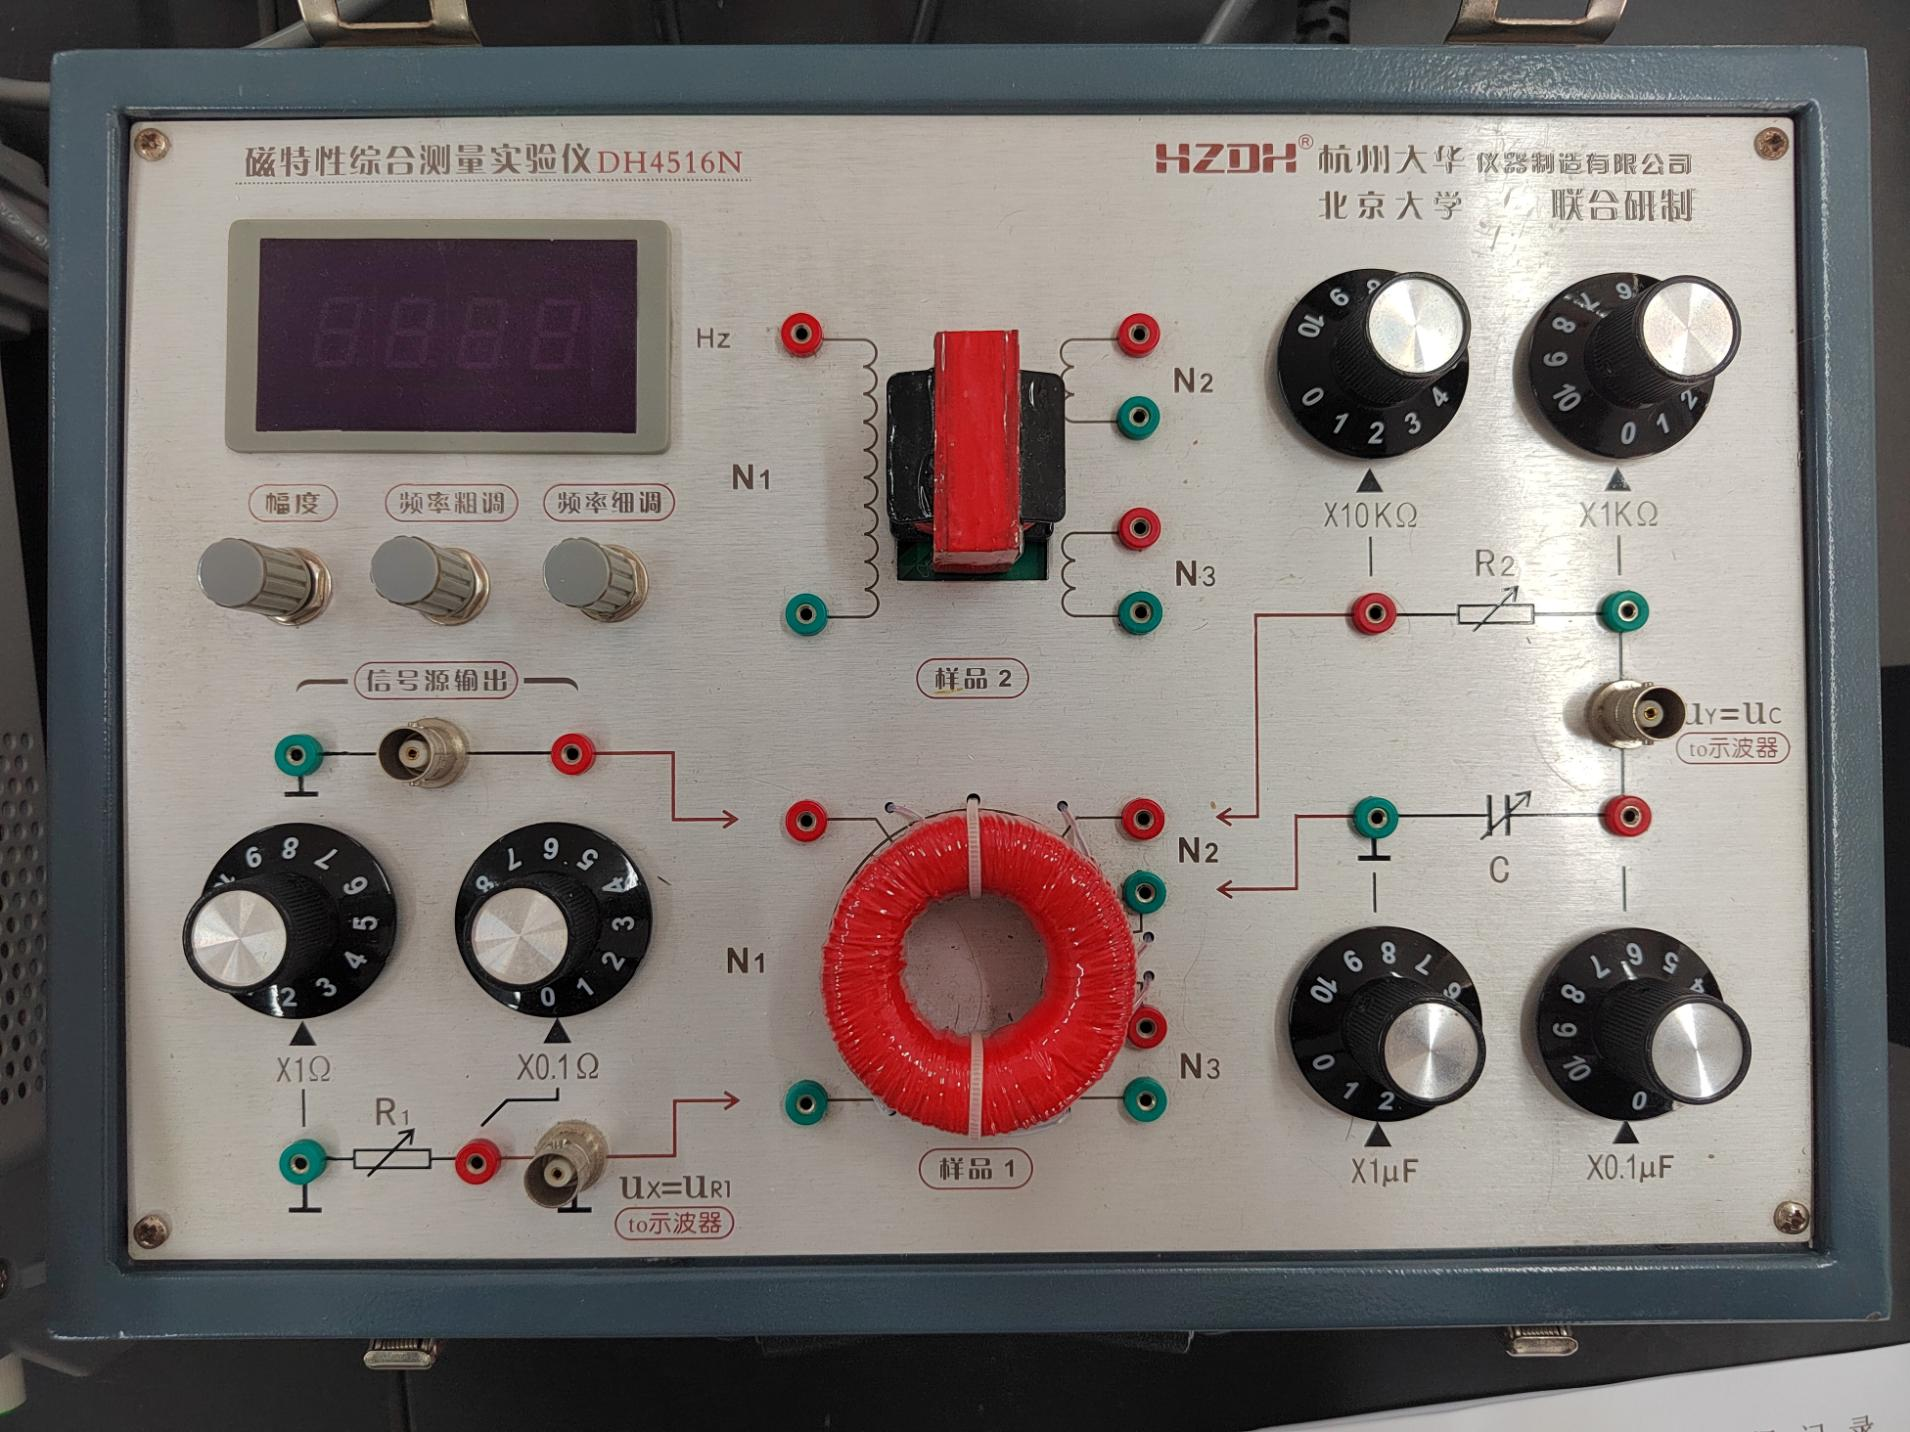
\includegraphics[height=170pt]{assets/DH4516 磁特性综合测量实验仪.jpg}
    \caption{DH4516 磁特性综合测量实验仪}
\end{subfigure}\hfill
\begin{subfigure}[b]{0.5\columnwidth}\centering
    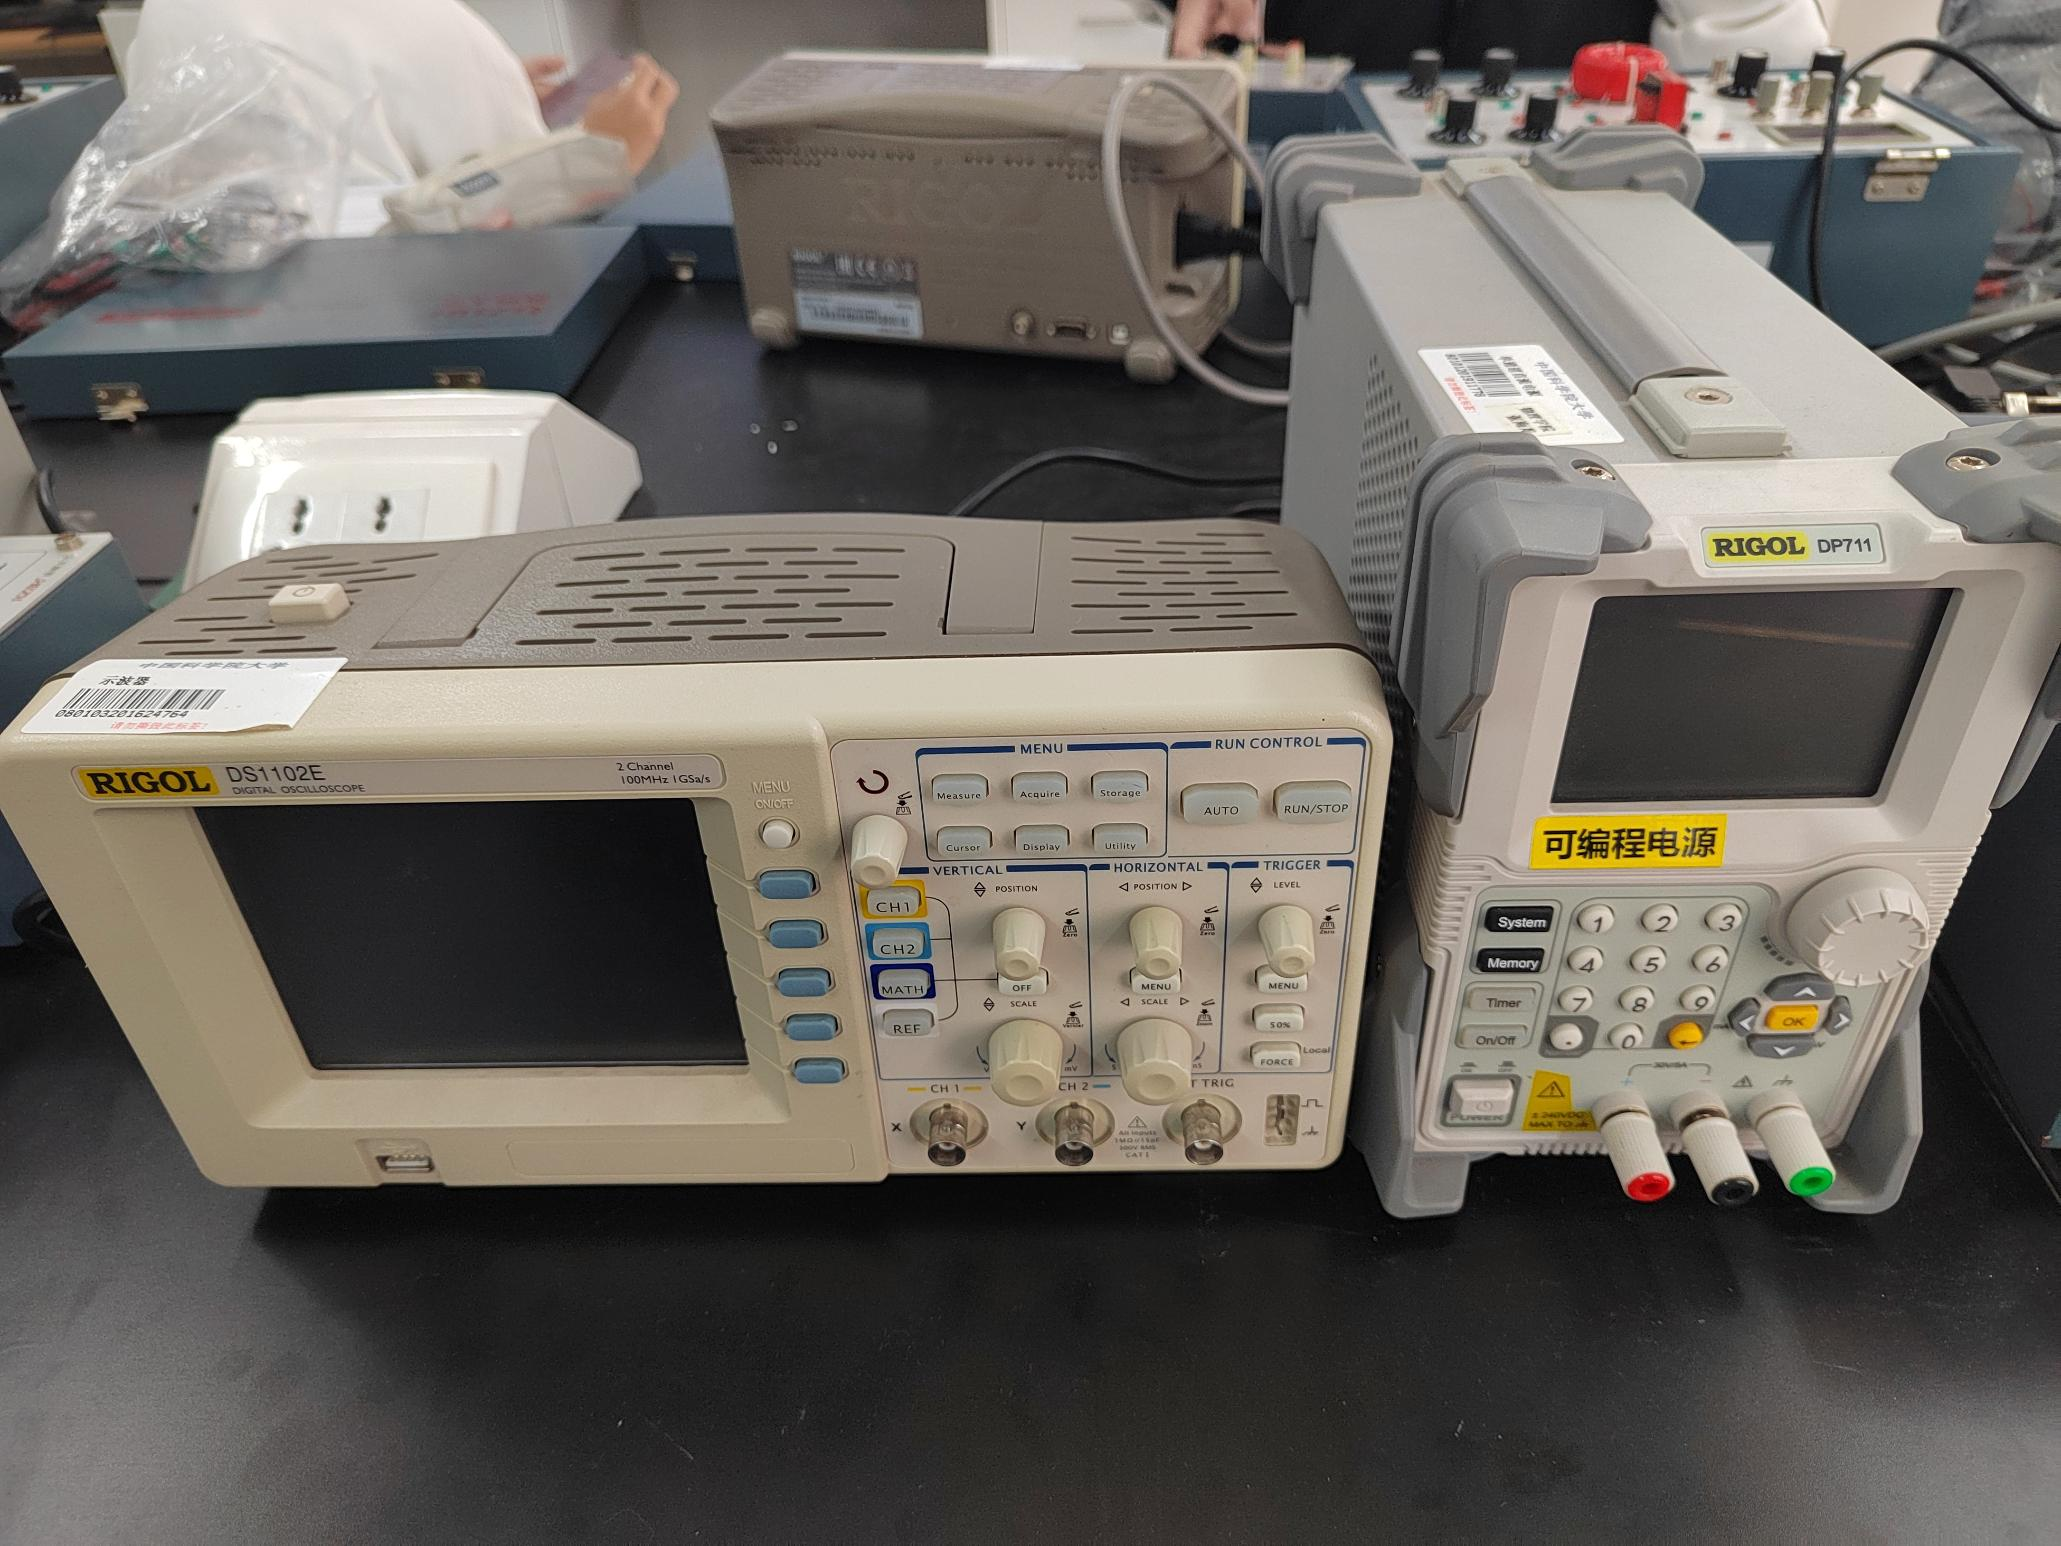
\includegraphics[height=170pt]{assets/示波器和可编程电源.jpg}
    \caption{双通道示波器和可编程电源}
\end{subfigure}
\caption{第一部分实验的主要实验仪器}
\end{figure}

另外,信号源的频率 $f$ 在 $ 20\ \mathrm{Hz} \sim 200\ \mathrm{Hz} $ 间可调;可调标准电阻 $ R_1,R_2 $ 均为线性无感交流电阻,$ R_1 $ 的调节范围为 $ 0.1 \ \Omega \sim 11\ \Omega $,$ R_2 $ 的调节范围为 $ 1 \kO \sim 100 \kO $;标准电容 $C$ 在 $ 0.1 \uF \sim 11 \uF $ 间可调。

\subsection{FD-BH-I 霍尔传感器磁滞回线和磁化曲线测定仪等}

FD-BH-I 霍尔传感器磁滞回线和磁化曲线测定仪(包括数字式特斯拉计、恒流源、磁性材料样品、磁化线圈、双刀双掷开关、霍耳探头移动架、双叉头连接线、箱式实验平台)。

其主要技术指标如下:
\begin{enumerate}
\item 数字式特斯拉计: 四位半LED 显示,量程 $0 \sim 2.000 $ T;分辨率 $0.1$ mT,带霍耳探头;
\item 恒流源:四位半 LED 显示,可调恒定电流 $0\sim 600.0$ mA;
\item 磁性材料样品:条状矩形结构,截面长 $2.00$ cm;宽 $2.00$ cm;间隙宽(隙隔) $l_g = 2.00$ mm;平均磁路长度 $l =0.240$ m(样品与固定螺丝为同种材料);
\item 磁化线圈总匝数 $N=2000$。
\end{enumerate}



\section{实验原理}
\subsection{铁磁材料的磁化特性}
把物体放在外磁场$ H $中,物体就会被磁化,在其内部产生磁场。设其内部磁化强度为$ M $,磁感应强度为$ B $,即可定义磁化率 $ \chi_m $ 和相对磁导率 $ \mu_r $: 
\begin{equation}
    \chi_m=\frac MH,\quad \mu_r=\frac{B}{\mu_0 H}
\end{equation}

其中$ \mu_0=4\pi\times10^{-7}\,\mathrm{N\cdot A^{-2}} $是真空磁导率。又由于 $ B=\mu_0(M+H) $,所以 $ \mu_r=1+\chi_m $。物质的磁性按磁化率可分为抗磁性($\chi_m < 0$)、顺磁性($\chi_m > 0$ 且较小)和铁磁性($\chi_m >0$ 且较大)三种,其中铁磁性物质的磁化率通常大于 1,远大于前两类物质。

除磁导率高这一特点外,铁磁材料还具有特殊的磁化规律。对一个处于磁中性状态(即完全退磁,外磁场 $H=0$ 时有 $B = 0$)的铁磁材料加上由小变大的磁场$ H $进行磁化时,磁感应强度$ B $随$ H $的变化曲线大致分为三个阶段:(1)可逆磁化阶段;(2)不可逆化阶段;(3)饱和磁化阶段。

如果磁场 $H$ 在某个范围 $ [-H_0,H_0] $ 间作循环变化,那么$ B $也会作循环变化,从而$ B-H $图像成为一个闭合的回线,称为磁滞回线。当 $H_0$ 比较大时,回线会有一段明显的饱和区(平稳区),此时得到的回线称为饱和磁滞回线,如图 \ref{铁磁材料的动态磁滞回线和动态磁化曲线示意图} 所示,$ H_S$ 和 $B_S $分别称为饱和磁场强度与饱和磁感应强度。

\begin{figure}[h]
    \centering
\resizebox{0.8\columnwidth}{!}{
    \begin{tikzpicture}
        \draw [->] (0,-4) -- (0,4);
        \draw [->] (-8,0) -- (8,0);
        \node [below] at (8,0) {$ H $};
        \node [left] at (0,4) {$ B $};
        \draw [thick] (-2,0) to [out=70,in=180] (5,3);
        \draw [thick] (-2,0) to [out=250,in=0] (-5,-3);
        \draw [thick] (-5,-3) to [out=0,in=250] (2,0);
        \draw [thick] (2,0) to [out=70,in=180] (5,3);
        \draw [thick] (5,3) -- (7.5,3);
        \draw [thick] (-5,-3) -- (-7.5,-3);
        \draw [dashed] (0,3) -- (5,3) -- (5,0);
        \node [left] at (0,3) {$ B_S $};
        \node [below] at (5,0) {$ H_S $};
        \draw [thick] (-1.5,-1.5) to [out=80,in=190] (1.5,1.5);
        \draw [thick] (-1.5,-1.5) to [out=10,in=260] (1.5,1.5);
        \draw [thick] (-0.7,-0.5) to [out=60,in=190] (0.7,0.5);
        \draw [thick] (-0.7,-0.5) to [out=10,in=240] (0.7,0.5);
        \draw [dashed] (0,0.5) -- (0.7,0.5) -- (0.7,0);
        \draw [dashed] (0,1.5) -- (1.5,1.5) -- (1.5,0);
        \node [left] at (0,2.3) {$ B_r $};
        \node [below] at (2.2,0) {$ H_C $};
        \node [left] at (0,1.5) {$ B_m $};
        \node [left] at (0,0.5) {$ B_{m'} $};
        \node [below] at (1.5,0) {$ H_m $};
        \node [below] at (0.7,0) {$ H_{m'} $};
        \draw [thick,dashed] (0,0) -- (0.2,0.1) to [out=30,in=240] (0.7,0.5) to [out=60,in=230] (1.5,1.5) to [out=50,in=180] (5,3);
    \end{tikzpicture}
}
    \caption{铁磁材料的动态磁滞回线和动态磁化曲线示意图}
    \label{铁磁材料的动态磁滞回线和动态磁化曲线示意图}
\end{figure}


同一频率下(动态磁滞回线的形状与磁化场频率与幅度都有关),将磁场幅值从0增到$ H_S $得到的一系列磁滞回线,他们的顶点$ (H_m,B_m) $的连线称为动态磁化曲线。从这条曲线出发,考虑足够弱的交流磁场、直流偏置磁场的情况,可以定义多种磁导率:
\begin{equation}
    \text{振幅磁导率\ } \mu_m=\frac{B_m}{\mu_0H_m},\quad
    \text{起始磁导率\ } \mu_i=\lim_{H\to0}\frac{B}{\mu_0H},\quad
    \text{可逆磁导率\ } \mu_R=\lim_{\Delta H\to 0}\frac{\Delta B}{\mu_0\Delta H}
\end{equation}
其中 $\Delta B$,$\Delta H$ 分别是交流弱磁场引起的磁感应强度变化值和磁场强度变化值,可调电源带来的直流偏置仅是为交流电路设定工作点。

闭合磁滞回线的面积 $A$ 对应于循环磁化一周所发生的能量损耗 $-\Delta E$。对材料进行交流动态磁化时,损耗来自于磁滞损耗、涡流损耗、剩余损耗。对于金属氧化物组成的铁氧体磁性材料电阻率高,高频条件下其涡流损耗很小。

由于铁磁材料在加上磁场$ H $后产生的$ B $不仅与磁场强度本身有关,还与材料的磁化历史有关,所以在研究铁磁材料的起始磁化性质时,通常需要对铁磁材料进行退磁处理,使之达到磁中性状态。

\subsection{动态磁滞回线的测量}
测量动态磁滞回线的原理电路如图 \ref{用示波器测量动态磁滞回线电路图} 所示。环形铁芯上绕有三组线圈。线圈 1 为交流励磁线圈,接交流正弦信号源;线圈 2 为感应线圈,接 RC 积分电路;线圈 3 为直流励磁线圈,用于在测有直流偏置磁场下的可逆磁导率时接直流电源。将$ u_{R_1} $和$ u_C $从示波器两通道输入,在示波器 X-Y 显示模式下即可看到动态磁滞回线。

下面推导图 \ref{用示波器测量动态磁滞回线电路图} 装置的理论原理。设 $i_1$、$i_2$ 分别是线圈 1、线圈 2 中的电流, $ N_1 $、$N_2$、$N_3$ 分别是线圈1、线圈2、线圈3的匝数,$ l $是磁环的等效磁路长度,$ \Phi $是单匝线圈中的磁通量,$ S $是单匝线圈环绕的面积(相当于磁芯的横截面积),$T$ 为交流激励(外磁场)的周期。由安培环路定理和法拉第电磁感应定律,我们有:
\begin{gather}
H = \frac{N_1}{l}i_1 = \frac{N_1}{lR_1}\cdot u_{R_1} \Longrightarrow \boxed{
    H = \frac{N_1}{lR_1}\cdot u_{R_1} \propto u_{R_1}
} 
\\ 
u_2 = - N_2 \frac{\mathrm{d} \Phi }{\mathrm{d} t } = - N_2S \frac{\mathrm{d} B }{\mathrm{d} t } 
\\ 
u_C = \frac{Q}{C} = u_C|_{t = 0} + \frac{1}{CR_2} \int_{0}^{t} u_{R_2}\mathrm{d}t \approx \frac{1}{CR_2} \int_{0}^{t} u_{R_2}\mathrm{d}t \quad  (R_2 C \gg T) 
\\
\Longrightarrow \boxed{
    B = \frac{R_2 C}{N_2 S}\cdot u_C \propto u_C
}
\end{gather}

因此,只需利用双通道示波器对 $u_{R_1}$ 和 $u_C$ 进行测量,便和等价地得到 $H$ 和 $B$,进而绘制出 $H$-$B$ 图像,得到动态磁化曲线或磁滞回线。

\begin{center}\noindent\begin{minipage}{0.48\columnwidth}
\begin{figure}[H]\centering
    \resizebox{!}{150pt}{
        \begin{circuitikz}
            \draw (0,0) 
            to[sinusoidal voltage source] (0,2)
            to[short,-.] (2,2);
            \draw (4.5,1) circle [radius=2];
            \draw (4.5,1) circle [radius=2.5];
            \draw (0,0) to[european resistor,l=$ R_1 $,a=CH1,-.] (2,0);
            \draw (0,-0.1) -- (0,-0.9);
            \draw (2,-0.1) -- (2,-0.9);
            \draw [<-](0,-0.55)--(0.5,-0.55);
            \draw [->](1.5,-0.55)--(2,-0.55);
            \draw (2,2) to [out=0,in=20] (2.6,1.6);
            \draw (2.05,1.45) to[out=175,in=10] (2.5,1);
            \draw (2.015,0.8) to[out=190,in=30] (2.6,0.4);
            \draw (2,0) to[out=0,in=220] (2.14,0.14);
            \node [left] at (2,1) {$ N_1 $};
            
            \draw (7,2)
            to[short,.-] (9,2)
            to[european resistor,l=$ R_2 $] (9,0)
            to[C,l_=$ C $,a^=CH2] (7,0);
            \draw [<-](7,-0.65)--(7.5,-0.65);
            \draw [->](8.5,-0.65)--(9,-0.65);
            \draw (7,-0.1)--(7,-1.1);
            \draw (9,-0.1)--(9,-1.1);
            \draw (7,2) to[out=180,in=150] (6.37,1.7);
            \draw (6.97,1.4) to[out=340,in=150] (6.5,1);
            \draw (6.97,0.6) to[out=340,in=150] (6.37,0.3);
            \draw (7,0) to[out=180,in=330] (6.83,0.1);
            \node [right] at (7,1) {$ N_2 $};
            
            \draw (3,3.5)
            to[short] (3,4)
            to[ammeter,-.] (4.5,4);
            \draw (6,5)
            to[american inductor] (6,3.5);
            \draw (6,5)
            to[european potentiometer,*-] (3,5)
            to[short] (3,6)
            to[battery] (6,6)
            to[short] (6,5);
            \draw [thick] (4.5,4) -- (4.5,4.5);
            \draw (3,3.5) to[out=270,in=250] (3.45,2.7);
            \draw (3.6,3.33) to[out=75,in=245] (4,2.93);
            \draw (4.2,3.48) to[out=80,in=230] (4.6,2.99);
            \draw (4.9,3.47) to[out=50,in=240] (5.2,2.88);
            \draw (5.4,3.342) to[out=60,in=240] (5.6,2.66);
            \draw (6,3.5) to[out=270,in=60] (5.85,3.1);
            \node [below] at (4.5,2.5) {$ N_3 $};
        \end{circuitikz}
    }
    \caption{用示波器测量动态磁滞回线电路图}
    \label{用示波器测量动态磁滞回线电路图}
\end{figure}
\end{minipage}\hfill\begin{minipage}{0.51\columnwidth}
\begin{figure}[H]\centering
    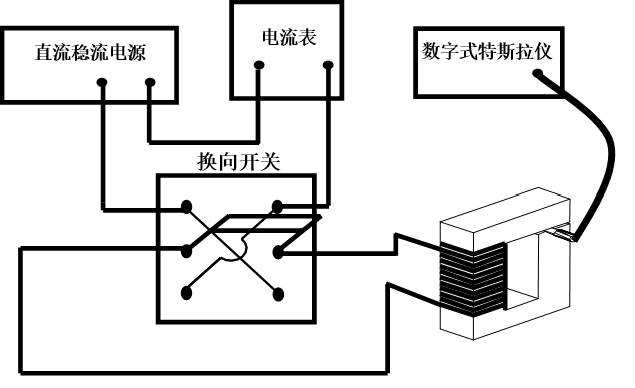
\includegraphics[height=150pt]{assets/磁滞回线和磁化曲线的霍尔测量装置.png}
\caption{磁滞回线和磁化曲线的霍尔测量装置}\label{磁滞回线和磁化曲线的霍尔测量装置}
\end{figure}
\end{minipage}\end{center}



\subsection{(准)静态磁化曲线和(准)静态磁滞回线的测量}

实验装置如图 \ref{磁滞回线和磁化曲线的霍尔测量装置} 所示。经过“磁锻炼”之后,设测得环形样品的磁化线圈中通过的电流为 $I$,则磁化场的磁场强度 $H$ 为:
\begin{equation}
    \boxed{
        H = \frac{N}{l}I
    }
\end{equation}
其中 $N$ 为磁化线圈的匝数, $l$ 为样品平均磁路长度, $H$ 的单位为A/m。而实际测量中,需要对 $H$ 进行修正,由:
\begin{equation}
    Hl + H_g l_g = NI ,\quad B = \mu_0\mu_rH_g ,\quad \mu_r = 1
\end{equation}
可以得到修正后的磁场强度值,记作 $H_{\text{revised}}$,或简记为 $H_{\text{re}}$:
\begin{equation}
    \boxed{
        H_{\text{re}} = \frac{N}{l}I-\frac{l_g}{\mu_0l}B
    }
\end{equation}


\section{实验内容与步骤}

\subsection{第一部分}

\subsubsection{实验一:观测样品 1(铁氧体)的饱和动态磁滞回线}
根据原理电路图连接样品 1 与交流励磁电路、RC积分电路,如图 \ref{第一部分实验一接线图} 所示。

\begin{enumerate}
\item 调节频率为$ f=100\,\mathrm{Hz} $,取参数$ R_1=2.0\,\Omega $,$ R_2=50\,\mathrm k\Omega $,$ C=10.0\,\mu\mathrm F $。调节励磁电流大小与示波器,用示波器的X-Y模式观察$ u_C-u_{R_1} $图像,由于$ B\propto u_C,\,H\propto u_{R_1} $,所观察到的图像即为在X,Y方向缩放后的磁滞回线。调得相对原点对称的饱和磁滞回线,利用示波器光标(cursor)功能测量$ B_S,B_r,H_C $,并在图像的上下半支各取不少于 9 个数据点进行记录,即 9 个横坐标 $H$,9 对纵坐标 $(B_1, B_2)$。根据所取的数据点绘制磁滞回线的$ B-H $图像。
\item 在同一幅度下,在仪器频率可调范围内,观测不同频率时的磁滞回线。特别地,在$ R_1,R_2C $不变时测量并比较$ f=95\,\mathrm{Hz} $和$ 150\,\mathrm{Hz} $时的$ B_r $与$ H_C $。
\item 在频率$ f=50\,\mathrm{Hz} $下,固定励磁电流幅度$ I_m=0.1\,\mathrm A $,$ R_1=2.0\,\Omega $,改变积分常量$ R_2C $分别为$ 0.01\,\mathrm s,\;0.05\,\mathrm s,\;0.5\,\mathrm s $,观察并粗略绘制不同积分常量下$ u_{R_1}-u_C $李萨如图形的示意图,并考虑积分常量为何影响该李萨如图形,是否影响真实的磁滞回线形状?
\end{enumerate}

\begin{figure}[H]\centering
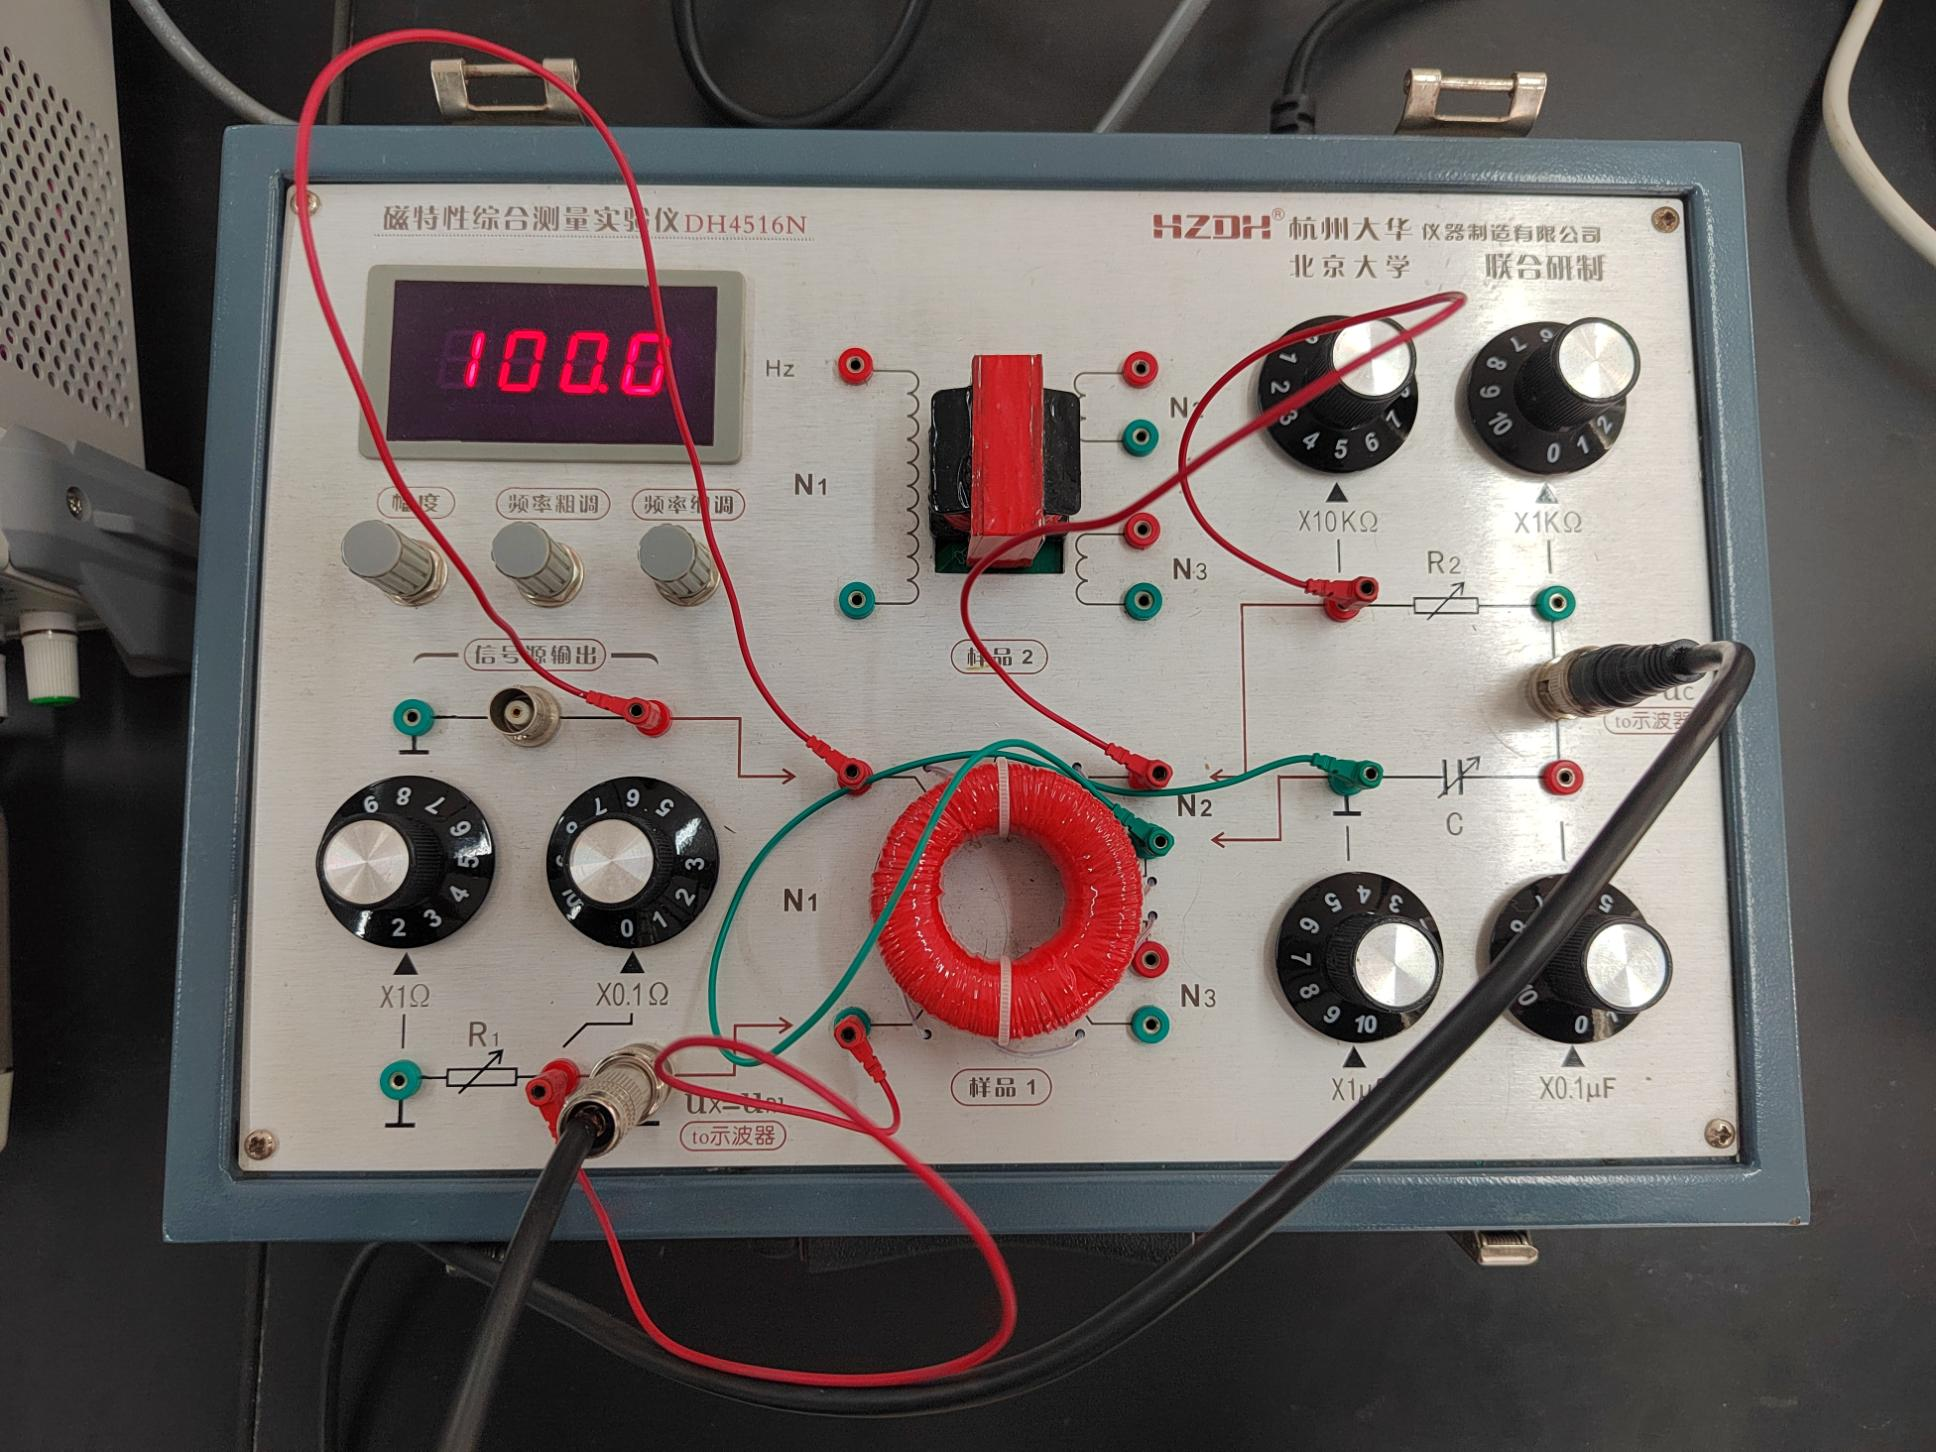
\includegraphics[width=0.6\columnwidth]{assets/1.1/第一部分实验一接线图.jpg}
\caption{第一部分实验一接线图}\label{第一部分实验一接线图}
\end{figure}

\subsubsection{实验二:测量样品 1(铁氧体)的动态磁化曲线}

\begin{enumerate}
\item 在$ f=100\,\mathrm{Hz} $时,取$ R_1=2.0\,\Omega $,$ R_2=50\,\mathrm k\Omega $,$ C=10.0\,\mu\mathrm F $,调节磁场幅度从$ 0 $单调增加到$ H_S $,取至少二十个数据点,并绘制动态磁化曲线。
\item 根据测得数据,计算并画出$ \mu_m-H_m $曲线。
\item 测定起始磁导率$ \mu_i $;
\end{enumerate}


\subsubsection{实验三:观察不同频率下样品 2(硅钢)的动态磁滞回线}

改变电路连接方式,将样品 2 接入实验电路。然后取$ R_1=2.0\,\Omega $,$ R_2=50\,\mathrm k\Omega $,$ C=10.0\,\mu\mathrm F $,给定交变磁场幅度$ H_m=400\,\mathrm{A/m} $下,分别测量频率$ f=20\,\mathrm{Hz},\;40\,\mathrm{Hz},\;60\,\mathrm{Hz} $时的$ B_m,\,B_r,\,H_C $。

\subsubsection{实验四:测量样品 1(铁氧体)在不同直流偏置磁场下的可逆磁导率}
改变电路连接方式,重新将样品 1 接入电路,对其进行退磁处理,并将直流偏置电路与对应线圈连通。然后设置交流磁场频率为$ f=100\,\mathrm{Hz} $,其幅度$ \Delta H $足够小,调节电阻、电容分别为$ R_1=2.0\,\Omega,\;R_2=20\,\mathrm k\Omega,\;C=2.0\,\mu\mathrm F $。将直流偏置磁场从0单调增加到$ H_S $,调节示波器使得便于观察磁化的可逆过程,记录至少10个不同$ H $下的磁导率$ \mu_R $,绘制$ \mu_R-H $曲线。


\subsection{第二部分}

\subsubsection{实验一:测量模具钢的(准)静态起始磁化曲线}

将霍尔传感器置于磁场中央,取 14 个采样点,调整直流偏置磁场的大小,测量样品的起始磁化曲线,并利用测得的 $B$ 和修正后的磁场强度 $H_{\text{re}}$ 作图。

\subsubsection{实验二:测量模具钢的(准)静态磁滞回线}

对样品进行磁锻炼后,将磁化线圈的电流从最大电流 $I_m$ 开始,逐步减小到 0,然后由 0 反向增大至 $-I_m$,重复上述过程,直至回到 $I_m$。每隔 50 mA 测一组 $(I, B)$ 值。最后利用测得的 $B$ 和修正后的磁场强度 $H_{\text{re}}$ 作图。

\newpage
\section{实验结果与数据处理}

下面是数据处理需要用到的公式,在此一并列出:
\begin{align}
\boxed{
\begin{aligned}
    \text{第一部分中 $H$ 和 $B$ 的测量原理:}& H = \frac{N_1}{l_{1, k}R_1}\cdot u_{R_1},\quad B = \frac{R_2 C}{N_2 S_k}\cdot u_C
    \\
    \text{直流偏置下的测量原理:}&  H = \frac{N_3}{l_{1, k}}\cdot I,\quad \mu_R=\lim_{\Delta H\to 0}\frac{\Delta B}{\mu_0\Delta H}
    \\
    \text{第二部分中 $H$ 和 $H_{\text{re}}$ 的测量原理:}& H = \frac{N}{l_2}\cdot I,\quad H_{\text{re}} = \frac{N}{l_2}\cdot I - \frac{l_g}{\mu_0 l_2}\cdot B
\end{aligned}
}
\end{align}
实验中可能需要的常量如下所示:
\begin{gather}
    \mu_0 = 4\pi \times 10^{-7}\  \mathrm{H\cdot m},\ \ 
    l_{1, 1} = 0.13 \ \mathrm{m},\ \ 
    l_{1, 2} = 0.075 \ \mathrm{m}
    \\
    S_1 = 1.24 \times 10^{-4}\ \mathrm{m^2} ,\ \ 
    S_2 = 1.20 \times 10^{-4}\ \mathrm{m^2} ,\ \ 
    N_k = 150
    \\ 
    l_2 = 0.240 \ \mathrm{m},\ \ l_g = 2 \times 10^{-3} \ \mathrm{m},\ \ N = 2000
\end{gather}

对于每个小实验,我们会将对应的参数列出,给出具体的数据换算公式,然后代入计算。

\subsection{第一部分}
\subsubsection{实验一:观测样品 1(铁氧体)的饱和动态磁滞回线}\label{铁氧体}

\noindent \textbf{(1)} 本节我们使用样品 1,参数 $f = 100 \ \mathrm{Hz}$,$R_1 = 2.0 \ \Omega$,$R_2 = 50.0 \kO$,$C = 10 \uF$,于是有换算公式 (\ref{1.1换算公式})。我们共测得 13 个数据点,原始电压测量结果见表 \ref{1.1电压},换算结果见表 \ref{1.1换算后}。

\begin{equation}\label{1.1换算公式}
    H = \frac{N_1}{l_{1, 1}R_1}\cdot u_{R_1} = 576.9231\  u_{R_1},\quad 
    B = \frac{R_2 C}{N_2 S_1}\cdot u_C = 26.8817 \ u_C
\end{equation}

\begin{center}\noindent\begin{minipage}{0.35\columnwidth}
\begin{table}[H]\centering
        %\renewcommand{\arraystretch}{1.5} % 调整行间距为 1.5 倍
        %\setlength{\tabcolsep}{1.5mm} % 调整列间距
        \caption{原始电压数据点}
        \label{1.1电压}
    \begin{tabular}{cccccccccc}\toprule
$u_{R_1}$ (mV) & $u_{C, 1}$ (mV) & $u_{C, 2}$ (mV)  \\
\midrule
-456  & -22.0 & -22.0 \\
-228  & -21.6 & -21.6 \\
-91.2 & -19.2 & -19.2 \\
-45.6 & -15.6 & -17.2 \\
-22.8 & -9.20 & -14.0 \\
-6.60 & 0.00  & -10.0 \\
0.00  & 4.00  & -7.60 \\
13.2  & 8.80  & 0.00  \\
22.2  & 10.8  & 5.60  \\
44.4  & 14.8  & 12.8  \\
88.8  & 17.6  & 17.6  \\
222   & 20.0  & 20.0  \\
444   & 20.8  & 20.8  \\
        \bottomrule
    \end{tabular}
\end{table}
\end{minipage}\begin{minipage}{0.35\columnwidth}
\begin{table}[H]\centering
    %\renewcommand{\arraystretch}{1.5} % 调整行间距为 1.5 倍
    %\setlength{\tabcolsep}{1.5mm} % 调整列间距
    \caption{换算后的磁滞回线数据点}
    \label{1.1换算后}
    \begin{tabular}{ccc}\toprule
$H$ $\mathrm{(A\cdot m^{-1})}$ & $B_1$ (T) & $B_2$ (T)  \\
\midrule
-263.077 &-0.591 &-0.591 \\
-131.538 &-0.581 &-0.581 \\
-52.615	 &-0.516 &-0.516 \\
-26.308	 &-0.419 &-0.462 \\
-13.154	 &-0.247 &-0.376 \\
-3.808	 &0.000	 &-0.269 \\
0.000	 &0.108	 &-0.204 \\
7.615	 &0.237	 &0.000  \\
12.808	 &0.290	 &0.151  \\
25.615	 &0.398	 &0.344  \\
51.231	 &0.473	 &0.473  \\
128.077	 &0.538	 &0.538  \\
256.154	 &0.559	 &0.559  \\
\bottomrule
    \end{tabular}
\end{table}
\end{minipage}
\begin{minipage}{0.24\columnwidth}
\begin{figure}[H]\centering
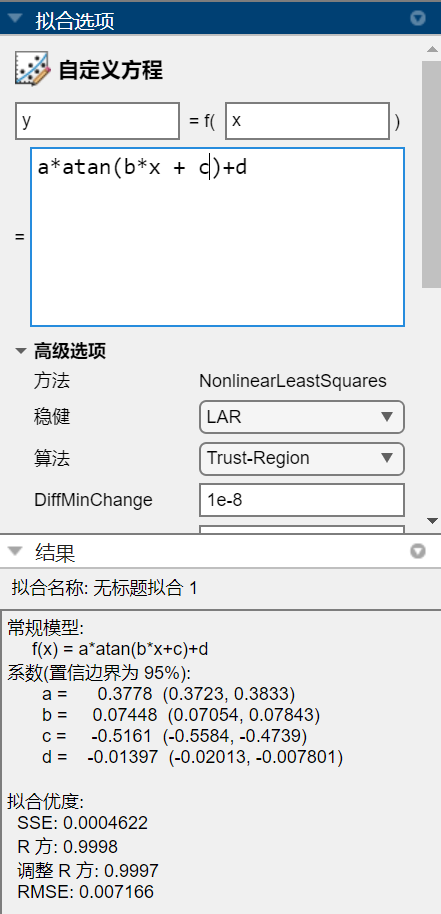
\includegraphics[width=\columnwidth]{assets/1.1/(1)/下半支.png}
\caption{拟合结果与优度}\label{1.1拟合优度}
\end{figure}
\end{minipage}
\end{center}


为了得到较准确的 $B_r$ 和矫顽力 $H_c$,我们利用 Matlab 软件对数据进行拟合,定义拟合函数为:
\begin{equation}
y = f(x) = a \arctan (b x + c) + d
\end{equation}
其中 $a, b, c, d$ 为待定常数。据此拟合磁滞回线的半支,拟合两次分别得到上下半支。拟合优度如图 \ref{1.1拟合优度} 所示。

依据原始数据和拟合结果,作出动态磁滞回线,如图 \ref{1.1图} 所示\footnote{Matlab 源码见附录 \ref{1.1源码}}。实验时的实际图像如图 \ref{1.1照片} 所示,结合优度参数和拟合图像,可以知道拟合效果极好,于是由此拟合结果可得 $B_r$ 和 $H_c$ :
\begin{equation}
    B_r = 0.13707 \ \mathrm{T}\quad ,\quad H_c = 5.2432 \ \mathrm{A\cdot m^{-1}}\quad
\end{equation}

\begin{figure}[H]\centering
\begin{subfigure}[b]{0.5\columnwidth}\centering
    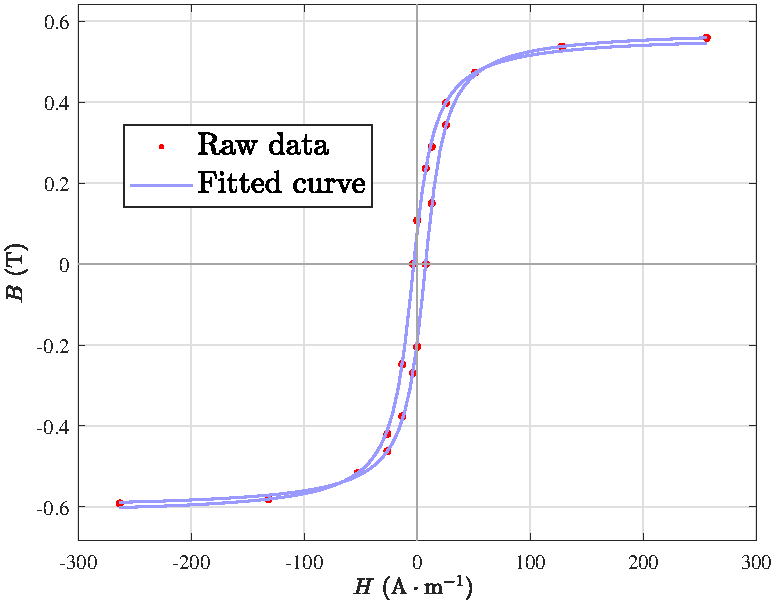
\includegraphics[height=190pt]{assets/1.1/(1)/2024-10-23_01-06-12.pdf}
    \caption{饱和磁滞回线}
\end{subfigure}\hfill
\begin{subfigure}[b]{0.5\columnwidth}\centering
    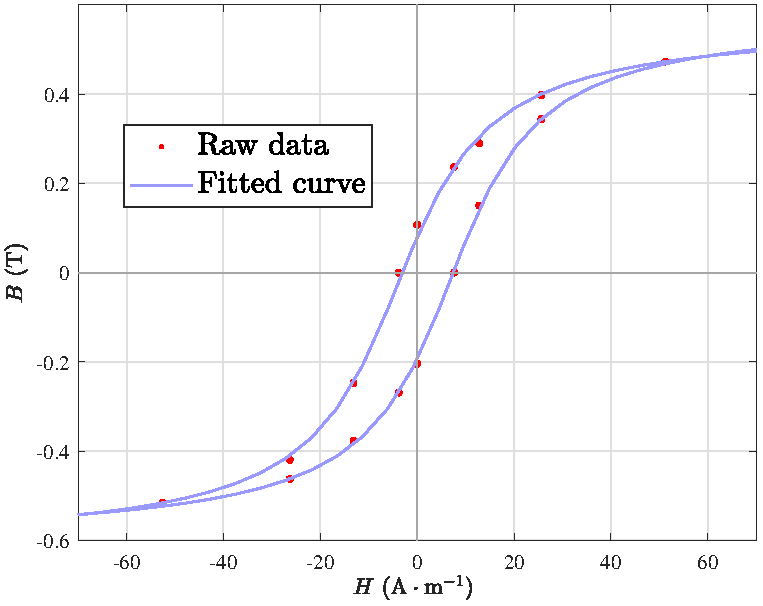
\includegraphics[height=190pt]{assets/1.1/(1)/2024-10-23_01-06-14.pdf}
    \caption{局部放大图}
\end{subfigure}
\caption{磁感应强度 $B$ 随外磁场 $H$ 的变化情况}
\label{1.1图}
\end{figure}
\begin{figure}[H]\centering
\begin{subfigure}[b]{0.5\columnwidth}\centering
    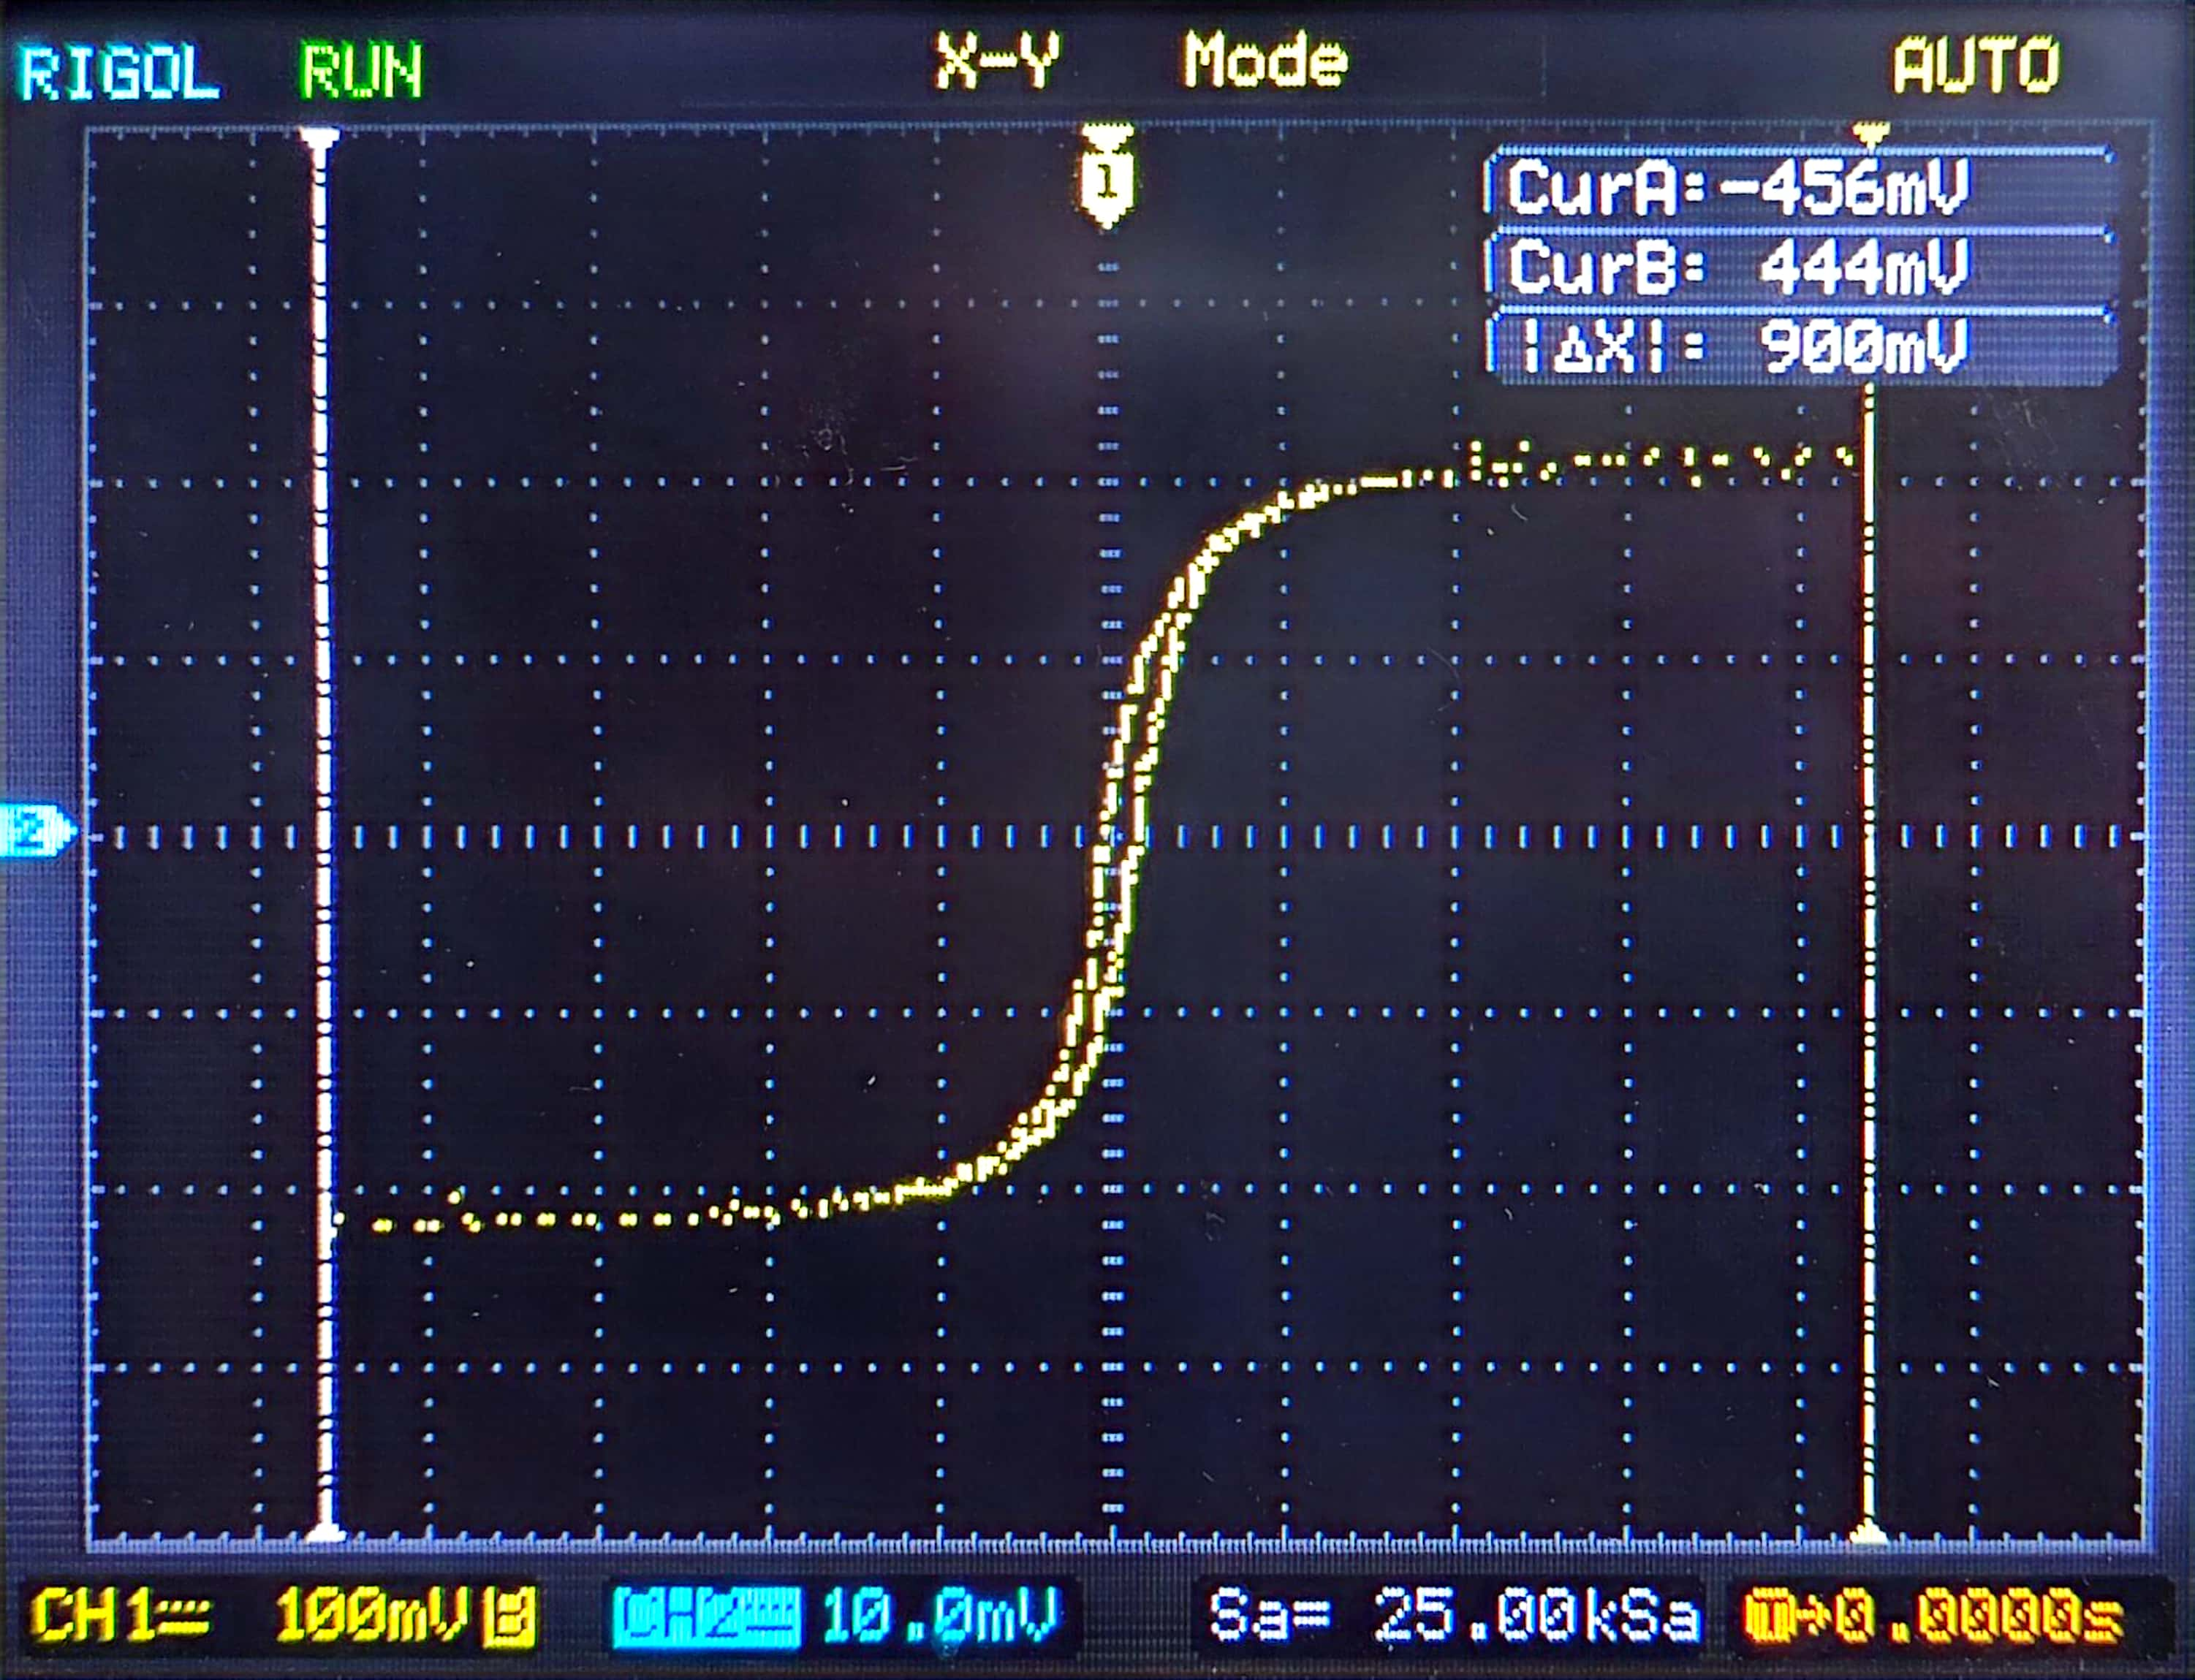
\includegraphics[height=170pt]{assets/1.1/(1)/CamScanner 10-22-2024 18.26_06.jpg}
    \caption{饱和磁滞回线}
\end{subfigure}\hfill
\begin{subfigure}[b]{0.5\columnwidth}\centering
    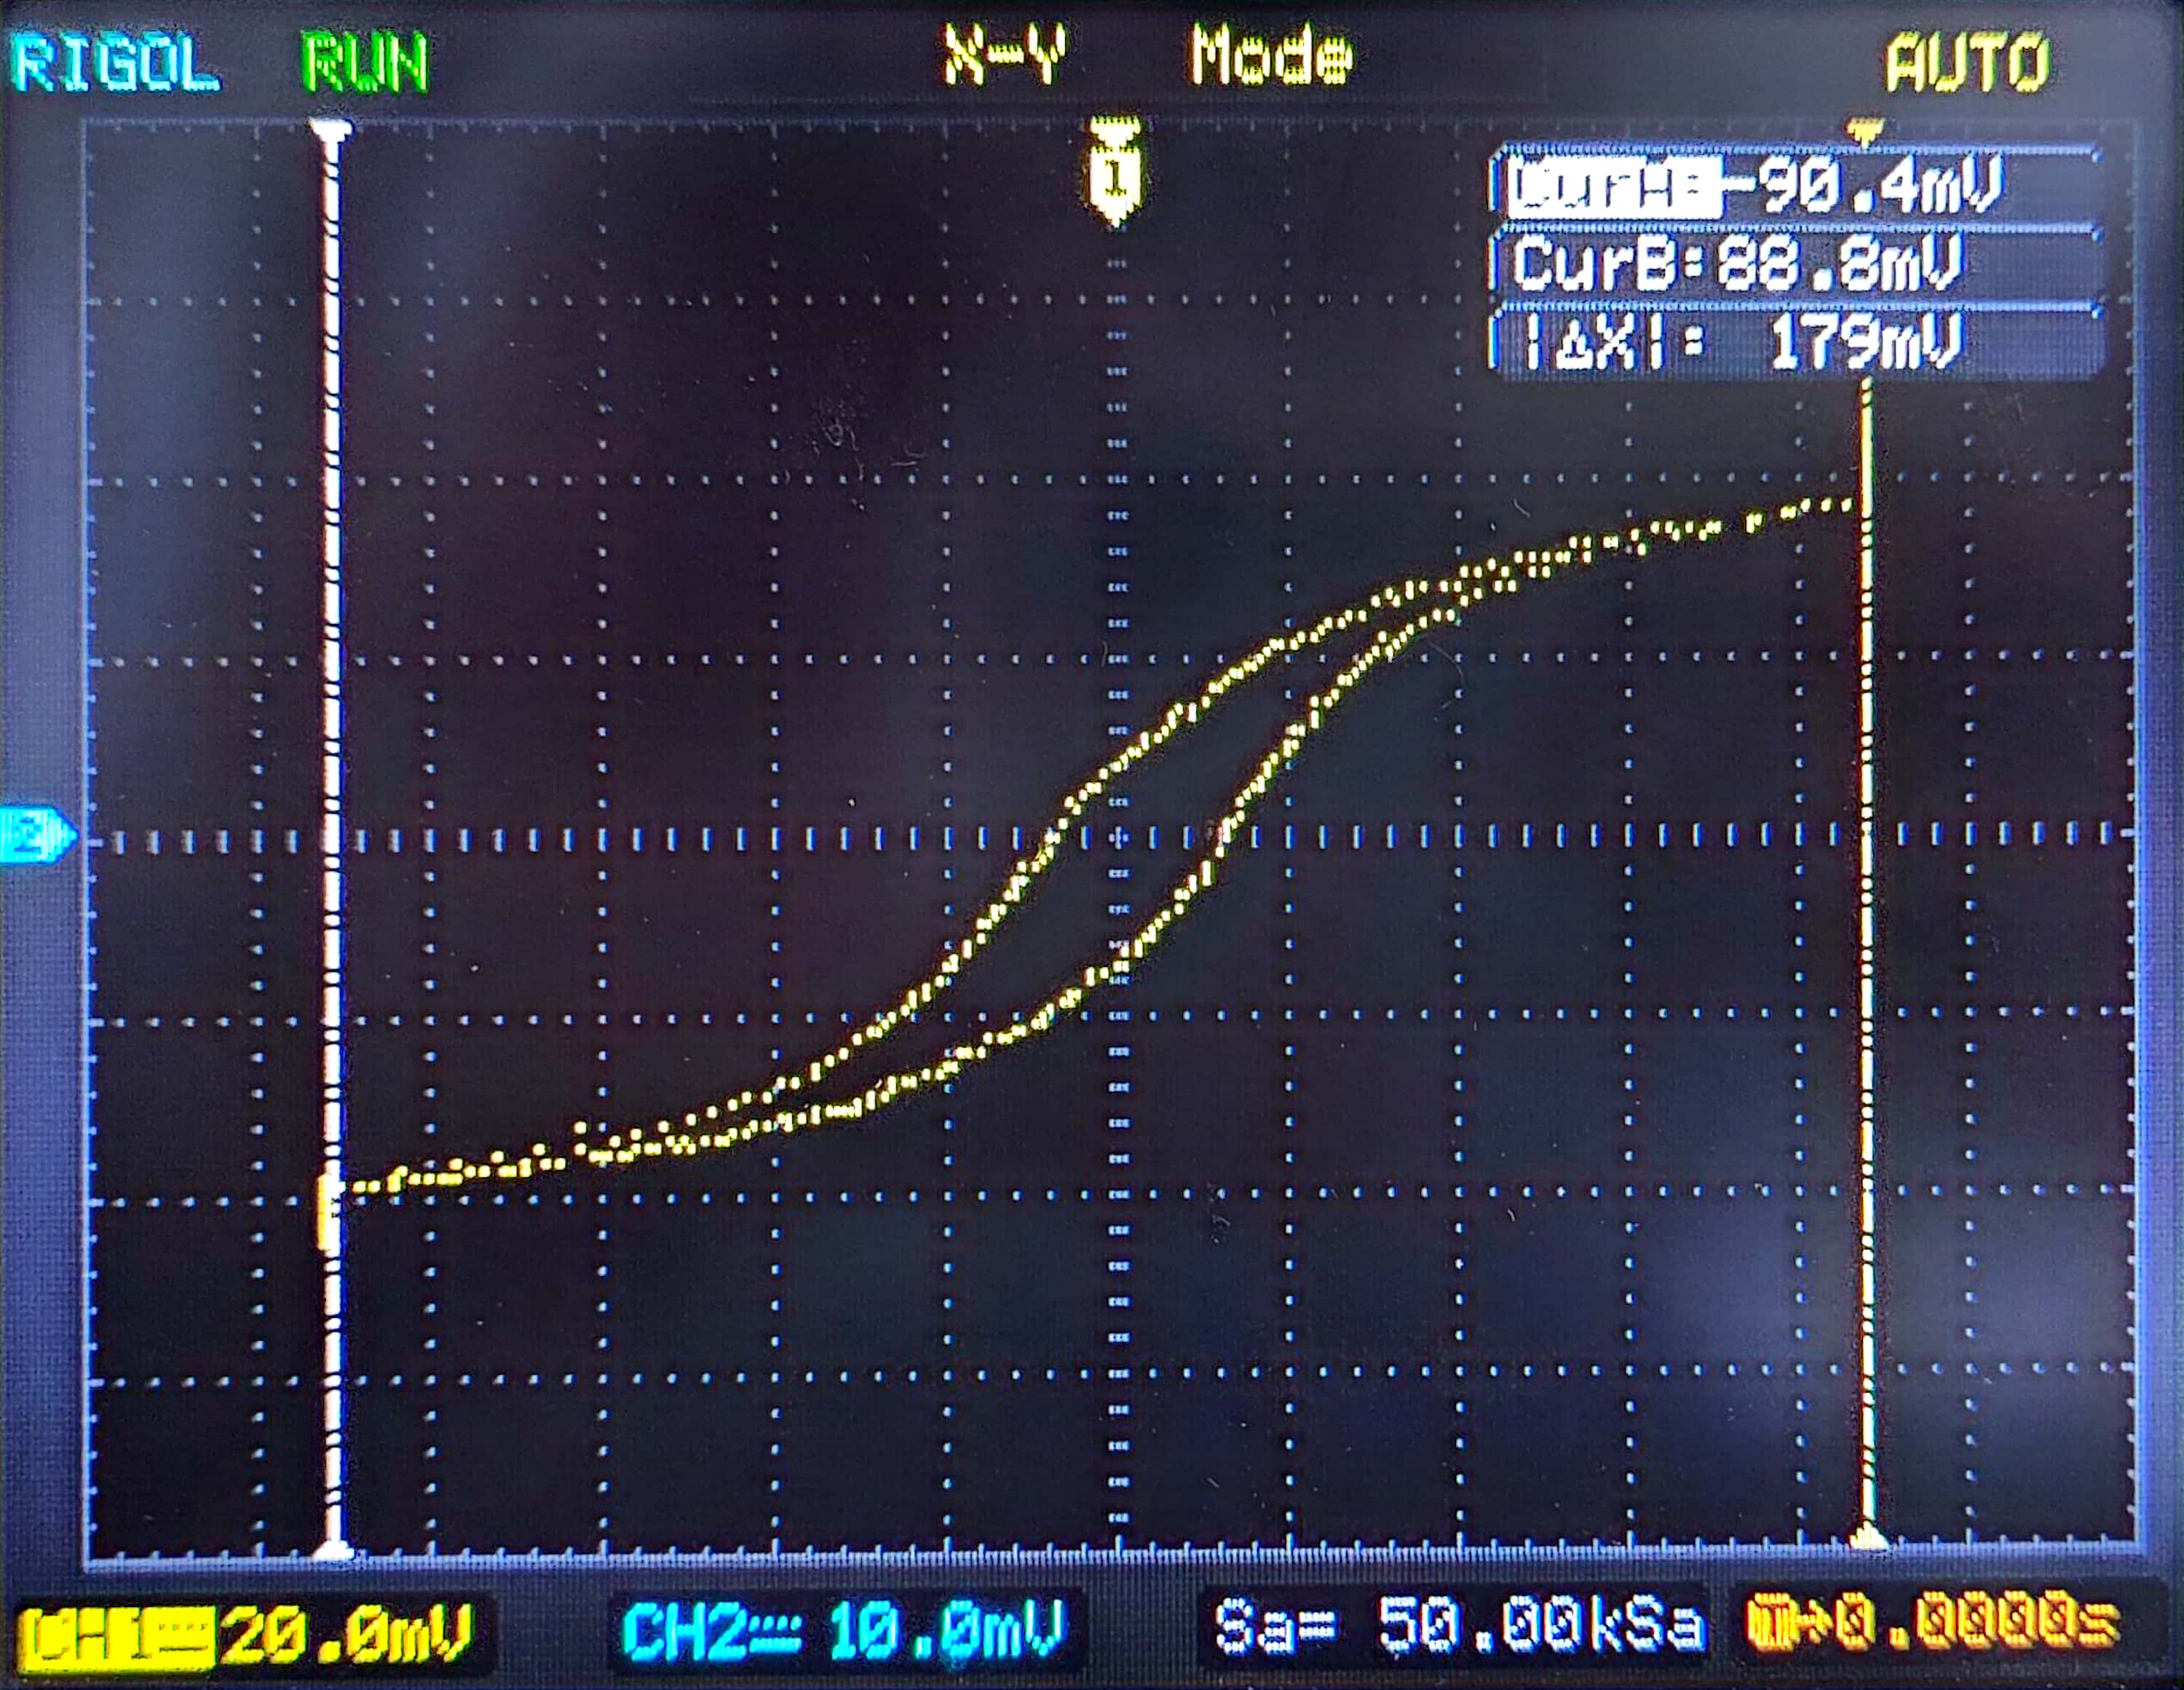
\includegraphics[height=170pt]{assets/1.1/(1)/CamScanner 10-22-2024 18.26_08.jpg}
    \caption{局部放大图}
\end{subfigure}
\caption{磁感应强度 $B$ 随外磁场 $H$ 的变化情况 (实物图)}\label{1.1照片}
\end{figure}

\noindent \textbf{(2)} 仍利用公式 (\ref{1.1换算公式}) 进行数值换算,得到不同频率时的 $B_r$ 和 $H_c$,结果如下表所示:

\begin{center}
    \noindent\begin{minipage}{0.49\columnwidth}
    \begin{table}[H]\centering
        %\renewcommand{\arraystretch}{1.5} % 调整行间距为 1.5 倍
        %\setlength{\tabcolsep}{1.5mm} % 调整列间距
        \caption{原始电压数据}
    \begin{tabular}{cccccccccc}\toprule
        $f$ (Hz) & $B_r$ (T) & $H_c \ \mathrm{A\cdot m^{-1}}$  \\
        \midrule
        95  & 5.80 & 10.2  \\
        100 & 5.10 & 9.10  \\
        150 & 4.40 & 7.60 \\
        \bottomrule
    \end{tabular}
    \end{table}
\end{minipage}\begin{minipage}{0.49\columnwidth}
    \begin{table}[H]\centering
        %\renewcommand{\arraystretch}{1.5} % 调整行间距为 1.5 倍
        %\setlength{\tabcolsep}{1.5mm} % 调整列间距
        \caption{不同频率时的 $B_r$ 和 $H_c$}
    \begin{tabular}{cccccccccc}\toprule
        $f$ (Hz) & $B_r$ (T) & $H_c \ \mathrm{A\cdot m^{-1}}$  \\
        \midrule
        95  & 0.1559 & 5.8846  \\
        100 & 0.1371 & 5.2432  \\
        150 & 0.1183 & 4.3846  \\
        \bottomrule
    \end{tabular}
    \end{table}
\end{minipage}
\end{center}


可以看到,在信号源幅度保持不变的情况下,频率越高,$B_r$ 和 $H_c$ 值越小,饱和磁滞回线所围成的面积越小。

这是因为,属于金属氧化物的锰锌铁氧体电阻率较高,交变磁场频率增大时,其涡流损耗变小,交变磁场磁化过程中的总能量损耗减小,而饱和磁滞回线所包围的面积正比于该损耗,所以饱和磁滞回线所包围的面积减小。

这是因为,属于金属氧化物的锰锌铁氧体电阻率较高,交变磁场频率增大时,其涡流损耗变小,交变磁场磁化过程中的总能量损耗减小,而饱和磁滞回线所包围的面积正比于该损耗,所以饱和磁滞回线所包围的面积减小。

\noindent \textbf{(3)} 改变积分常量 $R_2 C$,得到不同积分常量下的李萨如图形(动态磁滞回线),如下所示:
\begin{figure}[H]\centering
\begin{subfigure}[b]{0.33\columnwidth}\centering
    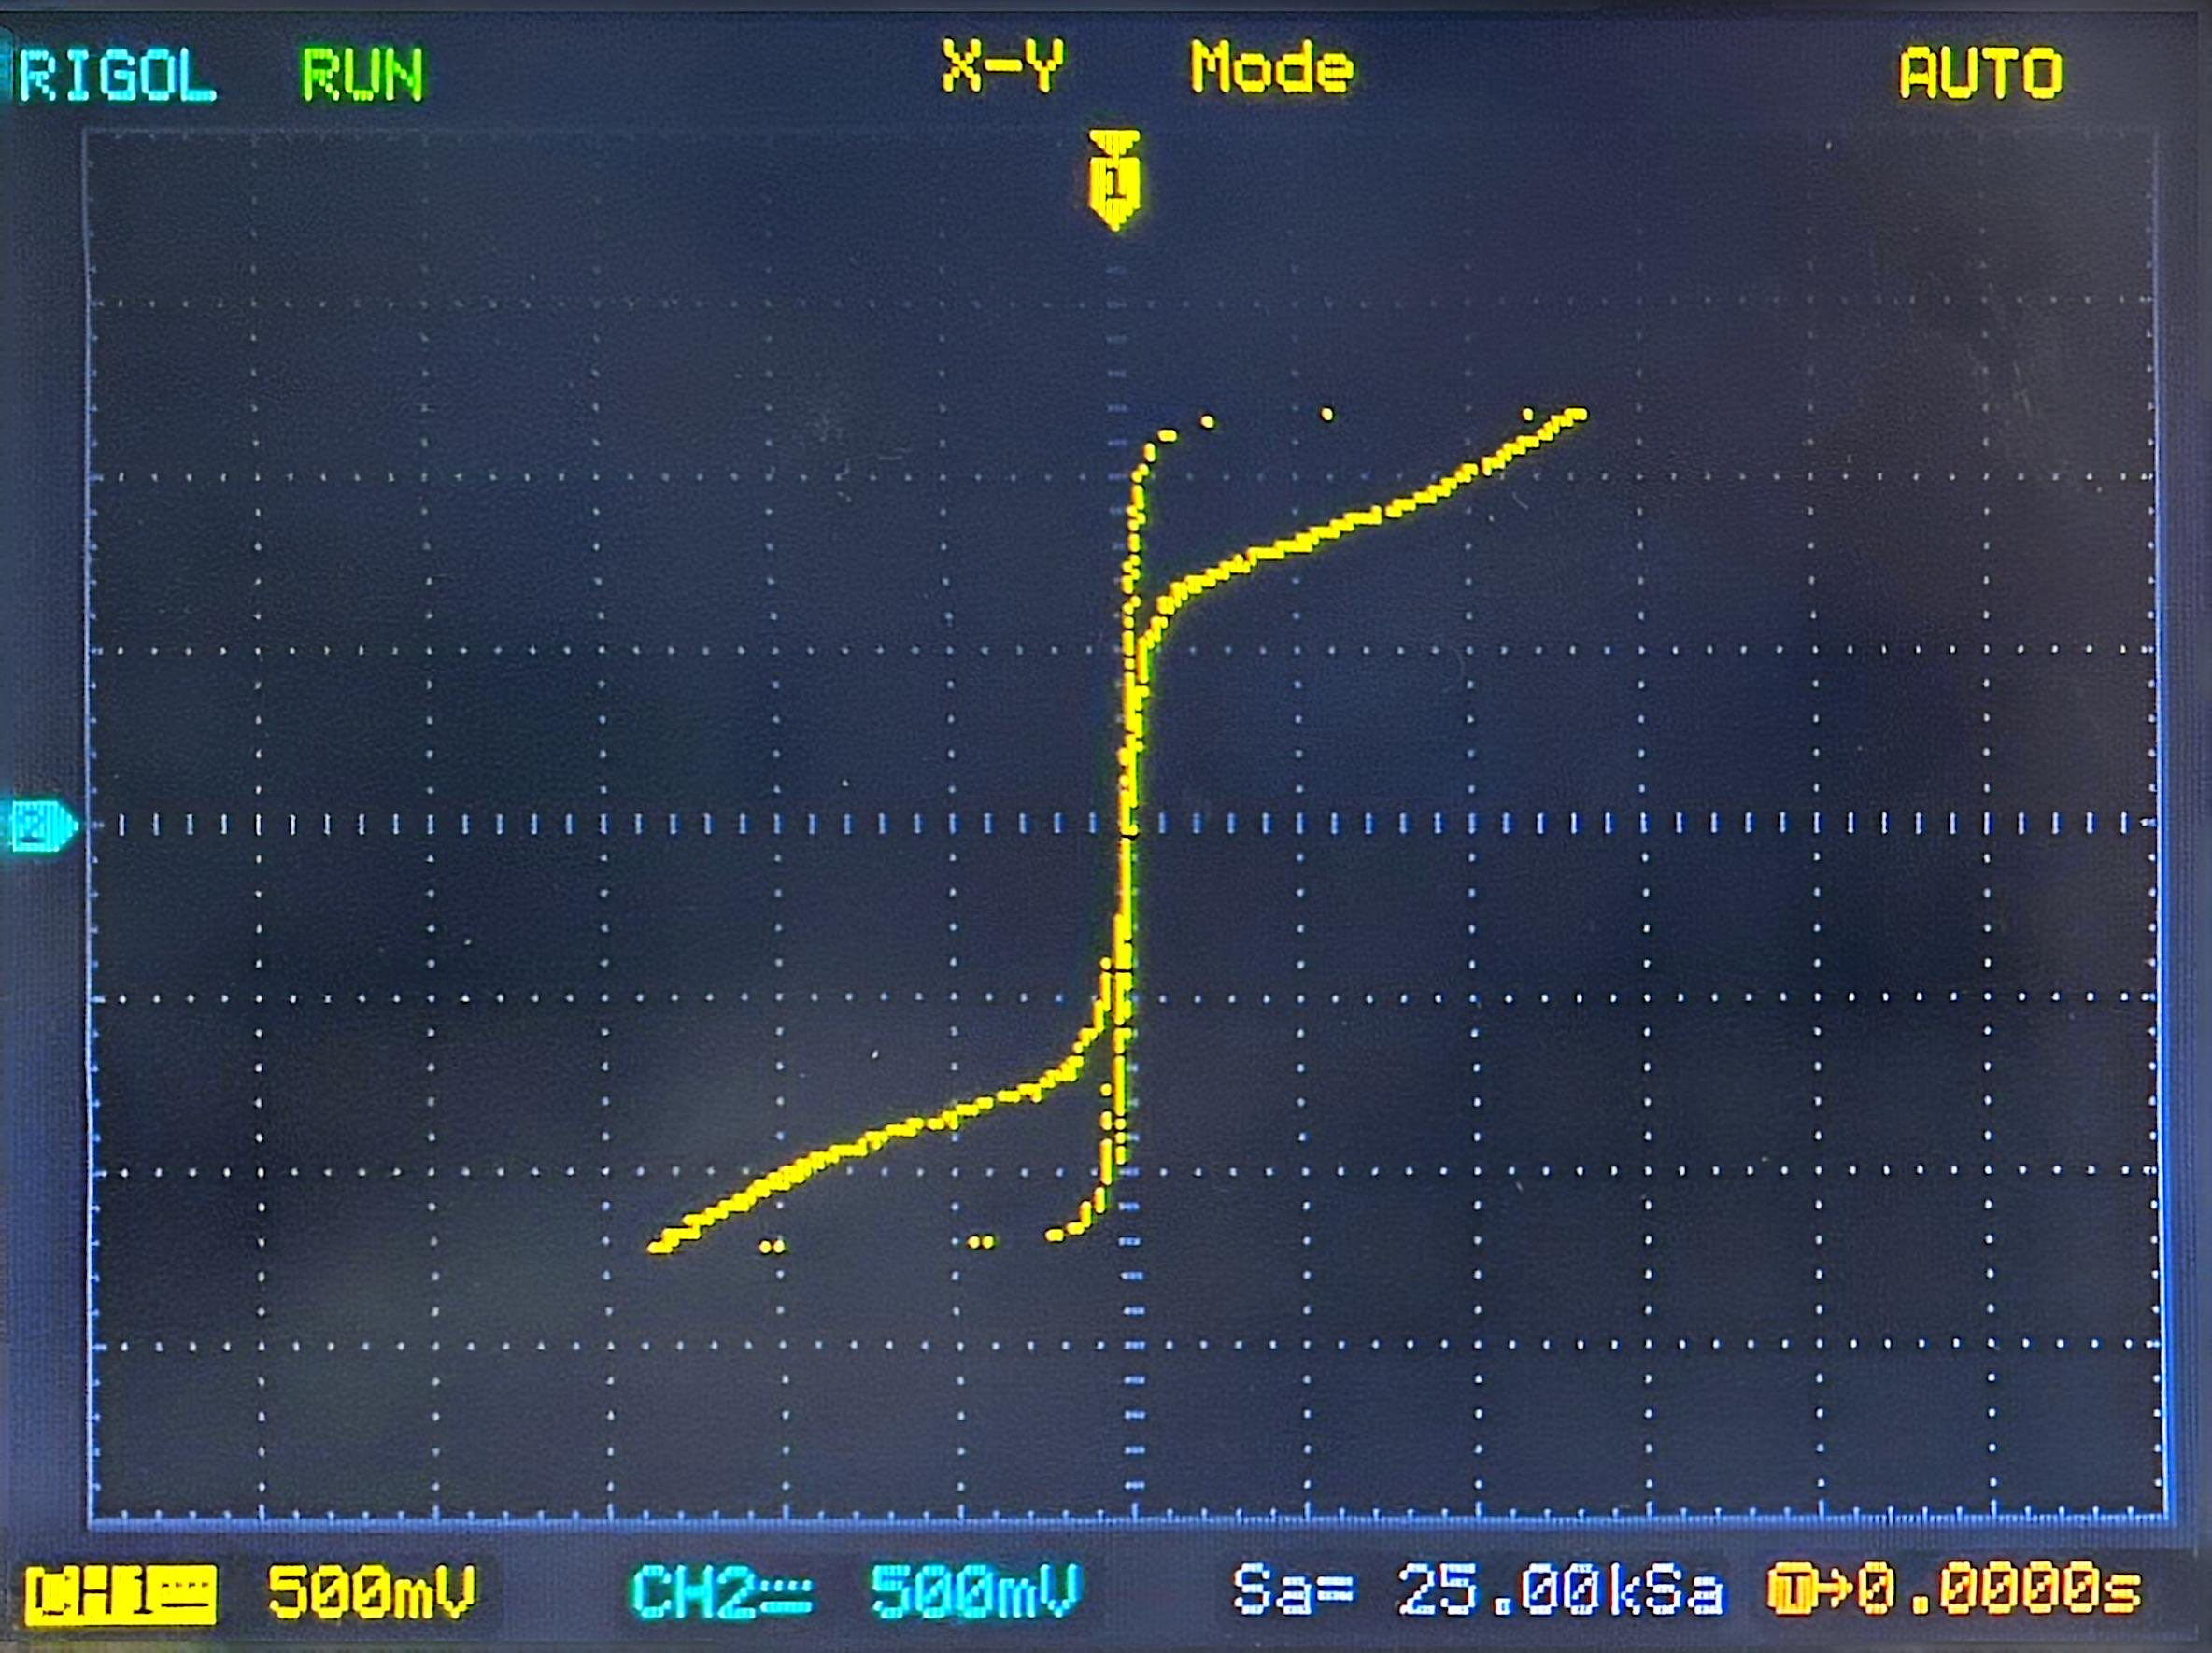
\includegraphics[height=120pt]{assets/1.1/(2)/IMG_1796.JPG}
    \caption{$R_2C = 0.01$ s}
\end{subfigure}\hfill
\begin{subfigure}[b]{0.33\columnwidth}\centering
    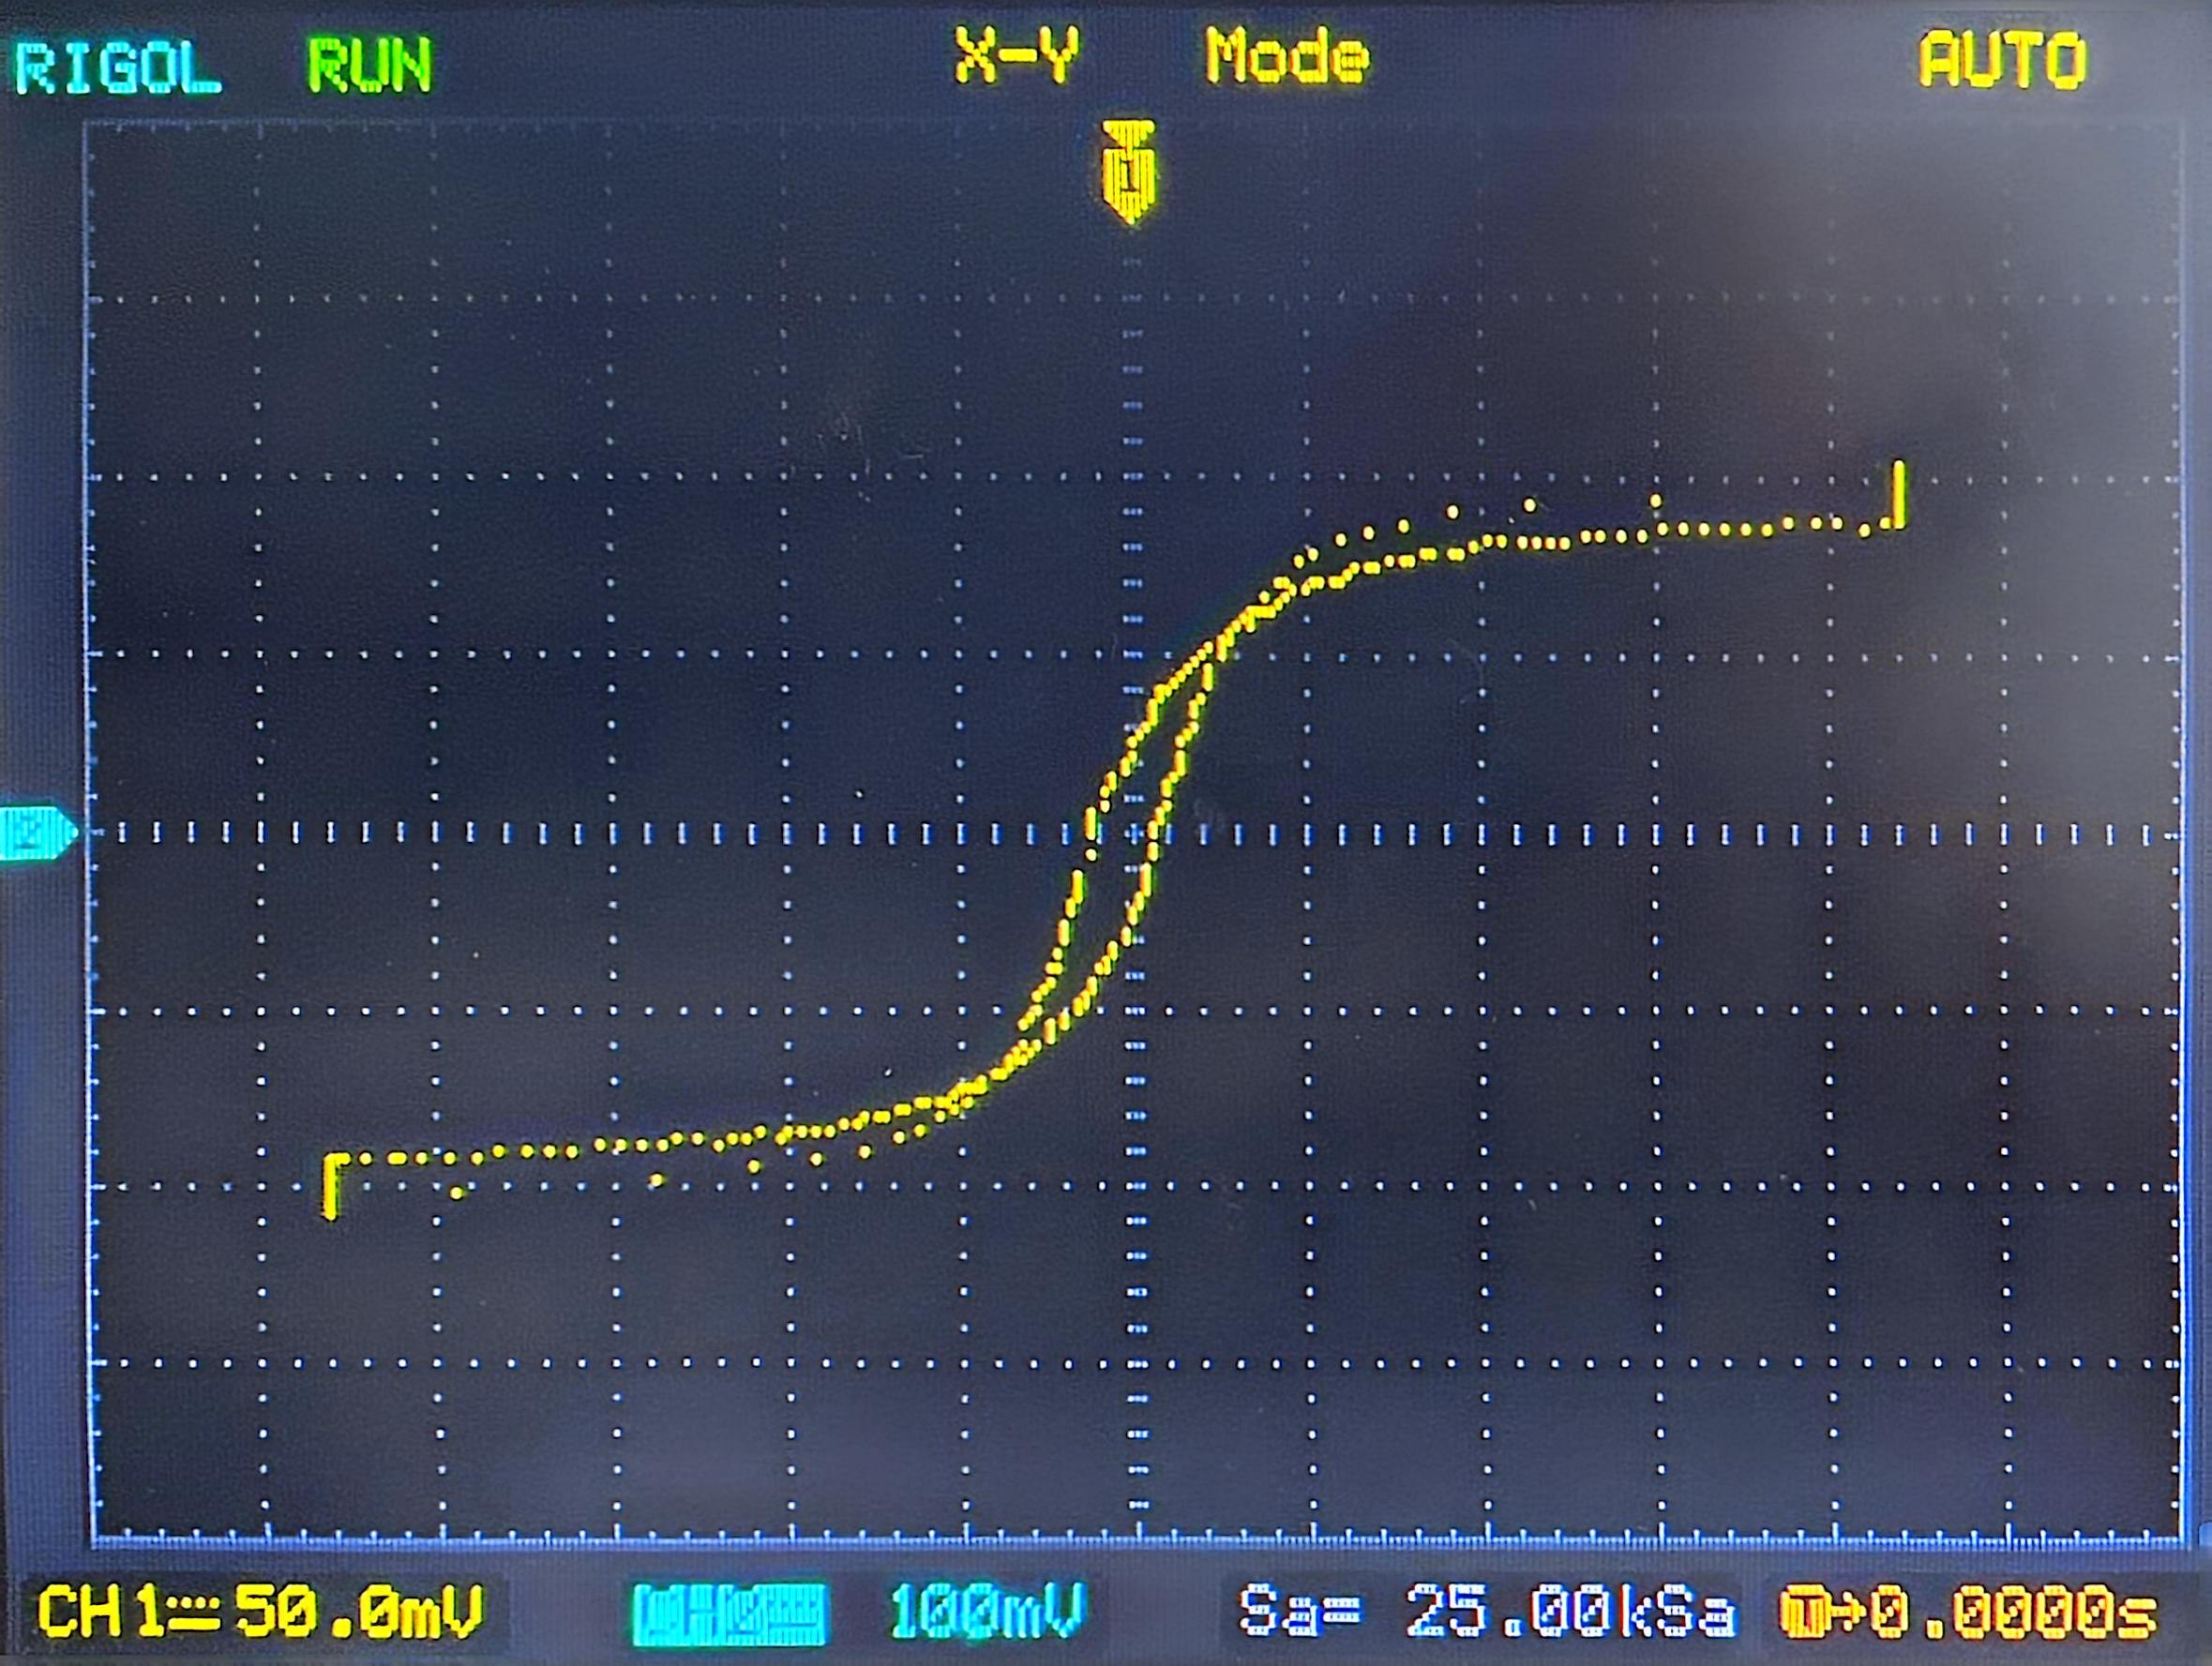
\includegraphics[height=120pt]{assets/1.1/(2)/IMG_1794.JPG}
    \caption{$R_2C = 0.05$ s}
\end{subfigure}
\begin{subfigure}[b]{0.33\columnwidth}\centering
    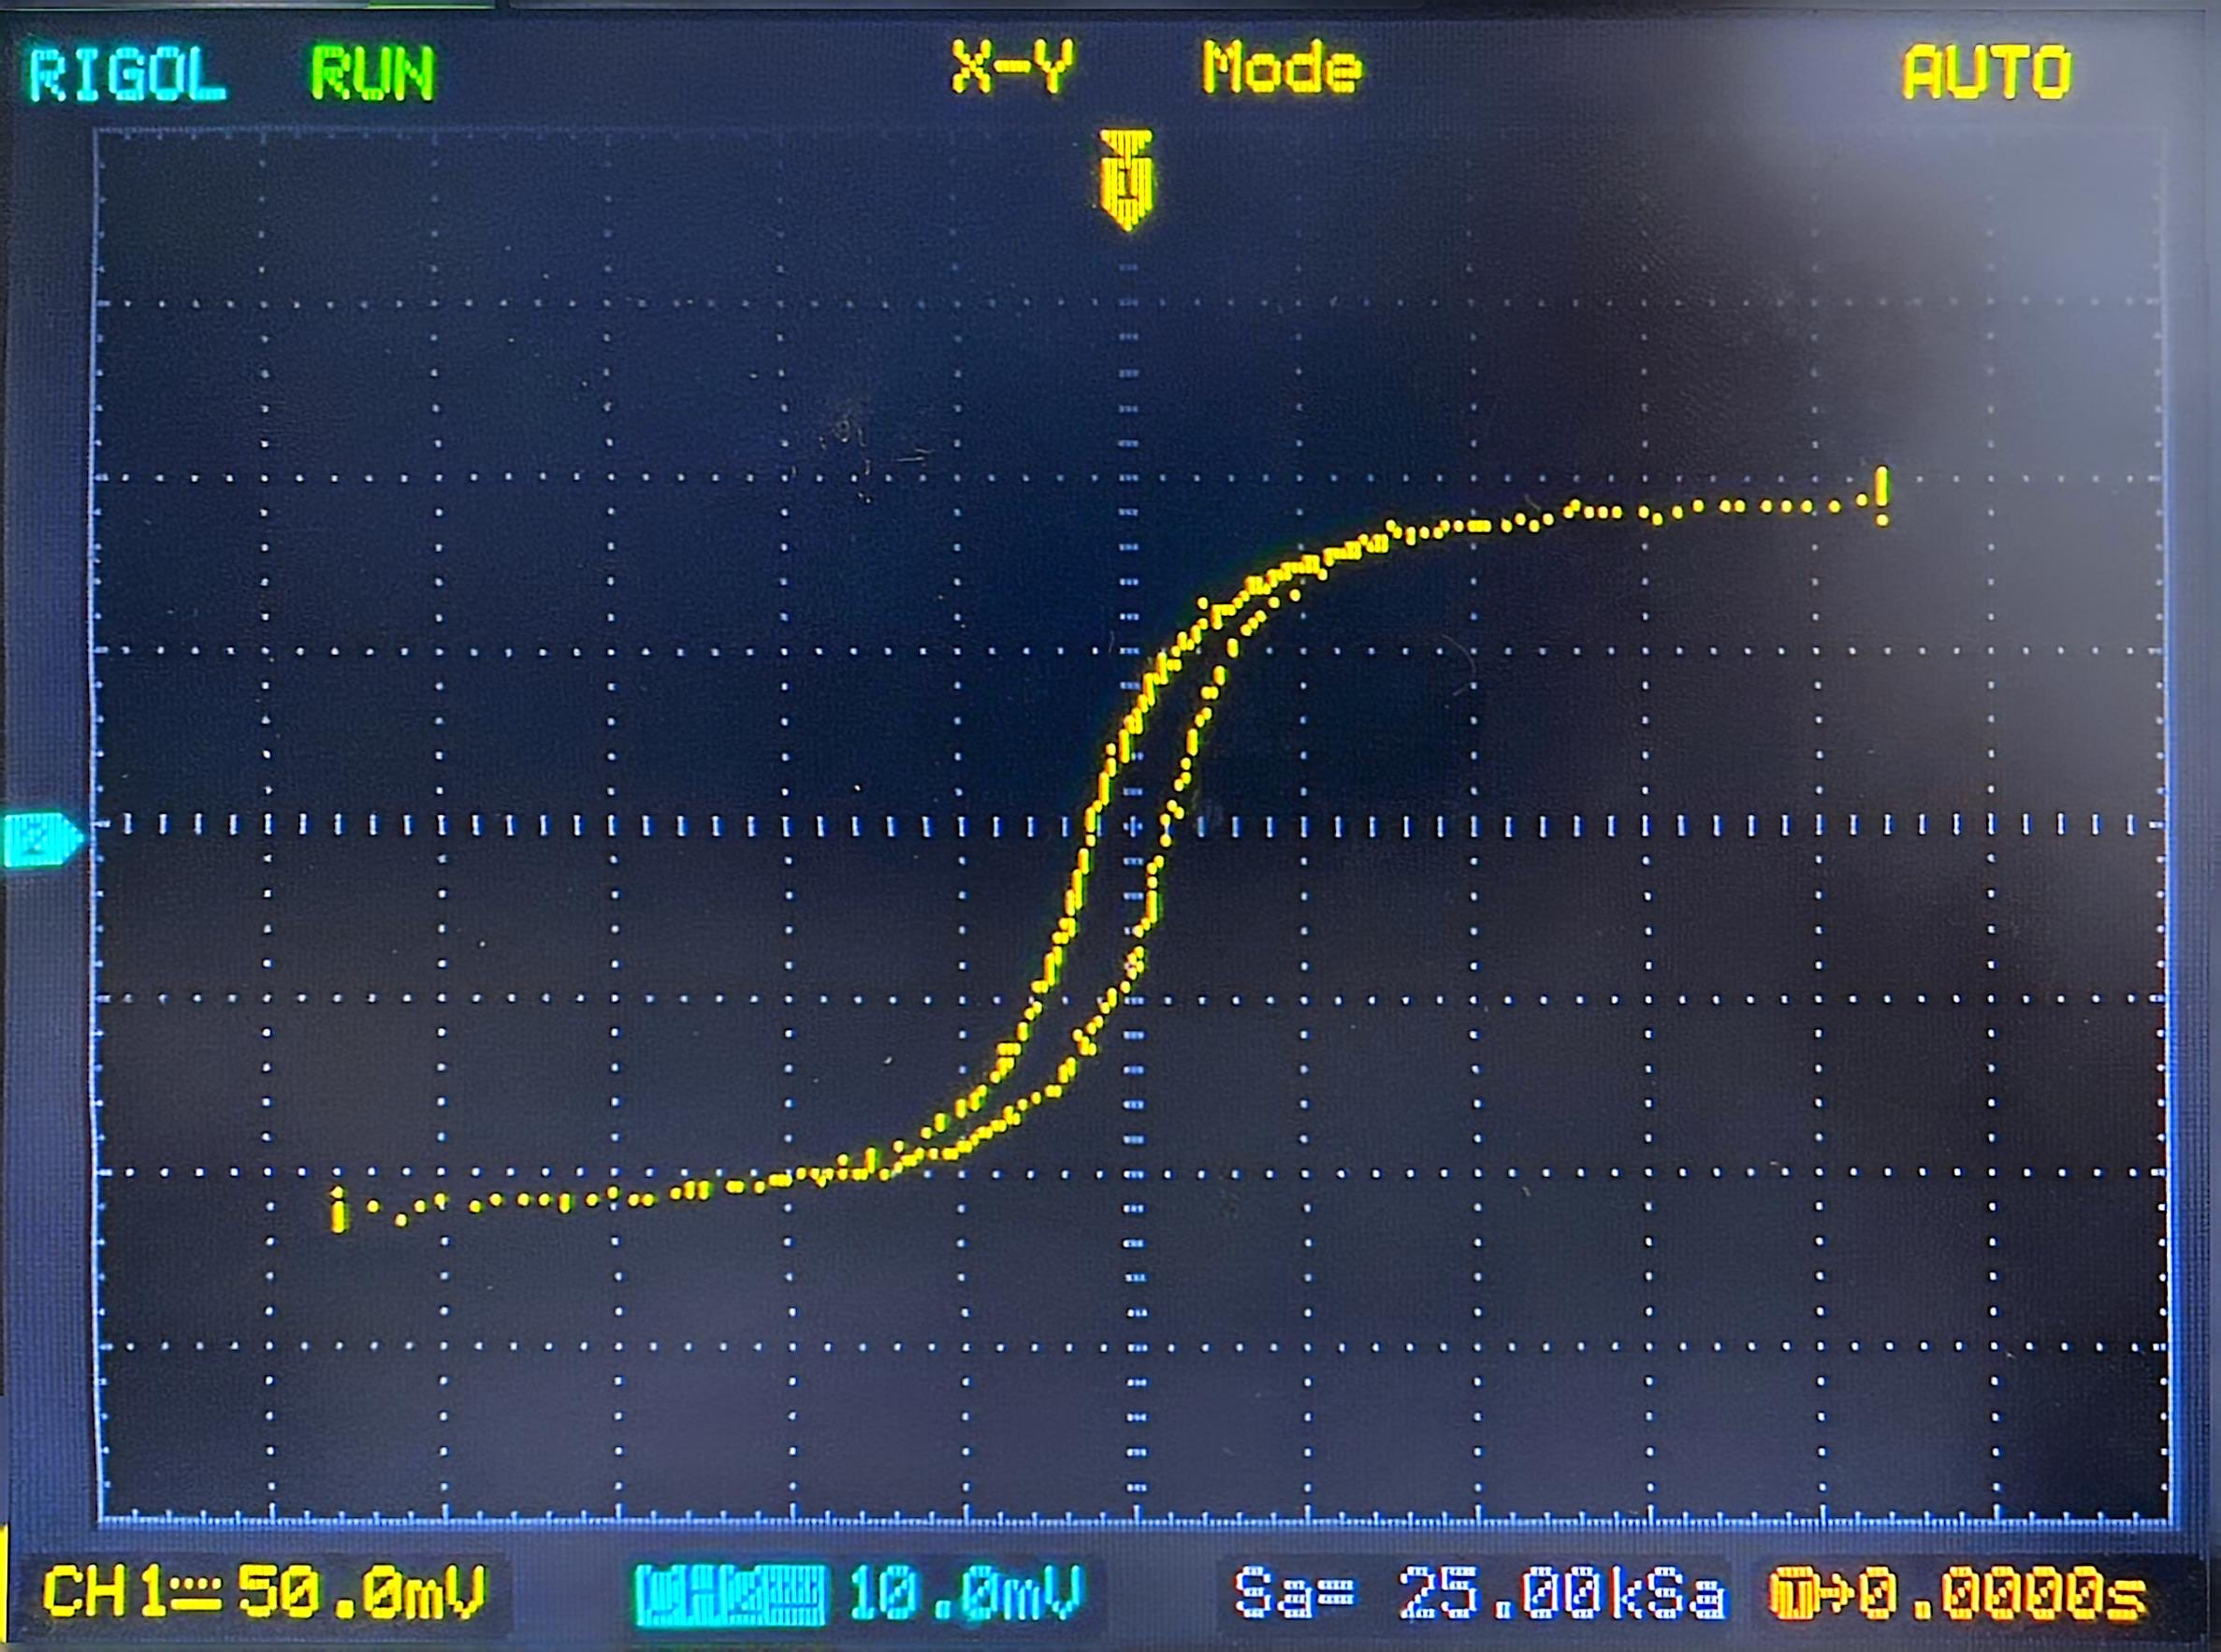
\includegraphics[height=120pt]{assets/1.1/(2)/IMG_1795.JPG}
    \caption{$R_2C = 0.5$ s}
\end{subfigure}
\caption{不同积分常量下的李萨如图形}
\end{figure}

\noindent Q1. 为什么积分常量会影响 $u_{R_1}-u_c$ 李萨如图形的形状?\par
实验原理中,公式${u_C} = \frac{Q}{C} = \frac{1}{C}\int {{i_2}dt}  = \frac{1}{{C{R_2}}}\int {{u_{{R_2}}}dt}  \approx \frac{1}{{C{R_2}}}\int {{u_2}dt}$
的推导最后用的是约等于,而约等于
的条件是积分常数$R_2 C \gg T$,本实验频率 $f=100Hz$,即 $T=0.01s$,因此,在积分常数为 $0.5$ s 时,此
条件基本上满足,而变为 $0.05$ s 与$ 0.5$ s时,该条件不再满足,因此会改变李萨如图形的形状。

\noindent Q2. 积分常量是否会影响真实的$ B − H $磁滞回线的形状?\par
$u_c$的改变会影响$u_x$和$u_y$的比例,但$u_x$与$u_y$只影响到示波器上显示的图像,而真实的 $B − H $磁
滞回线的形状并不会因为示波器的显示而改变,故积分常量本质上对真实的磁滞回线并无影响。

\subsubsection{实验二:测量样品 1(铁氧体)的动态磁化曲线}
本小节仍使用样品 1 (铁氧体),各参数值没有变化,与上一节完全相同,进而得到换算公式:
\begin{equation}\label{1.2换算公式}
\begin{matrix}\displaystyle
H_m = \frac{N_1}{l_{1, 1}R_1}\cdot \frac{\Delta u_{R_1}}{2} = 288.4615\ \Delta u_{R_1},\quad 
B_m = \frac{R_2 C}{N_2 S_1}\cdot \frac{\Delta u_C}{2} = 13.4409 \ \Delta u_C \vspace*{2mm}
\\ \displaystyle
\mu_m = \frac{B_m}{\mu_0H_m} =  7.9577 \times 10^{5} \cdot \frac{B_m}{H_m},\quad \mu_i = \lim_{H_m\to 0} \mu_m
\end{matrix}
\end{equation}
我们共测得 20 个数据点,原始电压测量结果见表 \ref{1.2电压},换算结果见表 \ref{1.2换算后}。

对磁化曲线,我们仍采用实验一中的函数 $y = f(x) = a \arctan (b x + c) + d$ 进行拟合,对于振幅磁导率 $\mu_m$,我们采用下面的拟合函数:
\begin{equation}
    y = f(x) = ae^{bx} + ce^{dx} + e
\end{equation}
其中 $a, b, c, d, e$ 为待定常数,且 $b,\ d < 0$。拟合优度如图 \ref{1.2拟合优度} 所示。依据原始数据和拟合结果,作出磁化曲线 $H_m$-$B_m$ 和振幅磁导率曲线 $\mu_m$-$H_m$,如图 \ref{1.2图} 所示\footnote{Matlab 源码见附录 \ref{1.2源码}}。

在 $\mu_m$ 的拟合结果,令自变量 $H_m = 0$,即可得到起始磁导率 $\mu_i$ :
\begin{equation}
\mu_i = \lim_{H_m\to 0} \mu_m = 10827.9292
\end{equation}

\newpage
\begin{center}
\noindent\begin{minipage}{0.25\columnwidth}
\begin{table}[H]\centering
        %\renewcommand{\arraystretch}{1.5} % 调整行间距为 1.5 倍
        %\setlength{\tabcolsep}{1.5mm} % 调整列间距
        \caption{原始电压数据点}
        \label{1.2电压}
    \begin{tabular}{cc}\toprule
$\Delta u_{R_1}$ (mV) & $\Delta u_{C}$ (mV) \\
\midrule
5.76	& 1.92 \\
7.00	& 2.48 \\
7.68	& 2.64 \\
10.2	& 3.60 \\
12.9	& 4.72 \\
15.9	& 5.92 \\
17.80	& 6.96 \\
24.8	& 9.84 \\
31.6	& 13.0 \\
42.4	& 17.2 \\
54.4	& 21.2 \\
61.6	& 23.2 \\
68.0	& 25.2 \\
74.4	& 26.4 \\
85.6	& 28.8 \\
93.6	& 30.4 \\
110	    & 32.4 \\
137	    & 34.4 \\
158	    & 36.0 \\
1070	& 42.4 \\
\bottomrule
    \end{tabular}
\end{table}
\end{minipage}\begin{minipage}{0.4\columnwidth}
\begin{table}[H]\centering
    %\renewcommand{\arraystretch}{1.5} % 调整行间距为 1.5 倍
    %\setlength{\tabcolsep}{1.5mm} % 调整列间距
    \caption{换算后的磁化曲线与振幅磁导率}
    \label{1.2换算后}
    \begin{tabular}{ccc}\toprule
$H_m$ $\mathrm{(A\cdot m^{-1})}$ & $B_m$ (T) & $\mu_m$ (1) \\
\midrule
1.662	& 0.026 & 12359.70 \\
2.019	& 0.033 & 13136.60 \\
2.215	& 0.035 & 12745.94 \\
2.942	& 0.048 & 13086.74 \\
3.721	& 0.063 & 13566.93 \\
4.587	& 0.080 & 13805.55 \\
5.135	& 0.094 & 14498.35 \\
7.154	& 0.132 & 14712.03 \\
9.115	& 0.175 & 15254.06 \\
12.231  & 0.231 & 15041.53 \\
15.692  & 0.285 & 14449.95 \\
17.769  & 0.312 & 13964.86 \\
19.615  & 0.339 & 13741.08 \\
21.462  & 0.355 & 13157.10 \\
24.692  & 0.387 & 12475.21 \\
27.000  & 0.409 & 12042.79 \\
31.731  & 0.435 & 10921.48 \\
39.519  & 0.462 & 9310.37 \\
45.577  & 0.484 & 8448.40 \\
308.654 & 0.570 & 1469.30 \\
\bottomrule
\end{tabular}
\end{table}
\end{minipage}
\begin{minipage}{0.28\columnwidth}
\begin{figure}[H]\centering
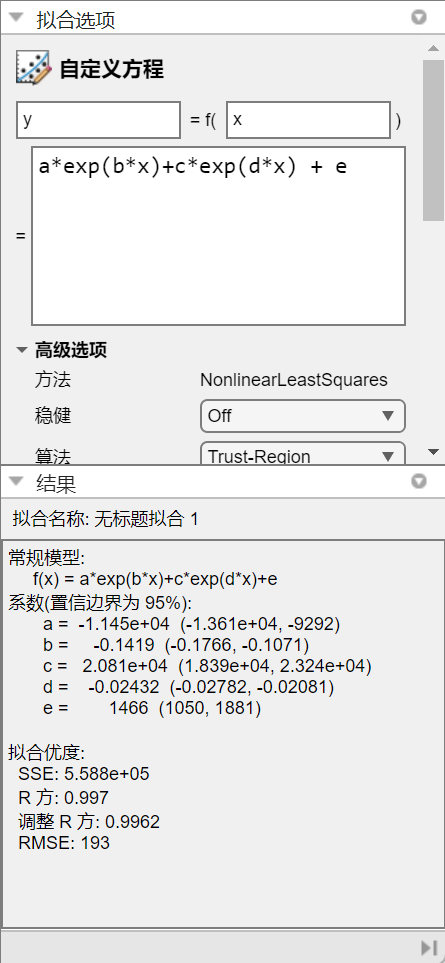
\includegraphics[width=\columnwidth]{assets/1.2/fd7e40fc533d62dd25043cc43de0afe8.png}
\caption{$\mu_m$ 拟合优度}\label{1.2拟合优度}
\end{figure}
\end{minipage}
\end{center}

\begin{figure}[H]\centering
\begin{subfigure}[b]{0.5\columnwidth}\centering
    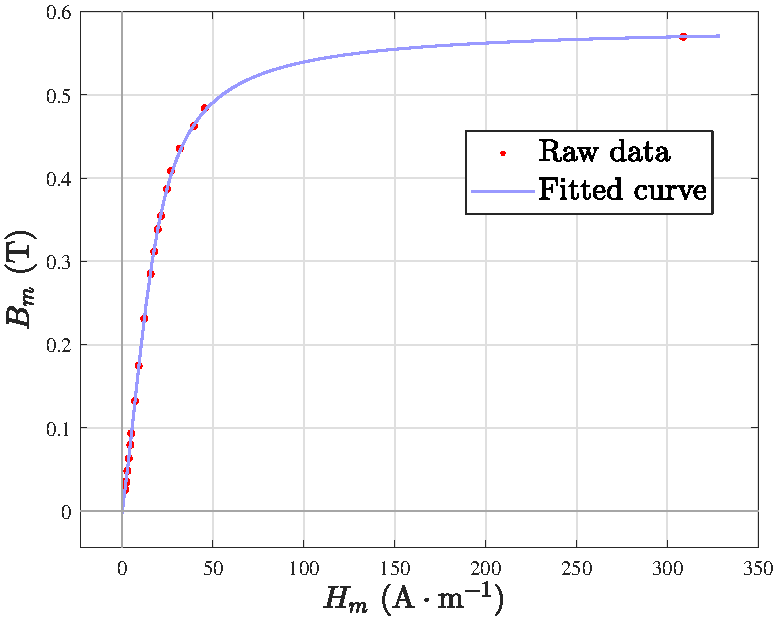
\includegraphics[height=185pt]{assets/1.2/2024-10-28_23-27-43.pdf}
    \caption{磁化曲线 $H_m$-$B_m$}
\end{subfigure}\hfill
\begin{subfigure}[b]{0.5\columnwidth}\centering
    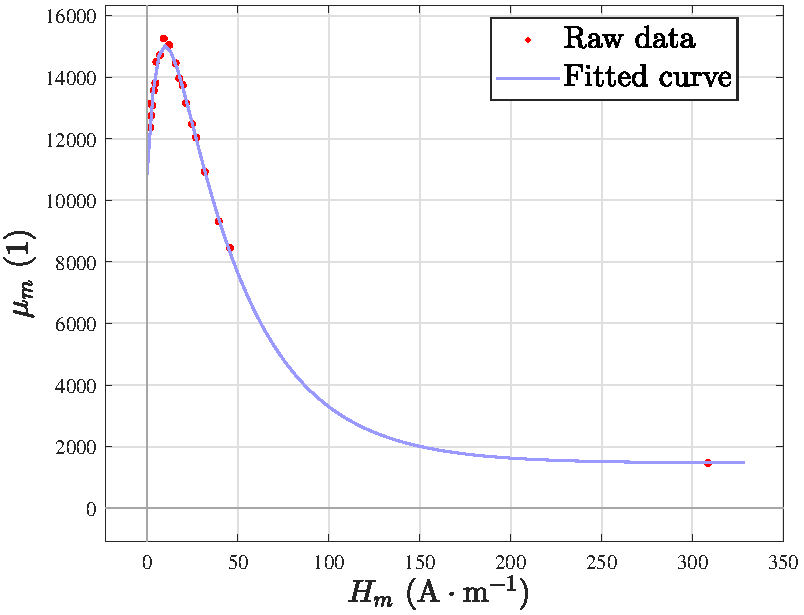
\includegraphics[height=185pt]{assets/1.2/2024-10-28_23-28-14.pdf}
    \caption{振幅磁导率曲线 $\mu_m$-$H_m$}
\end{subfigure}
\caption{磁化曲线和振幅磁导率曲线}\label{1.2图}
\end{figure}


\subsubsection{实验三:观察不同频率下样品 2(硅钢)的动态磁滞回线}\label{不同频率硅钢}
本小节使用样品 2,因此长度和面积参数应改为 $l_{1,2}$ 和 $S_2$,其它参数不变,于是有换算公式 (\ref{1.3换算公式})。

\begin{equation}\label{1.3换算公式}
    H = \frac{N_1}{l_{1, 2}R_1}\cdot u_{R_1} = 1000.00 \cdot u_{R_1},\quad 
    B = \frac{R_2 C}{N_2 S_2}\cdot u_C = 27.7778  u_C
\end{equation}

实验时的照片如图 \ref{1.3图} 所示,最终结果如表 \ref{1.3表} 所示。
\begin{figure}[H]\centering
\begin{subfigure}[b]{0.33\columnwidth}\centering
    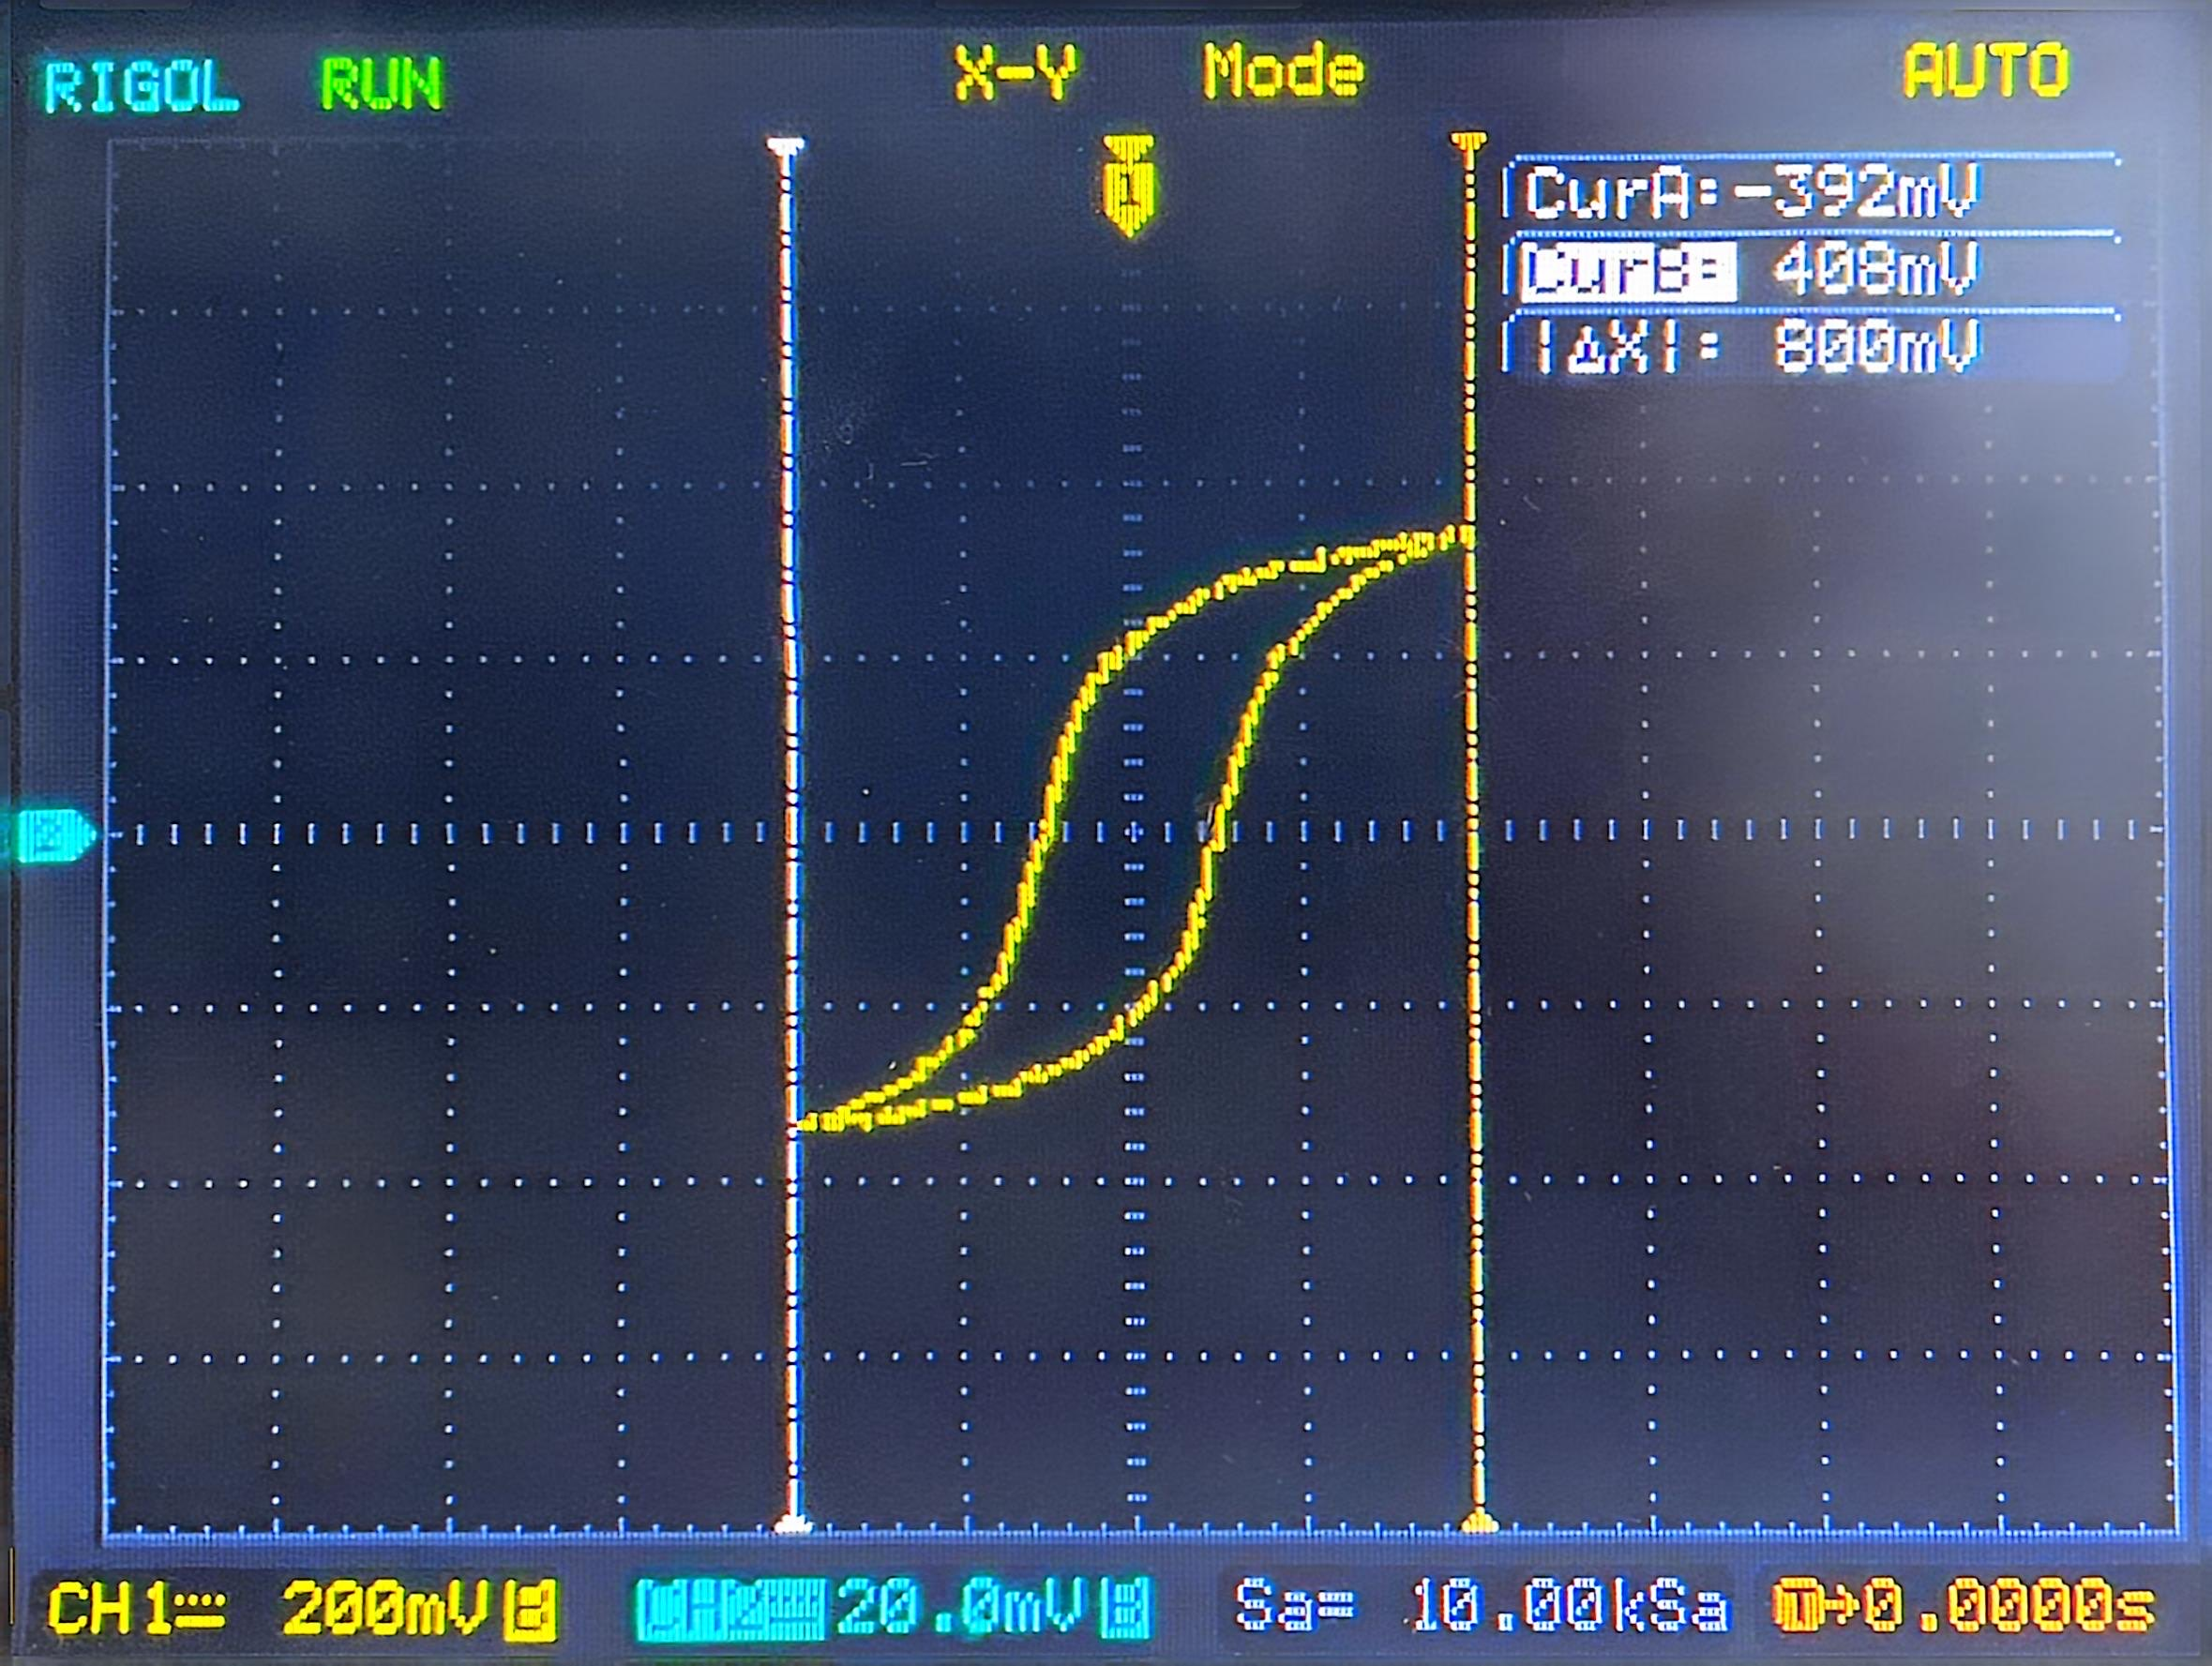
\includegraphics[height=120pt]{assets/1.3/IMG_1793.JPG}
    \caption{$f = 20$ Hz}
\end{subfigure}\hfill
\begin{subfigure}[b]{0.33\columnwidth}\centering
    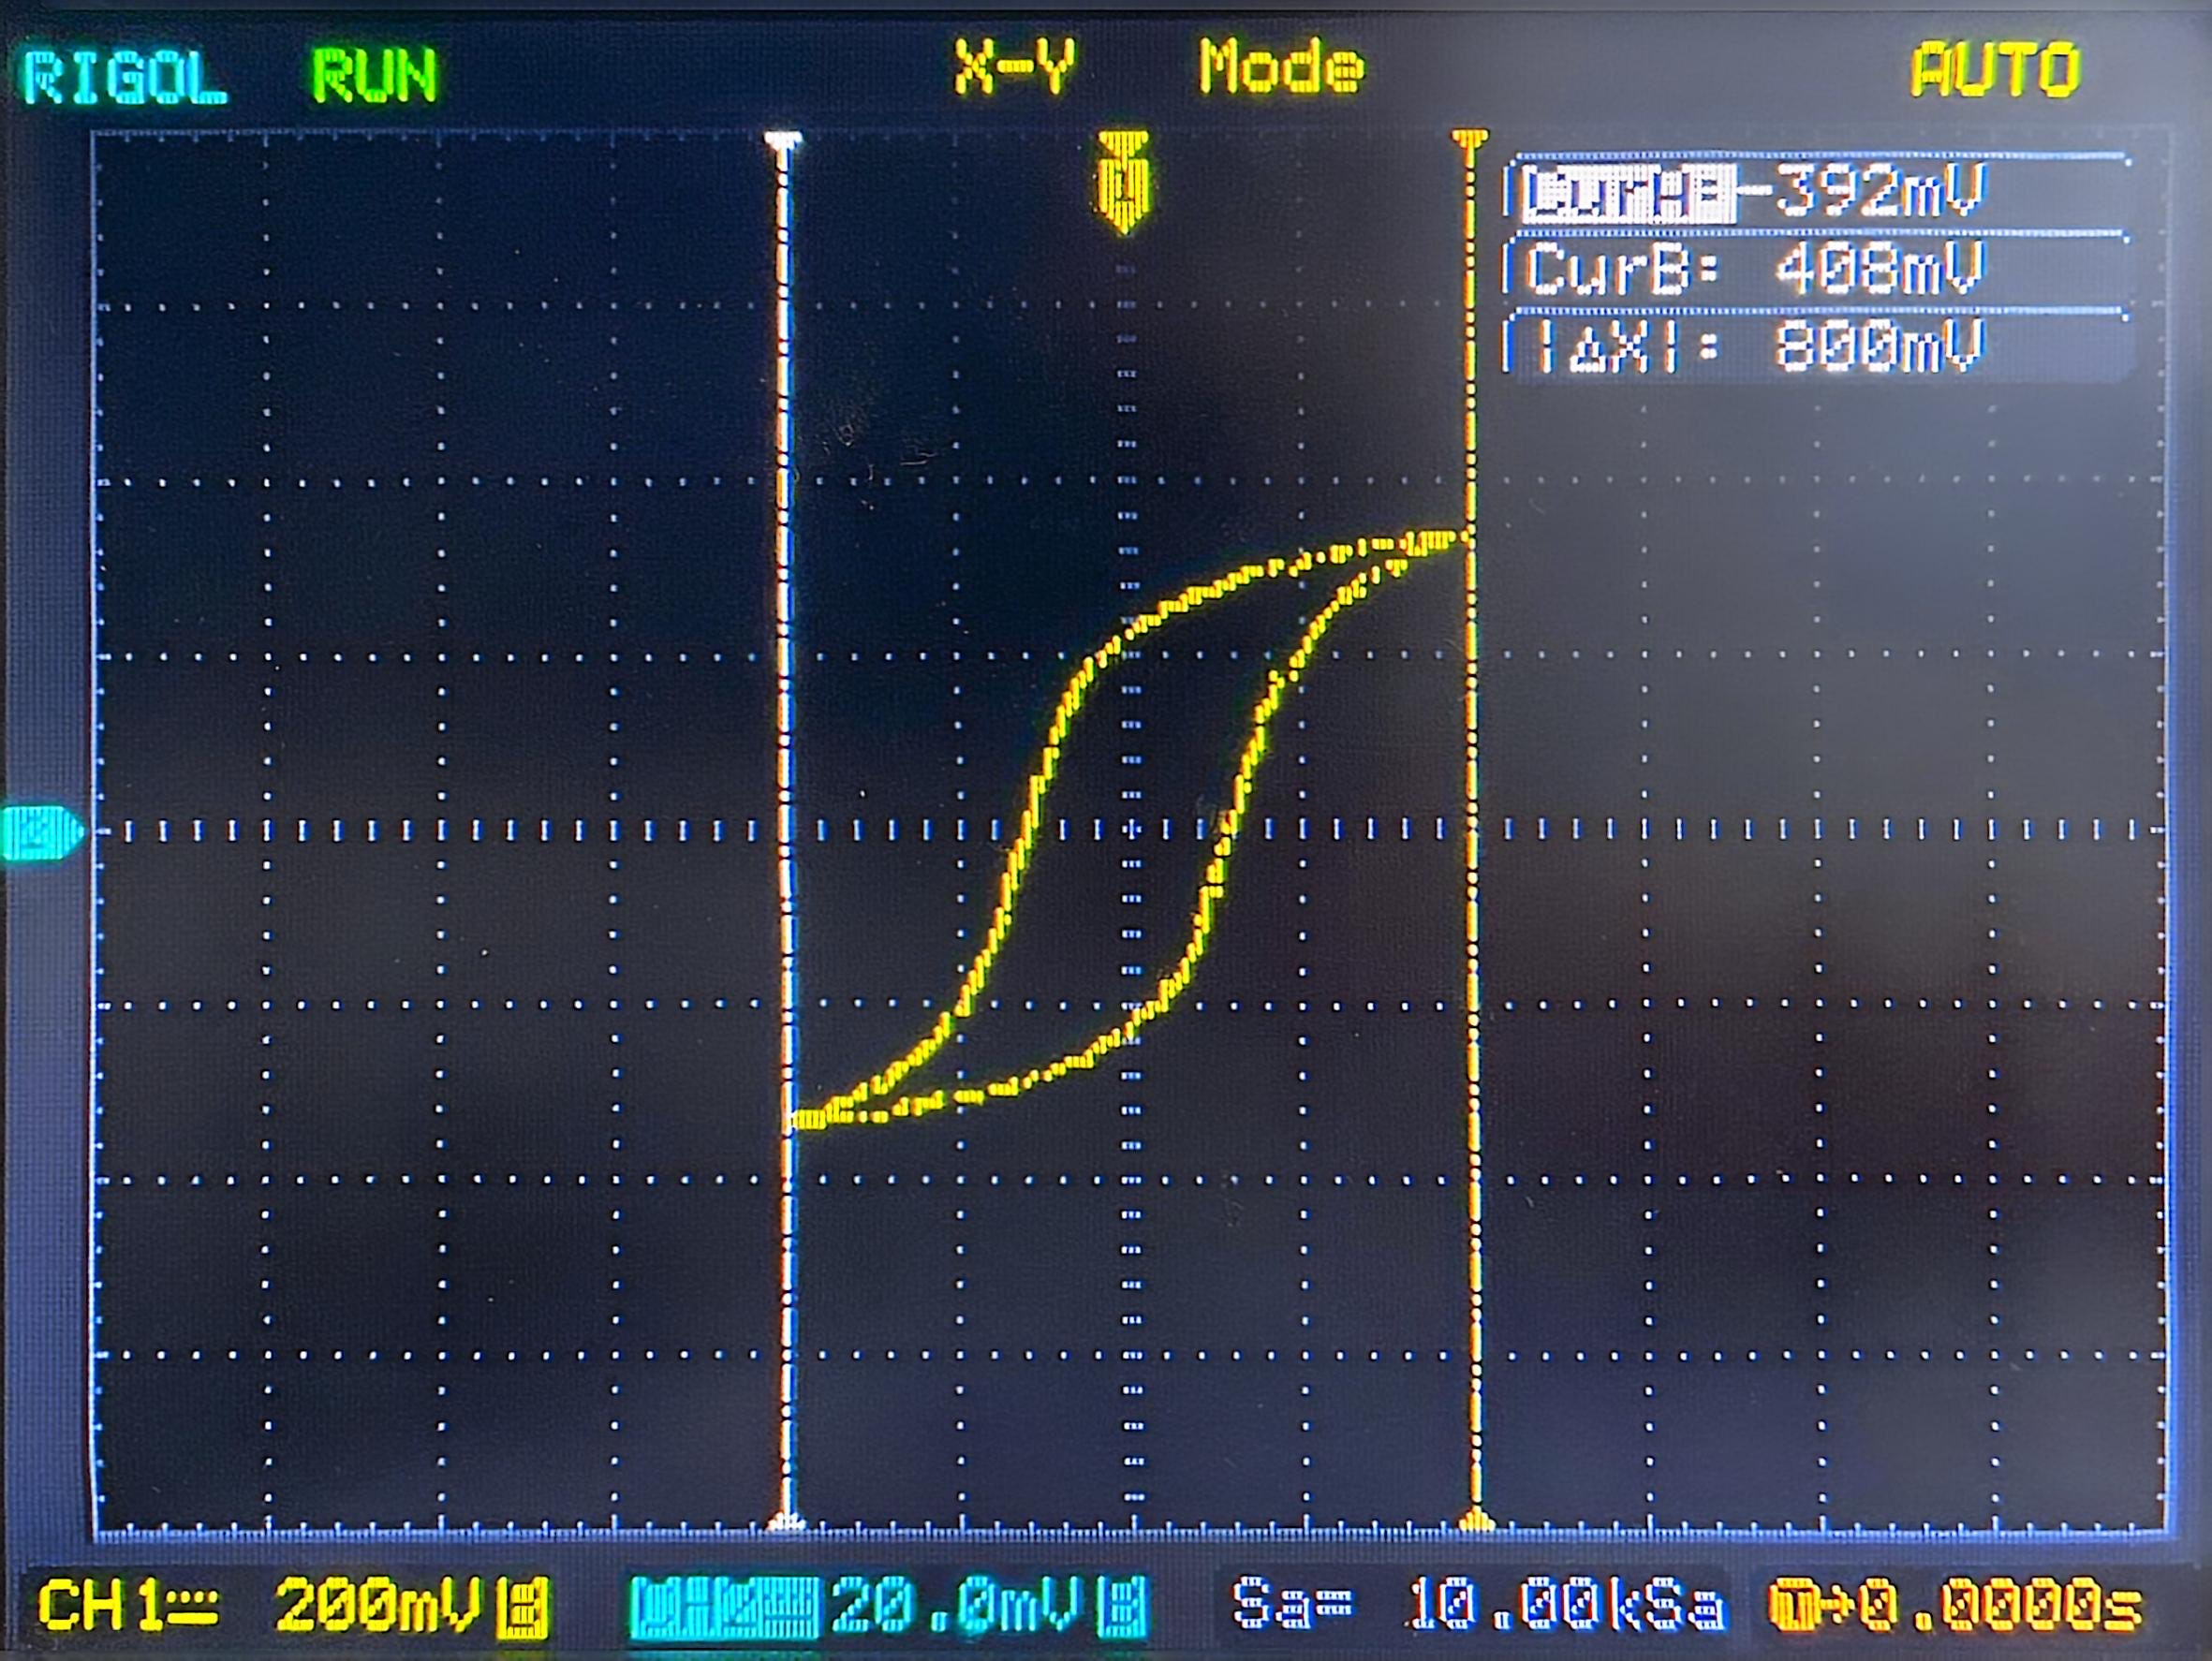
\includegraphics[height=120pt]{assets/1.3/IMG_1792.JPG}
    \caption{$f = 40$ Hz}
\end{subfigure}
\begin{subfigure}[b]{0.33\columnwidth}\centering
    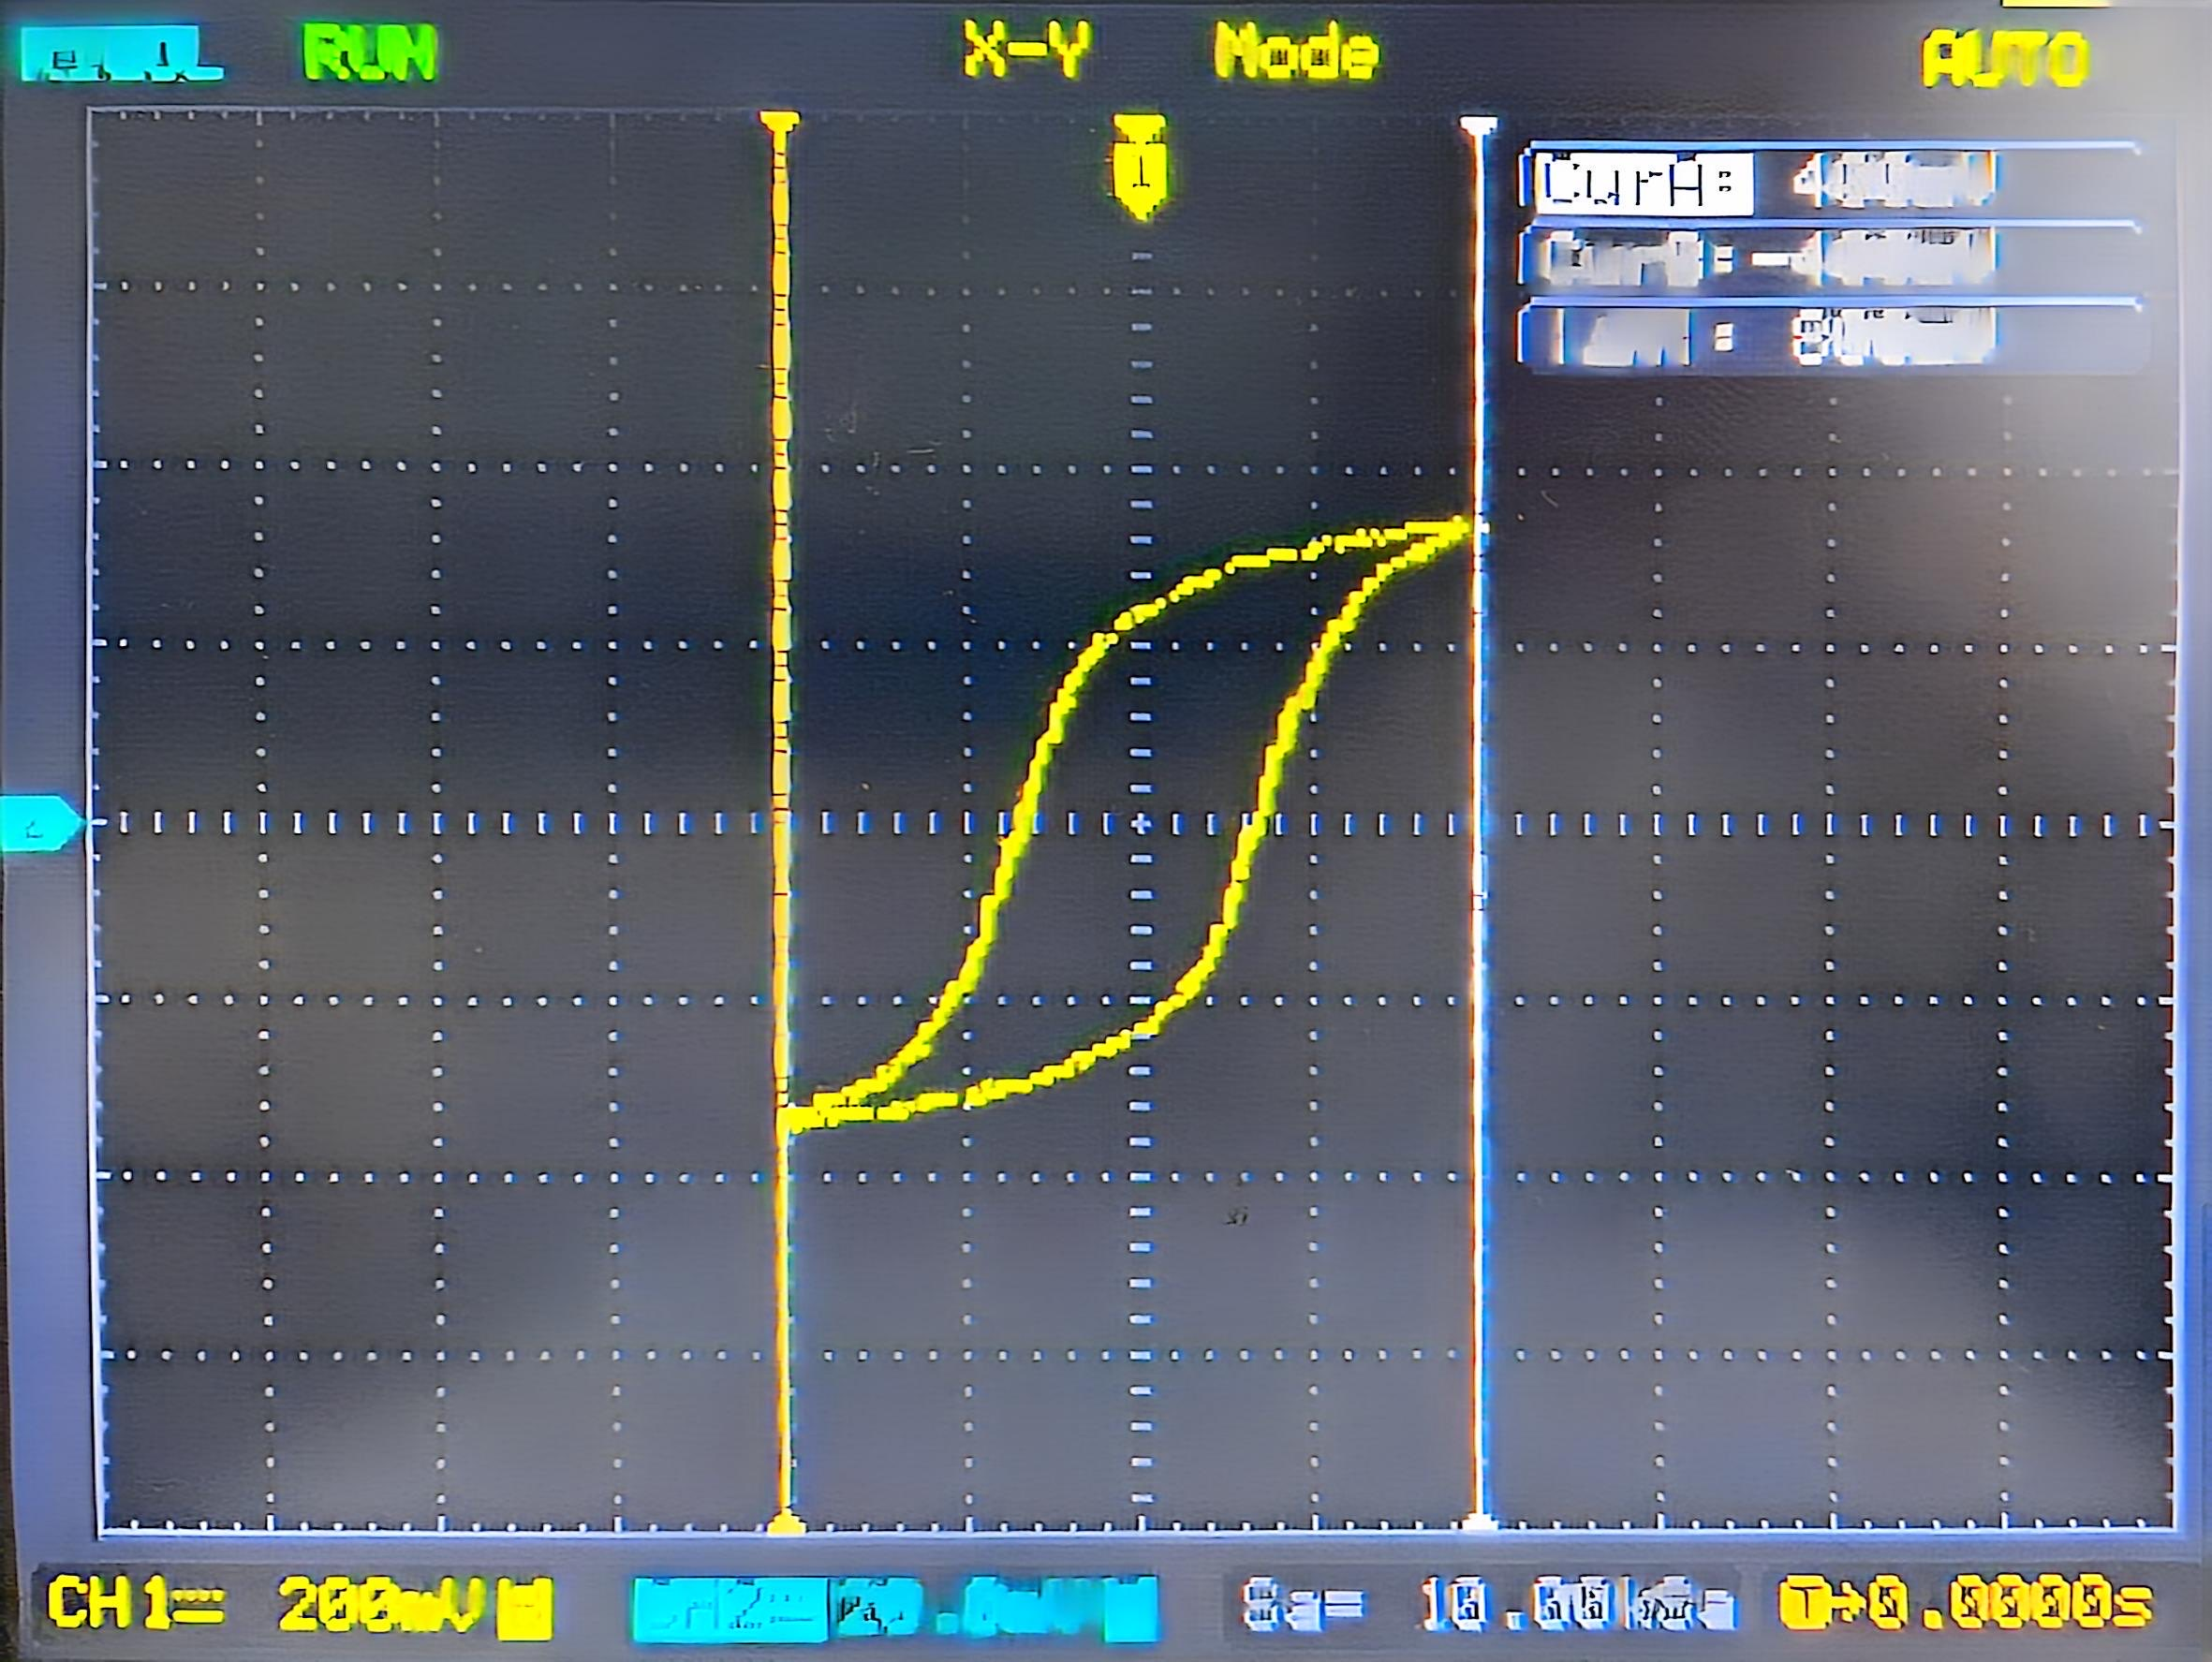
\includegraphics[height=120pt]{assets/1.3/IMG_1791.JPG}
    \caption{$f = 60$ Hz}
\end{subfigure}
\caption{不同频率下样品 2(硅钢)的动态磁滞回线}\label{1.3图}
\end{figure}

\vspace*{-5mm}
\begin{center}
    \noindent\begin{minipage}{0.49\columnwidth}
    \begin{table}[H]\centering
        %\renewcommand{\arraystretch}{1.5} % 调整行间距为 1.5 倍
        %\setlength{\tabcolsep}{1.5mm} % 调整列间距
        \caption{原始电压数据}
    \begin{tabular}{cccccccccc}\toprule
        $f$ (Hz) & 20 & 40 & 60  \\
        \midrule
        $B_m$ 对应的 $u_{C}$ (mV) & 33.6 & 33.6 & 33.6 \\
        $B_r$ 对应的 $u_{C}$(mV) & 20.8 & 23.2 & 24.0 \\
        $H_c$ 对应的 $u_{R_1}$(mV) & 112  & 128  & 144 \\
        \bottomrule
    \end{tabular}
    \end{table}
\end{minipage}\begin{minipage}{0.49\columnwidth}
    \begin{table}[H]\centering
        %\renewcommand{\arraystretch}{1.5} % 调整行间距为 1.5 倍
        %\setlength{\tabcolsep}{1.5mm} % 调整列间距
        \caption{不同频率时的 $B_r$ 和 $H_c$}
        \begin{tabular}{cccccccccc}\toprule
            $f$ (Hz) & 20 & 40 & 60  \\
            \midrule
            $B_m$ (T) & 0.9333 & 0.9333 & 0.9333 \\
            $B_r$ (T) & 0.5778  & 0.6444 & 0.6667 \\
            $H_c$ $\mathrm{A\cdot m^{-1}}$ & 112  & 128  & 144 \\
            \bottomrule
        \end{tabular}
    \end{table}\label{1.3表}
\end{minipage}
\end{center}
由表可见,随着频率的增大,$B_m$ 基本不变化,而 $B_r$ 和 $H_c$ 均不断增大,磁滞回线所围成的面积(正比于磁滞损耗)也不断增大,与之前样品 1(铁氧体)的结论恰好相反。这些都和理论推导相符合。

\subsubsection{实验四:测量样品 1(铁氧体)在不同直流偏置磁场下的可逆磁导率}
本小节又换回样品 1,且参数 $R_2$ 和 $C$ 发生了变化,$R_1 = 2.0 \ \Omega$,$R_2 = 20.0 \kO$,$C = 2 \uF$,相应的换算公式变为公式 (\ref{1.4换算公式}),式中的 $H$ 是指当前的直流偏置磁场强度。
\begin{equation}\label{1.4换算公式}
\begin{matrix}\displaystyle
    H = \frac{N_3}{l_{1,1}}\cdot I = 1.1538 \times 10^3 \cdot I,\quad 
    \mu_R = \frac{1}{\mu_0}\cdot\frac{\Delta B}{\Delta H} = \frac{R_1R_2C l_{1,1}}{\mu_0N_1N_2S_1} \cdot \frac{\Delta u_{C}}{\Delta u_{R_1}} = 2.9663\times 10^{3} \cdot \frac{\Delta u_{C}}{\Delta u_{R_1}}
\end{matrix}
\end{equation}

采用函数 $y = f(x) = ae^{bx}$ 对 $\mu_R$ 进行拟合(自变量为偏置磁场 $H$),其中 $a, b$ 为待定常数,且 $b < 0$。拟合优度如图 \ref{1.4优度} 所示。作出可逆磁导率 $\mu_R$ 随偏置磁场 $H$ 的变化曲线,如图 \ref{1.4图} (a)\footnote{Matlab 源码见附录 \ref{1.4源码}} 所示。

\begin{figure}[H]\centering
    \begin{subfigure}[b]{0.5\columnwidth}\centering
        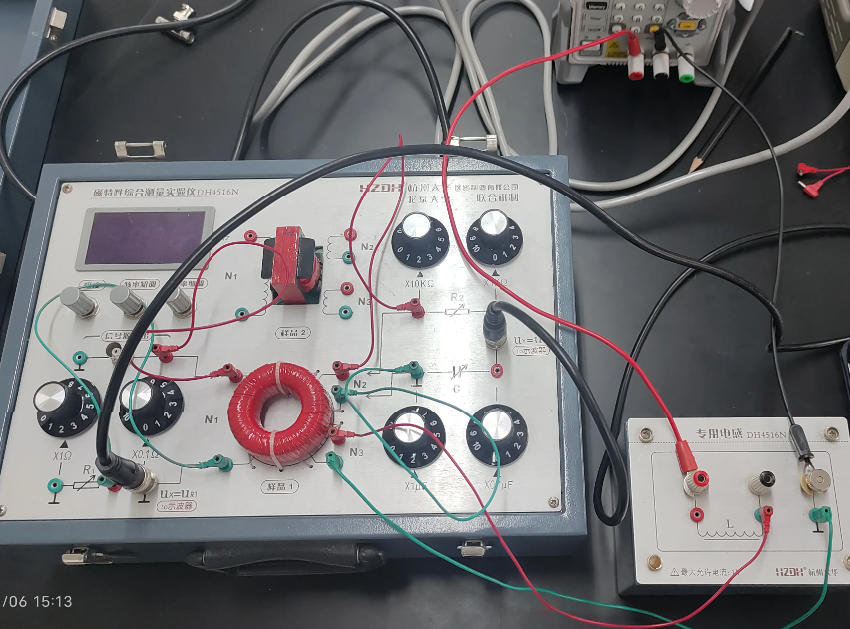
\includegraphics[height=165pt]{assets/1.4/image (9).png}
        \vspace*{3.5mm}
        \caption{直流偏置接线示意图}
    \end{subfigure}\hfill
\begin{subfigure}[b]{0.5\columnwidth}\centering
    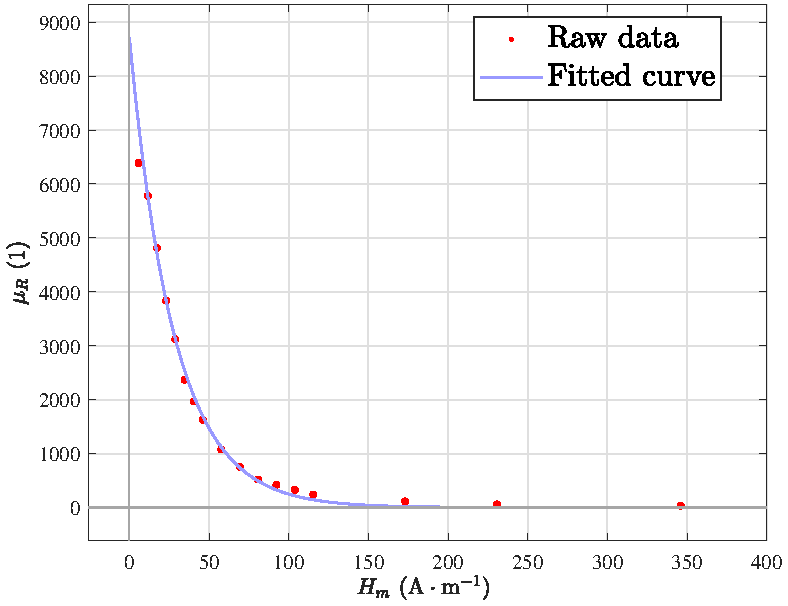
\includegraphics[height=180pt]{assets/1.4/2024-10-29_00-27-21.pdf}
    \caption{可逆磁导率 $\mu_R$ 随偏置磁场 $H$ 的变化曲线}
\end{subfigure}
\caption{实验装置与测量结果}\label{1.4图}
\end{figure}


\begin{center}
\noindent\begin{minipage}{0.35\columnwidth}
\begin{table}[H]\centering
        %\renewcommand{\arraystretch}{1.5} % 调整行间距为 1.5 倍
        %\setlength{\tabcolsep}{1.5mm} % 调整列间距
        \caption{原始电压数据点}
        \label{1.4电压}
    \begin{tabular}{ccc}\toprule
$I$ (A) & $\Delta u_{R_1}$ (mV) & $\Delta u_C$ (mV) \\
\midrule
0.005	& 2.60 & 5.60 \\
0.01	& 7.60 & 14.8 \\
0.015	& 7.40 & 12.0 \\
0.02	& 11.6 & 15.0 \\
0.025	& 11.6 & 12.2 \\
0.03	& 18.8 & 15.0 \\
0.035	& 18.4 & 12.2 \\
0.04	& 24.8 & 13.6 \\
0.05	& 20.4 & 7.40 \\
0.06	& 22.8 & 5.80 \\
0.07	& 24.0 & 4.20 \\
0.08	& 24.0 & 3.40 \\
0.09	& 23.6 & 2.60 \\
0.10	& 37.2 & 3.00 \\
0.15	& 36.8 & 1.40 \\
0.2	    & 124 & 2.40 \\
0.3	    & 124 & 1.40 \\
\bottomrule
    \end{tabular}
\end{table}
\end{minipage}\begin{minipage}{0.35\columnwidth}
\begin{table}[H]\centering
    %\renewcommand{\arraystretch}{1.5} % 调整行间距为 1.5 倍
    %\setlength{\tabcolsep}{1.5mm} % 调整列间距
    \caption{可逆磁导率随偏置磁场的变化}
    \label{1.4换算后}
    \begin{tabular}{ccc}\toprule
$H$ $\mathrm{(A\cdot m^{-1})}$ & $\mu_R$ (1) \\
\midrule
5.769	& 6389.016 \\
11.538	& 5776.535 \\
17.308	& 4810.263 \\
23.077	& 3835.770 \\
28.846	& 3119.759 \\
34.615	& 2366.752 \\
40.385	& 1966.805 \\
46.154	& 1626.696 \\
57.692	& 1076.021 \\
69.231	& 754.592  \\
80.769	& 519.108  \\
92.308	& 420.230  \\
103.846	& 326.799  \\
115.385	& 239.220  \\
173.077	& 112.849  \\
230.769	& 57.413   \\
346.154	& 33.491   \\
\bottomrule
\end{tabular}
\end{table}
\end{minipage}\begin{minipage}{0.25\columnwidth}
\begin{figure}[H]\centering
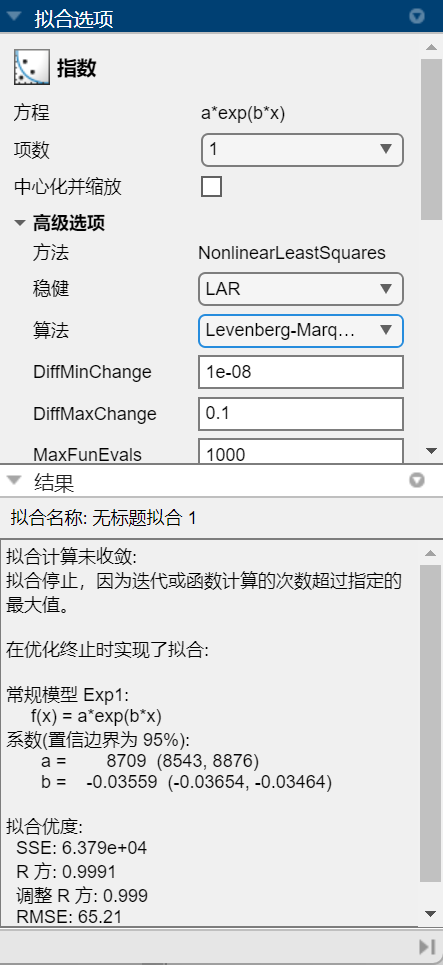
\includegraphics[width=\columnwidth]{assets/1.4/d652817bd53c95bcd5a3e9e751c357bb.png}
\caption{拟合优度}\label{1.4优度}
\end{figure}
    \end{minipage}
\end{center}

可以看到,随着外加磁场强度的增强,可逆磁导率呈以指数趋势递减,并逐渐趋于 0,符合理论预期。

\subsection{第二部分}
\subsubsection{实验一:测量模具钢的(准)静态起始磁化曲线}

实验时直接测得了 $I$ 和 $B$,只需对 $H$ 进行换算和修正:
\begin{equation}
H = \frac{N}{l_2}\cdot I = 8.3333 \times 10^3 \cdot I,\quad H_{\text{re}} = \frac{N}{l_2}\cdot I - \frac{l_g}{\mu_0 l_2}\cdot B = 8.3333 \times 10^3 \cdot I - 6.6315 \times 10^3 \cdot B
\end{equation}
\begin{figure}[H]\centering
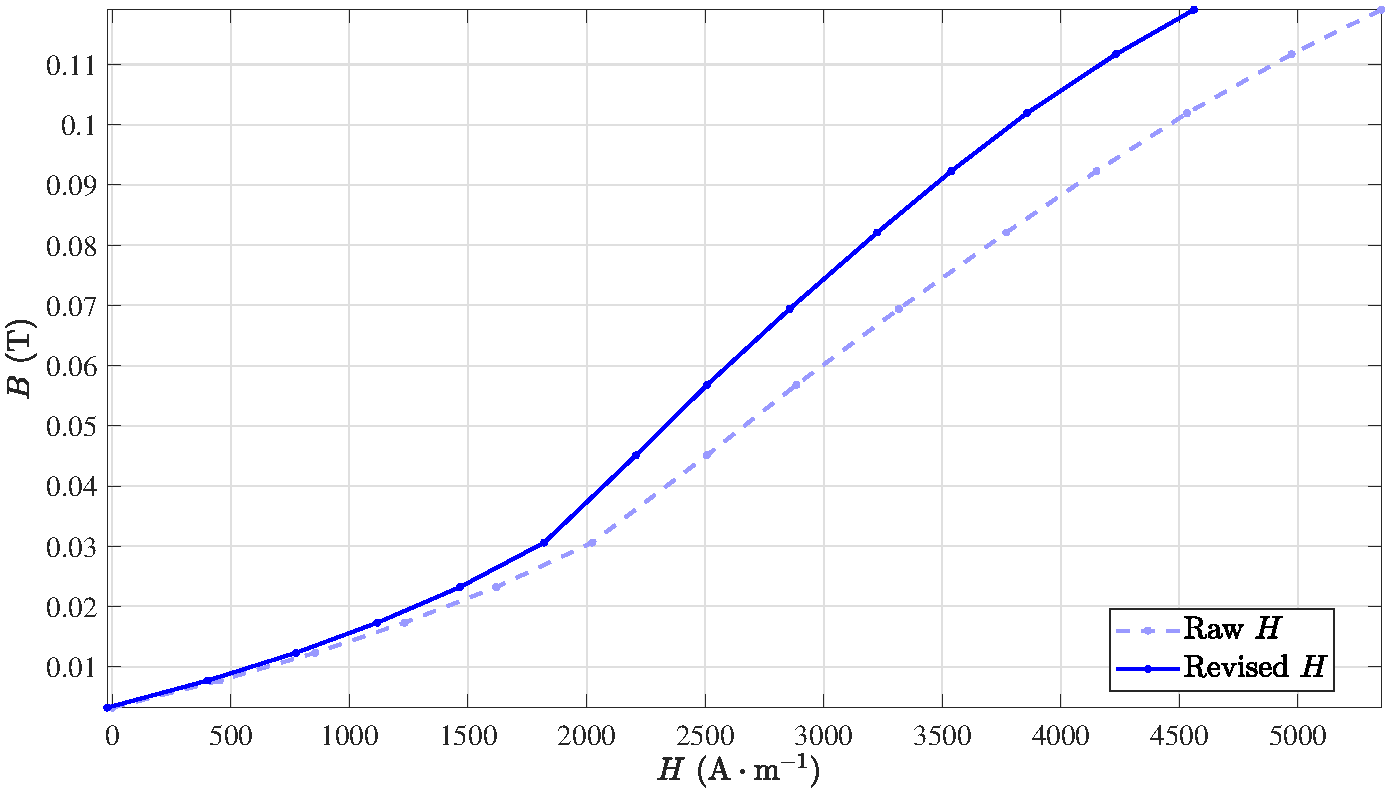
\includegraphics[width=0.85\columnwidth]{assets/2.1/2024-10-29_01-01-14.pdf}
\caption{模具钢的(准)静态起始磁化曲线}\label{2.1图}
\end{figure}

\begin{table}[H]\centering
    %\renewcommand{\arraystretch}{1.5} % 调整行间距为 1.5 倍
    %\setlength{\tabcolsep}{1.5mm} % 调整列间距
    \caption{霍尔传感器测量样品的起始磁化曲线}
    \label{2.1表}
\begin{tabular}{cccccccccc}\toprule
    $I$ (mA) & $B$ (mT) & $H \ \mathrm{(A\cdot m^{-1})}$ &  $H_{\text{re}} \ \mathrm{(A\cdot m^{-1})}$   \\
    \midrule
    0	    & 3.2	& 0.000	    & -21.221   \\
    54.4	& 7.7	& 453.333	& 402.271   \\
    102.7	& 12.3	& 855.833	& 774.266   \\
    147.9	& 17.3	& 1232.500	& 1117.776  \\
    194.3	& 23.2	& 1619.167	& 1465.317  \\
    242.9	& 30.6	& 2024.167	& 1821.244  \\
    300.9	& 45.1	& 2507.500	& 2208.421  \\
    346.2	& 56.8	& 2885.000	& 2508.333  \\
    398.0	& 69.4	& 3316.667	& 2856.444  \\
    452.5	& 82.1	& 3770.833	& 3226.391  \\
    498.1	& 92.3	& 4150.833	& 3538.750  \\
    543.9	& 101.9	& 4532.500	& 3856.755  \\
    596.8	& 111.7	& 4973.333	& 4232.600  \\
    642.2	& 119.1	& 5351.667	& 4561.860  \\
    \bottomrule
\end{tabular}
\end{table}

此小节实验较为成功,成功拟合出了大致的磁化曲线。但是,需要关注的是,受设备限制,即便采样到电流峰值 642.2 mA,磁感应强度也未达到平稳区,没有达到饱和磁化状态。

\subsubsection{实验二:测量模具钢的(准)静态磁滞回线}

计算和修正 $H$ 的方法同上一小节,这里直接给出图像和数据表。

\begin{figure}[H]\centering
\begin{subfigure}[b]{0.5\columnwidth}\centering
    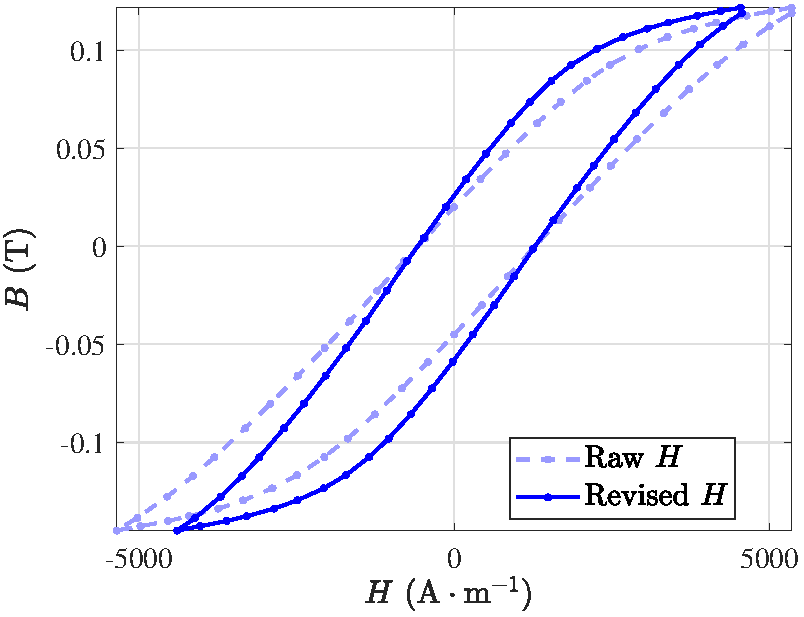
\includegraphics[height=185pt]{assets/2.2/2024-10-29_01-43-42.pdf}
    \caption{修正前后的磁滞回线对比}
\end{subfigure}\hfill
\begin{subfigure}[b]{0.5\columnwidth}\centering
    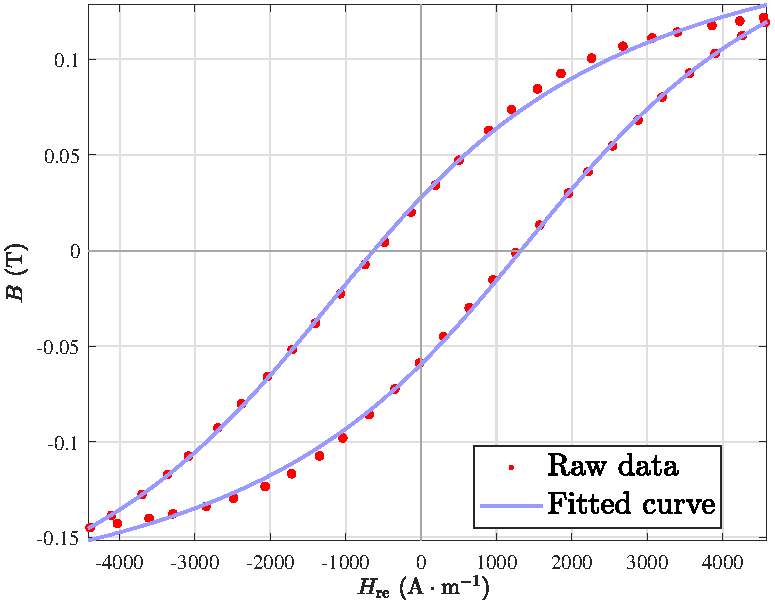
\includegraphics[height=185pt]{assets/2.2/2024-10-29_01-43-46.pdf}
    \caption{修正后的磁滞回线模型}
\end{subfigure}
\caption{模具钢的(准)静态磁滞回线}
\end{figure}

由图可以知道,修正前后的回线图像差异较大。这也启发我们,在做实验或者处理数据的过程中,不能想当然地忽略一些因素,应该就实验具体形式和数据来源等予以全面地考虑。否则得到的结果可能严重偏离实际。

\begin{table}[H]\centering
    %\renewcommand{\arraystretch}{1.5} % 调整行间距为 1.5 倍
    %\setlength{\tabcolsep}{1.5mm} % 调整列间距
    \caption{霍尔传感器测量样品的静态磁滞回线}
    \label{2.2表}
\resizebox{\linewidth}{!}{   % 设置宽度为 \linewidth 等比例缩放
\begin{tabular}{|c|cccc|c|cccc|}\hline
    序号 & $I$ (mA) & $B$ (mT) & $H \ \mathrm{(A\cdot m^{-1})}$ &  $H_{\text{re}} \ \mathrm{(A\cdot m^{-1})}$ & 序号 & $I$ (mA) & $B$ (mT) & $H \ \mathrm{(A\cdot m^{-1})}$ &  $H_{\text{re}} \ \mathrm{(A\cdot m^{-1})}$    \\
    \hline
    1	&642.2	&121.8	&5351.667	&4543.955	&28	&-597.1	&-142.7	&-4975.833	&-4029.525 \\
    2	&602.7	&120.0	&5022.500	&4226.725	&29	&-544.3	&-140.0	&-4535.833	&-3607.429 \\
    3	&556.6	&117.7	&4638.333	&3857.811	&30	&-504.4	&-137.6	&-4203.333	&-3290.845 \\
    4	&498.6	&114.2	&4155.000	&3397.688	&31	&-448.7	&-133.7	&-3739.167	&-2852.541 \\
    5	&456.0	&111.1	&3800.000	&3063.245	&32	&-401.7	&-129.5	&-3347.500	&-2488.726 \\
    6	&406.2	&106.8	&3385.000	&2676.761	&33	&-346.6	&-123.4	&-2888.333	&-2070.012 \\
    7	&351.5	&100.6	&2929.167	&2262.042	&34	&-299.0	&-116.7	&-2491.667	&-1717.776 \\
    8	&296.2	&92.5	&2468.333	&1854.924	&35	&-247.0	&-107.4	&-2058.333	&-1346.115 \\
    9	&252.5	&84.5	&2104.167	&1543.809	&36	&-202.7	&-98.0	&-1689.167	&-1039.284 \\
    10	&202.7	&73.7	&1689.167	&1200.428	&37	&-151.1	&-85.7	&-1259.167	&-690.851  \\
    11	&157.8	&62.8	&1315.000	&898.545	&38	&-99.5	&-72.4	&-829.167	&-349.049  \\
    12	&97.7	&47.2	&814.167	&501.162	&39	&-49.7	&-58.9	&-414.167	&-23.574   \\
    13	&50.1	&34.2	&417.500	&190.704	&40	&0.0	&-44.9	&0.000	    &297.752   \\
    14	&0.0	&20.1	&0.000	    &-133.292	&41	&52.7	&-29.9	&439.167	&637.447   \\
    15	&-54.5	&4.3	&-454.167	&-482.682	&42	&102.3	&-15.3	&852.500	&953.961   \\
    16	&-95.1	&-7.3	&-792.500	&-744.090	&43	&149.5	&-1.2	&1245.833	&1253.791  \\
    17	&-146.4	&-22.6	&-1220.000	&-1070.129	&44	&199.5	&13.3	&1662.500	&1574.302  \\
    18	&-198.4	&-38.0	&-1653.333	&-1401.338	&45	&258.3	&30.0	&2152.500	&1953.556  \\
    19	&-246.5	&-51.8	&-2054.167	&-1710.657	&46	&298.5	&41.2	&2487.500	&2214.284  \\
    20	&-297.2	&-65.9	&-2476.667	&-2039.654	&47	&348.1	&54.7	&2900.833	&2538.093  \\
    21	&-349.7	&-80.2	&-2914.167	&-2382.324	&48	&399.6	&68.2	&3330.000	&2877.735  \\
    22	&-397.3	&-92.7	&-3310.833	&-2696.097	&49	&447.3	&80.2	&3727.500	&3195.657  \\
    23	&-456.2	&-107.5	&-3801.667	&-3088.785	&50	&501.0	&92.7	&4175.000	&3560.264  \\
    24	&-497.1	&-117.1	&-4142.500	&-3365.957	&51	&550.1	&103.0	&4584.167	&3901.127  \\
    25	&-545.9	&-127.6	&-4549.167	&-3702.993	&52	&600.4	&112.3	&5003.333	&4258.621  \\
    26	&-602.8	&-138.4	&-5023.333	&-4105.540	&53	&642.4	&119.1	&5353.333	&4563.527  \\
    27	&-642.3	&-144.9	&-5352.500	&-4391.602	&	&		&	& & \\
    \hline
\end{tabular}}
\end{table}

\section{思考题}

\subsection*{6.1 铁磁材料的动态磁滞回线与(准)静态磁滞回线在概念上有什么区别?铁磁材料动态磁滞回线的形状和面积受那些因素影响?}


\noindent \textbf{(1) 区别:}

动态磁滞回线是指铁磁材料在交变磁场作用下得到的一条闭合$ B-H $曲线。而静态磁滞回线是指铁磁材料在恒稳磁场下完全磁化后的$ B-H $曲线,实际测量时会选择在磁场强度$ H $的一个周期内缓慢改变其值,测定此时的$ B $,进而得到(准)静态磁滞回线。

对于静态磁滞回线而言,一次循环磁化过程中的能量损耗(这于$ B-H $曲线所包围的面积成正比)仅包括磁滞损耗;而对于动态磁滞回线,一次循环磁化过程中的能量损耗除了磁滞损耗,还包括涡流损耗、剩余损耗等,这些损耗也受多种因素影响。

\noindent \textbf{(2) 影响因素:}

铁磁材料动态磁滞回线的形状和面积受材料本身性质、外磁场的频率与幅度等多方面影响。

材料本身的矫顽力越小,磁滞回线的形状越窄;一般地,对属于金属氧化物的铁氧体而言,其电阻率较高,所以交变外磁场的频率越大、幅度越小时,磁滞回线所包围的面积越小,磁滞损耗越小;而对硅钢体来说,外磁场的频率越大、磁滞回线包围面积也越大,磁滞损耗越大;

另外,相同条件下,材料的电阻率越低,涡流损耗会越大。


\subsection*{6.2 什么叫做基本磁化曲线?它和起始磁化曲线间有何区别?}

\noindent\textbf{(1) 初始磁化曲线:}

磁性材料的磁化和磁化历史有关系,对一个未磁化过(或经过充分消磁)的磁性材料,从 0 开始缓慢增大 $H$ 值,$B$ 值也随着增大。但当 $H$ 值增大到足够大时,$B$ 值就不再增加,材料达到饱和磁化,此时 $B = B_s$。这个过程的 $H$-$B$ 曲线就是。

\noindent\textbf{(2) 基本磁化曲线:}

用不同的交变外磁场幅度 $H_m$ 对材料进行磁化,可以得到一系列磁滞回
线,把这些磁滞回线的顶点连线所得的线,就称作。

\noindent\textbf{(3) 区别:}

基本磁化曲线是不同的静态磁滞回线的顶点相连形成的曲线,而起始磁化曲线是一族(多条)动态磁滞回线的顶点相连形成的曲线。前者是静态的,而后者是动态的。

简单来讲,初始磁化曲线是“恒定”外磁场下的得到的曲线,而基本磁化曲线是“交变”外磁场下得到的曲线。两种曲线是用不同的实验方法得到的不同曲线,但它们在某些区域是近似相等的。


\subsection*{6.3 铁氧体和硅钢材料的动态磁化特性各有什么特点?}

\noindent\textbf{(1) 磁化特性:}

铁氧体材料比硅钢材料更容易磁化且其磁导率更高,矫顽力更小,因此磁滞损耗也更小。同时,铁氧体单位体积中存储的磁能更低,饱和磁化强度也更低。相反,硅钢材料磁导率低,磁化难,矫顽力大,需要更大的磁场才能让材料的磁性逆转。

\noindent\textbf{(2) 磁滞损耗:}

随频率的增大,二者的磁滞耗损变化也不同。铁氧体磁滞耗损逐渐变小,而硅钢的耗损增大。也因此,硅钢片通常用于低频变压器而铁氧体通常用于高频变压器。这些结论可以从第 \ref{铁氧体} (2) 节和第 \ref{不同频率硅钢} 节的实验中得到。

\subsection*{6.4 动态磁滞回线测量实验中,电路参量应怎样设置才能保证$u_{R_1}-u_C$所形成的李萨如图形正确反映材料动态磁滞回线的形状?}

一方面,外磁场的周期 $T$ 应该远小于积分常量,即 $T \ll R_2C$,
这是因为推导公式 $B=\frac{R_2 C}{N_2 S}u_c$ 时,需要用到积分近似 $u_c=\frac{1}{R_2 C}\int u_2\mathrm d t$,这里就要求$T \ll R_2C$。另一方面,交流激励的幅度应当充分大,以便使铁磁体能够充分磁化。

如果达不到上面的要求,测得的磁滞回线可能变形,与真实的动态磁滞回线有较大差别,从第 \ref{铁氧体} (3) 节的实验中可以看到这一点。

\subsection*{6.5 准静态磁滞回线测量实验中,为什么要对样品进行磁锻炼才能获得稳定的饱和磁滞回线?}

受磁化历史影响,对同一外磁场 $H_m$,材料可能具有不同的剩磁,所以对应的 $B_m$ 值也不同。这是就需要进行充分的磁锻炼。磁锻炼,即反复进行正反向饱和磁化,消除磁介质中剩有的磁阻力,此时进行实验才能得到一个中心对称的静态磁滞回线。


\section{实验总结与心得体会}

此次实验总共分为两部分,第一部分是利用磁特性综合测量实验仪,将磁感应强度、磁场强度等磁学量转化为电压信号进行测量,用示波器进行可视化;
第二部分是利用霍尔传感器测量并绘制样品材料的静态磁滞回线。两部分内容相互呼应,既丰富了实验的内容,又增加了趣味性。

实验总体上是成功的,几乎所有小节的实验都与理论符合得很好,实验数据和图像也十分具有说服力。

特别地,本次实验我利用了 Matlab 软件对实验数据作进一步的处理和分析,包括换算、拟合、可视化等,相比于常规数据处理和画图方法,这大大提高了分析的准确性和图像的美观性。在今后的实验和研究工作中,我还会继续深入学习和应用类似地计算软件,增强自己的科学计算能力。科研不是考试,我们应该充分利用好自己能接触到的资源,合理使用工具,更高效地发展自身。

另外,这次实验让我感受到,实验“结束”并不意味着实验就已经完成,事实上这仅是数据测量的结束。在课后,我们还需要重新整理实验原理和过程,换算、分析、拟合实验数据,作出合适的数据图,对实验现象进行讨论,解释可能存在的误差等。在根据已有数据求所需结果时,如何才能最大程度地利用已有数据,同时又尽可能地降低二次误差。上面这些内容都需要体现在最终的实验报告中,一点点累加起来,着实花费了我很多精力。

但最后回过头来再看,我认为一切都是值得的。当处理完毕的结果十分有力地验证了理论值时,当作出的数据图像近乎“完美”地与理论契合时,心中便迸发出无尽的喜悦,也深深感受到物理“理论与实验结合”的魅力。\footnote{手写预习报告、原始数据记录表和 Matlab 源代码附在附录中。}




% --------------------------- 附录 --------------------------- %
% >> ------------------------ 附录 ------------------------ << %


\newpage
\appendix
% section 标题自定义设置 
\titleformat{\section}[hang]{\normalfont\huge\bfseries\centering}{}{20pt}{}
\titlespacing*{\section}{0pt}{-25pt}{8pt} % 控制上方空白的大小
% subsection 标题自定义设置 
\titleformat{\subsection}[hang]{\normalfont\Large\bfseries\boldmath}{\thesubsection}{8pt}{}
% subsubsection 标题自定义设置 
\titleformat{\subsection}[hang]{\normalfont\normalsize\bfseries\boldmath}{\thesubsection}{8pt}{}


% 附录 A
\section*{附录 A\hspace*{20pt} 手写预习报告}
\addcontentsline{toc}{section}{附录 A\hspace*{6pt} 手写预习报告} 
\thispagestyle{fancy} 

\begin{figure}[H]\centering
    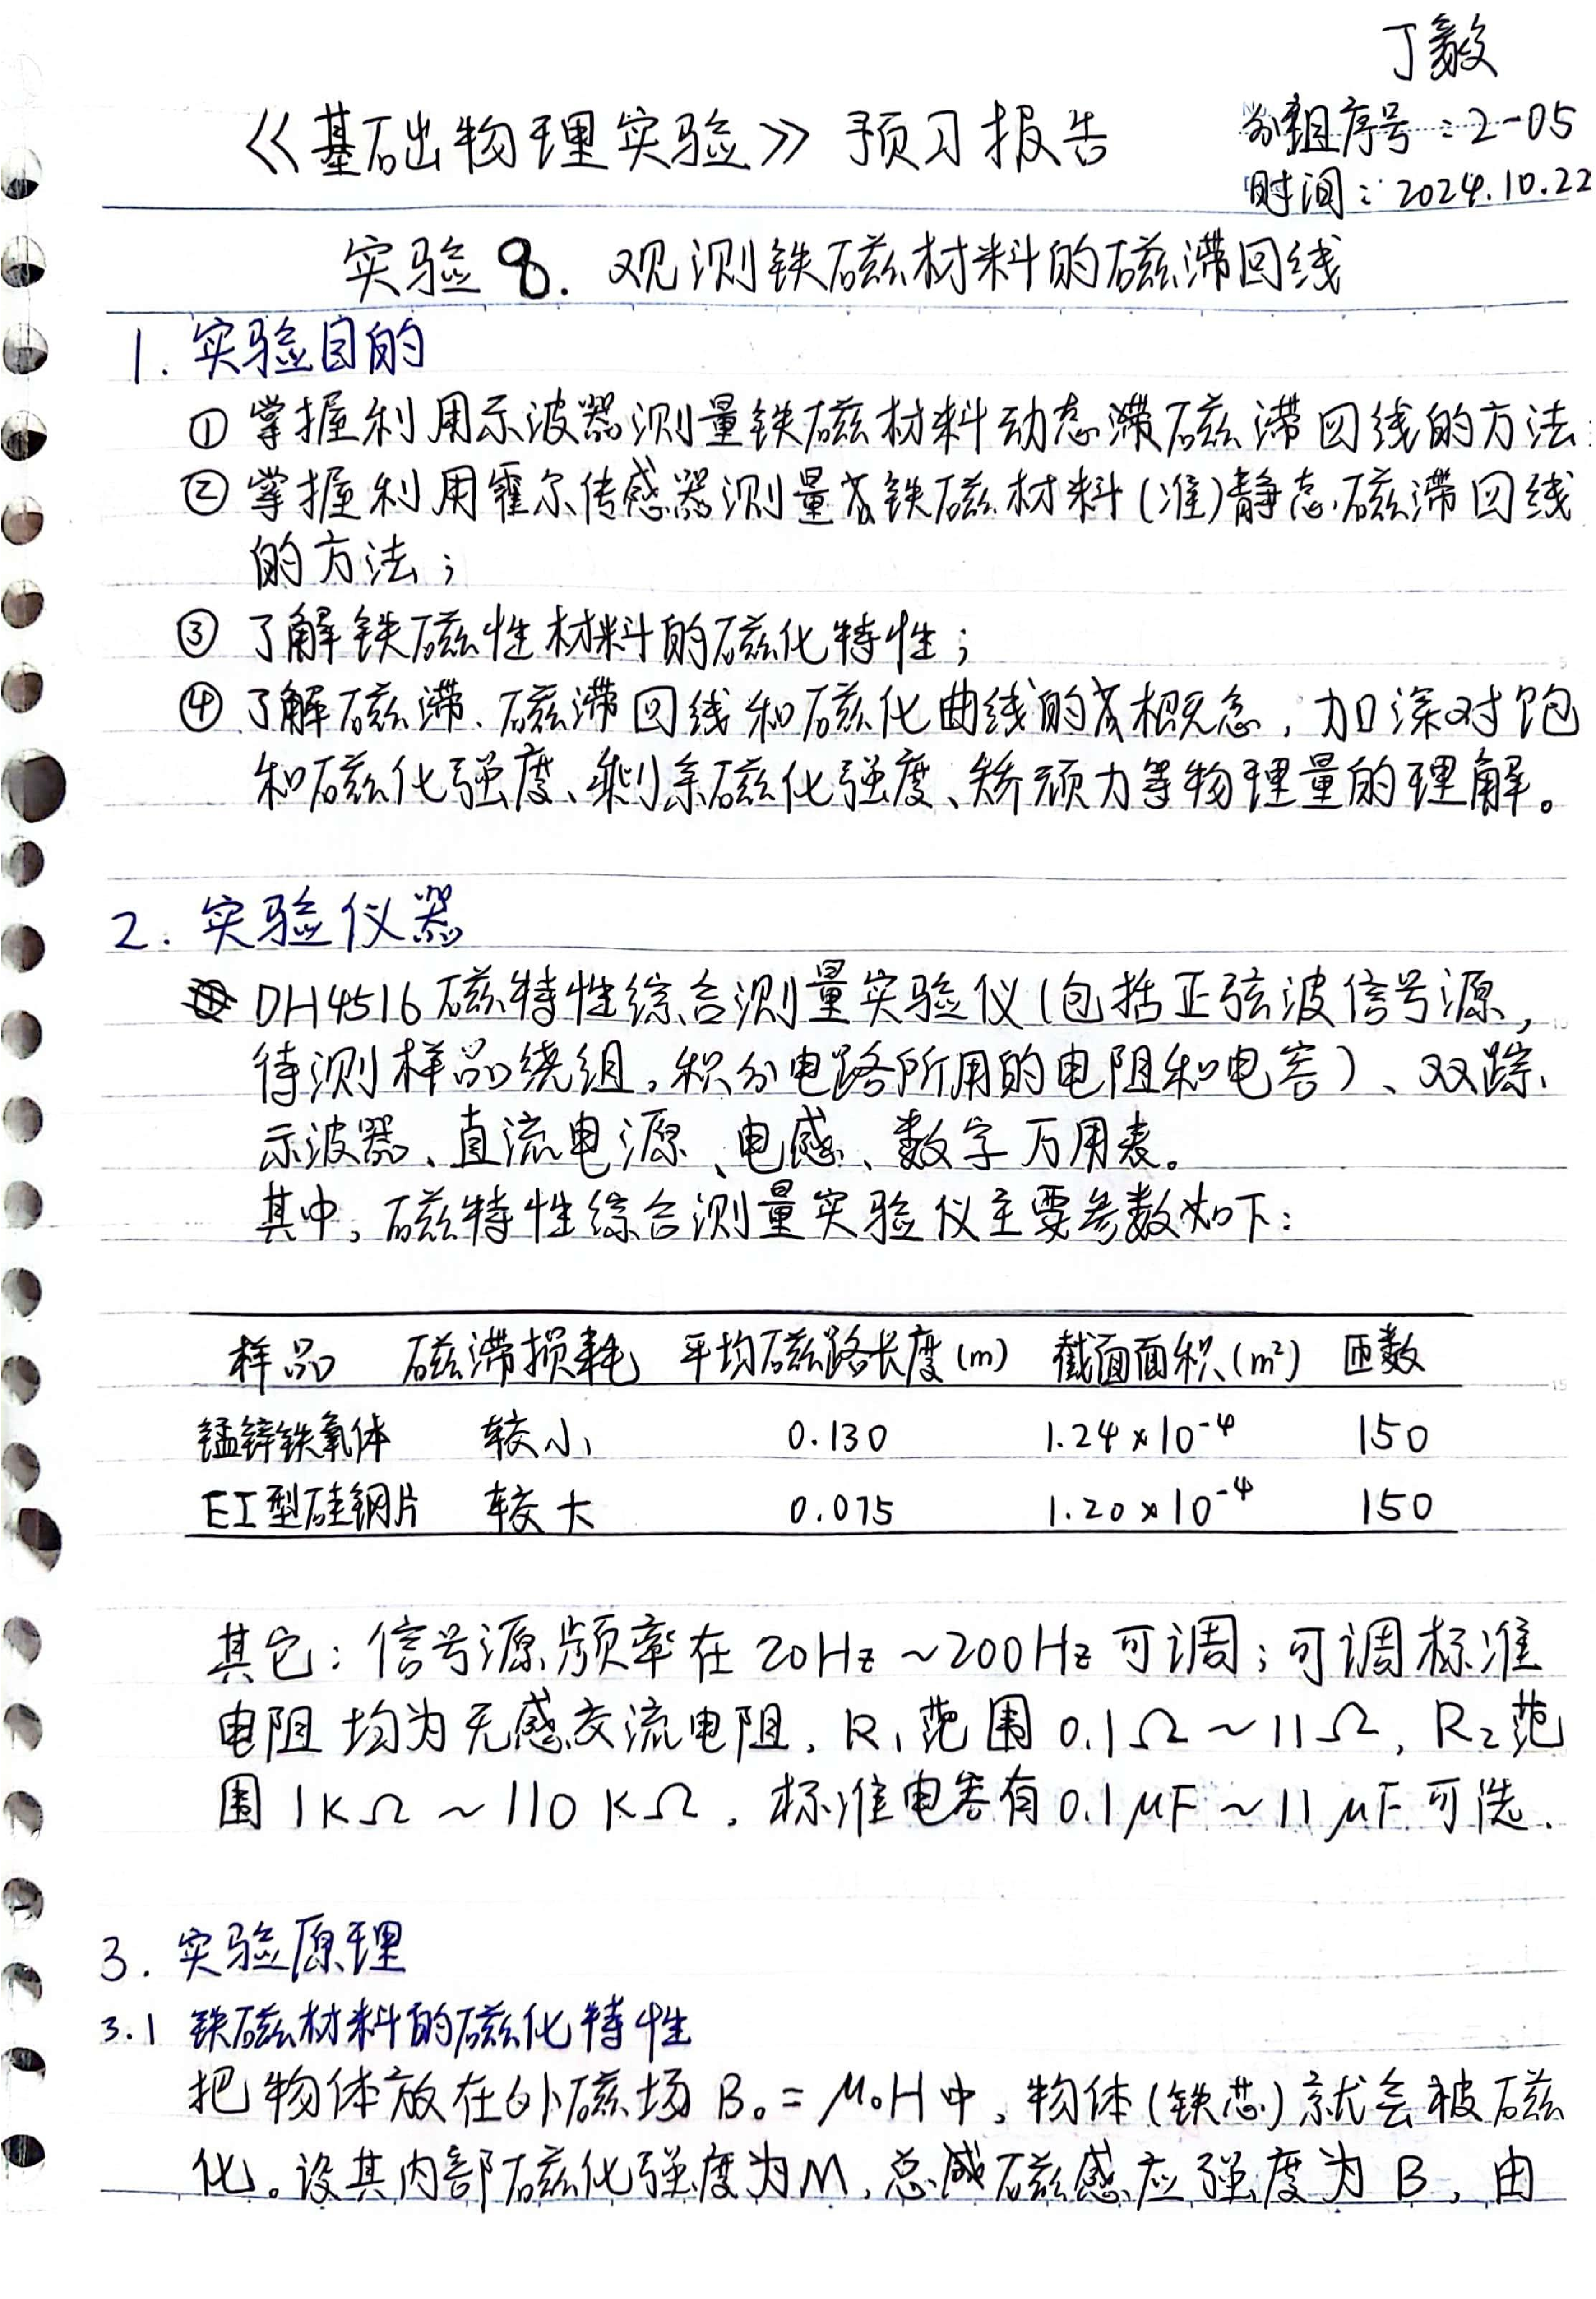
\includepdf[pages=1, width=500pt]{pdf/预习报告-2-05组-丁毅-磁滞回线-2024.10.22-朱中柱.pdf}
\end{figure}
\includepdf[pages={2}]{pdf/预习报告-2-05组-丁毅-磁滞回线-2024.10.22-朱中柱.pdf}


% 附录 B
\section*{附录 B\hspace*{20pt} 原始数据记录表}
\addcontentsline{toc}{section}{附录 B\hspace*{6pt} 原始数据记录表} 
\thispagestyle{fancy} 

\begin{figure}[H]\centering
    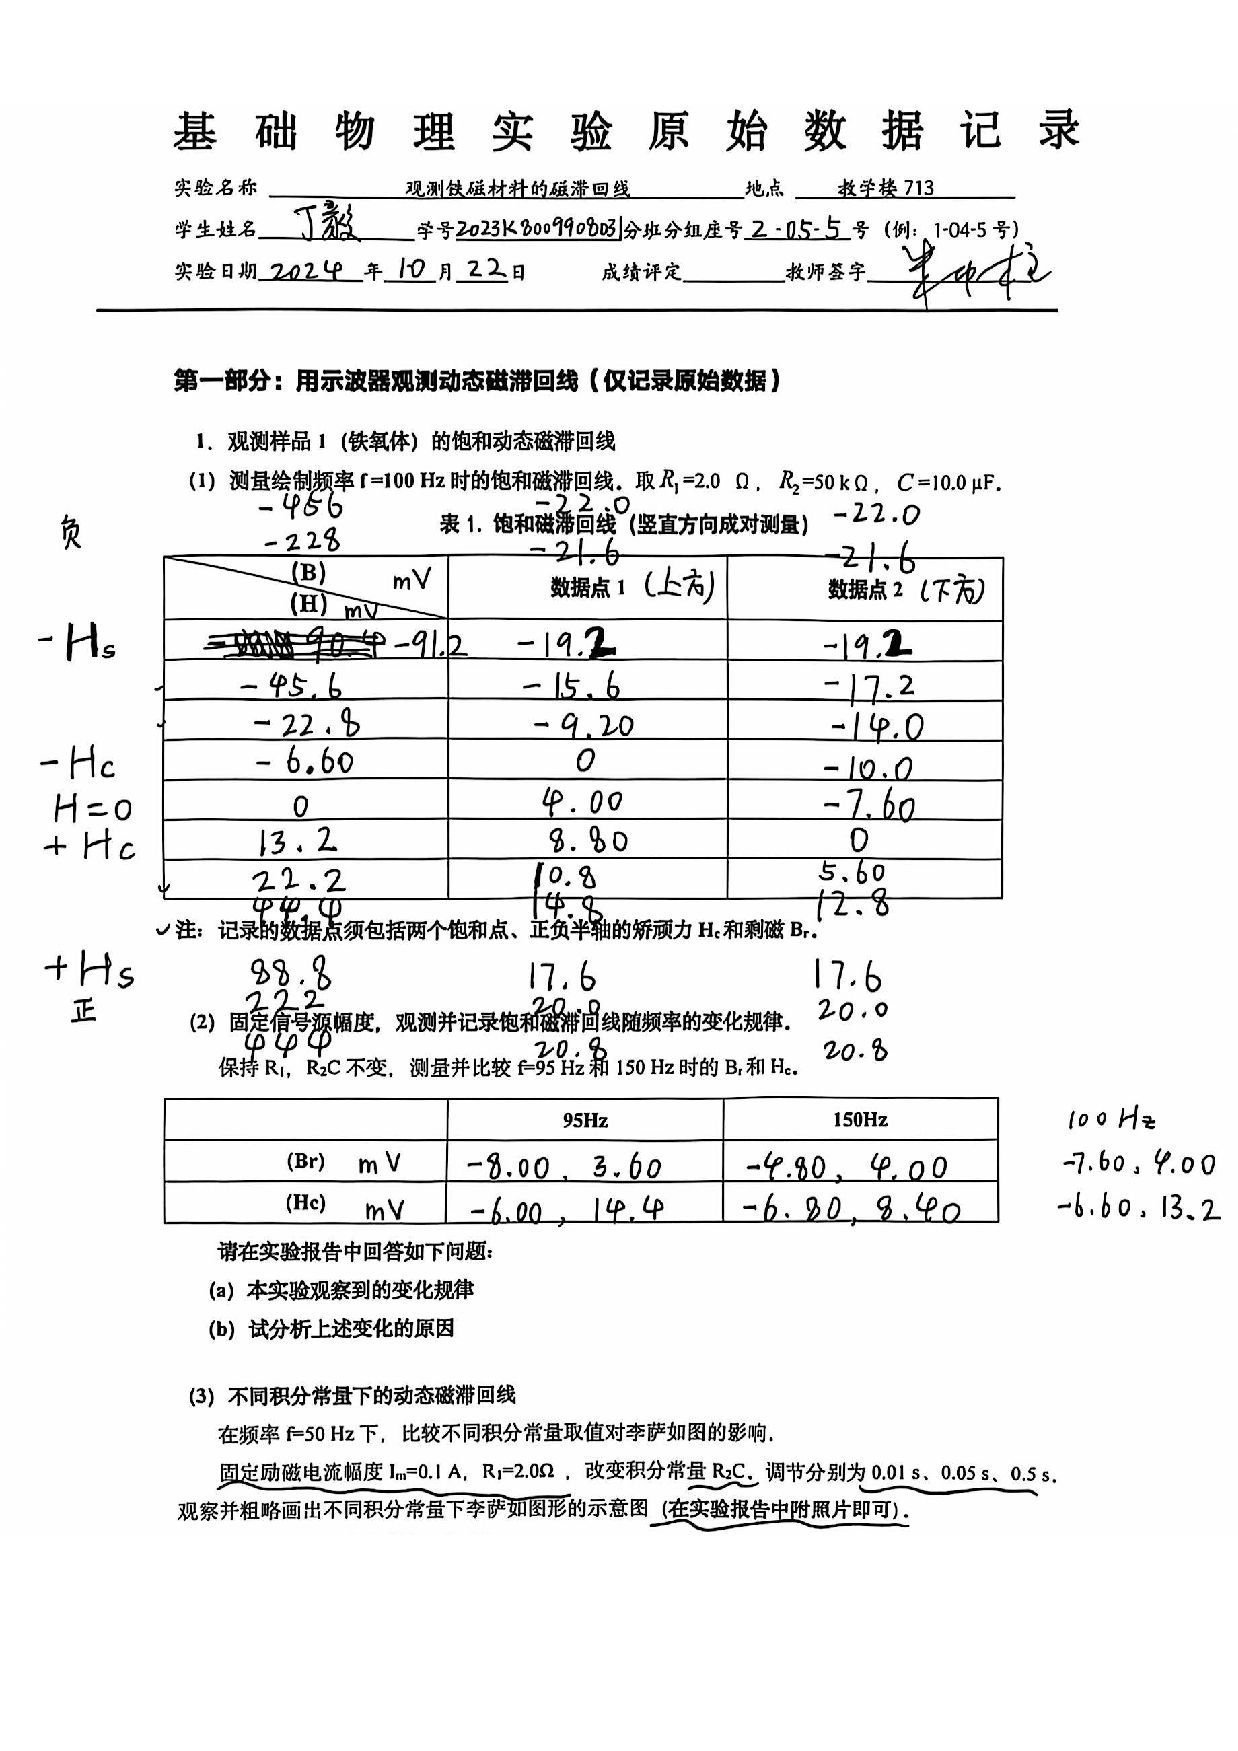
\includepdf[pages=1, width=500pt]{pdf/原始数据-2-05组-丁毅-磁滞回线-2024.10.22-朱中柱.pdf}
\end{figure}
\includepdf[pages={2-4}]{pdf/原始数据-2-05组-丁毅-磁滞回线-2024.10.22-朱中柱.pdf}


% 附录 C
\section*{附录 C\hspace*{20pt} Matlab 源码}
\addcontentsline{toc}{section}{附录 C\hspace*{6pt} Matlab 源码} 
\thispagestyle{fancy} 

% 目录不够放了,只能出此下策
{\normalfont\Large\bfseries\boldmath 
\begin{center}
    C.1 第一部分
\end{center}
}

{\noindent\normalfont\large\bfseries\boldmath C.1.1 实验一图 \ref{1.1图} 源码}\label{1.1源码}
\lstinputlisting{d:/a_RemoteRepo/GH.MatlabCodes/本科课程代码/基础物理实验/Ex_8/Ex_8_Part1_1.m}

{\noindent\normalfont\large\bfseries\boldmath C.1.2 实验二图 \ref{1.2图} 源码}\label{1.2源码}
\lstinputlisting{d:/a_RemoteRepo/GH.MatlabCodes/本科课程代码/基础物理实验/Ex_8/Ex_8_Part1_2.m}

{\noindent\normalfont\large\bfseries\boldmath C.1.3 实验四图 \ref{1.4图} 源码}\label{1.4源码}
\lstinputlisting{d:/a_RemoteRepo/GH.MatlabCodes/本科课程代码/基础物理实验/Ex_8/Ex_8_Part1_4.m}

\end{document}

% VScode 常用快捷键:

% F2:                       变量重命名
% Ctrl + Enter:             行中换行
% Alt + up/down:            上下移行
% 鼠标中键 + 移动:           快速多光标
% Shift + Alt + up/down:    上下复制
% Ctrl + left/right:        左右跳单词
% Ctrl + Backspace/Delete:  左右删单词    
% Shift + Delete:           删除此行
% Ctrl + J:                 打开 VScode 下栏(输出栏)
% Ctrl + B:                 打开 VScode 左栏(目录栏)
% Ctrl + `:                 打开 VScode 终端栏
% Ctrl + 0:                 定位文件
% Ctrl + Tab:               切换已打开的文件(切标签)
% Ctrl + Shift + P:         打开全局命令(设置)

% Latex 常用快捷键:

% Ctrl + Alt + J:           由代码定位到PDF


